% ============================================================
%  第七章 氧化物高温超导体和各向异性超导电性（§1–§8 + 章末参考文献）
%  底本：高等教育出版社《固体理论》第二版；原书印刷页 229–285
%  （PDF 页 = 印刷页 + 20）
%  公式编号自检：§3 (7.3.1)–(7.3.4)；§4 (7.4.1)–(7.4.45)
%    （(7.4.13a/b)、(7.4.23a/b)、(7.4.30a/b)、(7.4.32a/b)、
%    (7.4.33a/b)、(7.4.34a/b) 为原书自带二级编号，用 subequations
%    环境照录，与 ch04/ch06 体例一致）；§5 (7.5.1)–(7.5.7)；
%    §6 (7.6.1)–(7.6.19)；§7 (7.7.1)–(7.7.14)。
%    全章自动编号 89 个，各节均无缺号。
%
%  任务单所列 6 处"缺号"逐条对照原书页面判定（均非原书跳号）：
%    (7.4.1)  原书 p252 在号（OCR 乱码）；
%    (7.5.2)  原书 p261 在号（OCR tag 误作逗号 7.5,2）；
%    (7.5.4)  原书 p261 在号（OCR tag 本在）；
%    (7.5.6)  原书 p263 在号（OCR tag 残缺作 (.6)，已按页面补排）；
%    (7.6.9)  原书 p267 在号（OCR 乱码，已按页面补排）；
%    (7.7.12) 原书 p276 在号（OCR tag 断作 (7.7.+12）。
%  另：OCR 中 \tag{C.7} 为所引附录 C 公式编号（原书 p256 照排
%    (C.7)），用 \tag 照录，不占章内公式计数。
%
%  已修正的 OCR/原书错误（除全角句点转"."、删 ~ 间隔符、收紧
%  \mathrm{d}、拆开行内公式与中文等常规项外）：
%  1. 表 7.1 OCR 串行，按 p230 原表逐格复原（Hg-1223 之 H_c
%     值原书即空缺）；O_{10+1}→O_{10+x}。
%  2. §1 HoMo_6S_6（OCR 误作 H_0M_06S_6、ΔT_c=2ΔK）按 p230 复原；
%     "在加高压条件下 T_c 一般仍限于 10 K 之内"语序按 p230 复原；
%     "载流子流度"→"载流子浓度"、"确实出人意料"等粘连按 p231 复原；
%     La-Ba-Cu-O、La_2-xM_xCuO_4、Nd_2-xCe_xCuO_4 等化学式按
%     p231–232 复原；"superrcon-ducting"→superconducting。
%  3. §1 "交换反铁磁自旋涨落"原书漏"磁"字（p230），按文意补。
%  4. §2 "这些结构均具有正交对称性"OCR"匀"→均（p235）；"例如在
%     La-214 与 Bi-2201 中"OCR 串行按 p235 复原；"引人"→引入
%     （p238）；图 7.2(b) YBa_2Cu_3O_{6+x}（OCR Cu_8）；"超导相干
%     长度"OCR"相于"→相干（p245）。
%  5. §2.1 (ii) 结构单元图示与 (iii) La-214 掺杂表格 OCR 乱码，
%     按 p236–237 原书复原（La^{3+}_{1-x/2}(Sr^{2+})_{x/2}O^{2-}_4
%     等按原书照排）。
%  6. (7.3.1) arctan(k_y/k_x) OCR 多余 \mid 已删（p243 无绝对值）。
%  7. §3.1 "两个载流配对"原书如此（p241），照录。
%  8. §3.2 "扫描述磁强计""半整的量子磁通""首先制了成全由"等
%     原书排印如此（p244），照录。
%  9. 表 7.2 按 p245 原表复原；Nb 行 λ、ξ 为合并格。
% 10. (7.4.10) 第二等式积分下标 FS（OCR 误作 F^3，p253）；
%     (7.4.12) 第二行 Y_{l'm'} 补撇；(7.4.13b) 积分内 ψ_l(k') 与
%     积分限 ε_{k'} 按 p253 复原（OCR 误作 φ、ε_k）。
% 11. (7.4.15) 按 p253 复原：∫_0^{ħω_0} dε/(2ε-E)（OCR 乱码）。
% 12. (7.4.23b) 等号后原书衍一竖线"|"（p256 排印残迹），已删。
% 13. (7.4.26) OCR 之 \hat\theta、\hat\delta 按 p256 复原为 δ；
%     末尾逗号已删。
% 14. 表 7.5 按 p254 复原（单重态自旋波函数 (↑↓-↓↑)/√2）。
% 15. (7.4.34a)、(7.4.39)、(7.4.42) OCR 严重乱码按 p258、260 复原。
% 16. §5 (7.5.3)(7.5.4)(7.5.5) 按 p261 复原（Σ 积分域、cases）；
%     (7.5.6) 中间情形 (1/i)∫_{-1}^{1}dx/√(x^2-(ω/Δ_0)^2) 按 p263
%     复原；(7.5.7) cases 按 p263 复原。
% 17. §5.2 "重费密子超导体具有奇异特性"OCR 漏"子"（p264）；
%     "表中的低温比热容……"固体物理公式按 p264 复原。
% 18. 表 7.6 按 p264 原表逐格复原（c_es 行 ~T^{2.8}、~T^{2.86} 等；
%     T_{1s}^{-1} 行 ~T^3(^{63}Cu)、~T^3(^{9}Be)、~T^3(^{195}Pt)；
%     Δλ 行 d 波极向态 {T(纯); T^2(含杂)}）。
% 19. §5.2"仔细分析表7.5中"与 §6.2"表7.5中所用的固体物理学公式"
%     两处原书引号有误：所指均为表 7.6 及其下注公式，按 p264/266
%     更正为表 7.6。
% 20. (7.6.2) 按 p265 复原（OCR 乱码）；(7.6.9) 按 p267 复原；
%     §6.3 二维能隙方程（未编号）及零温能隙推导诸式（未编号）
%     按 p268 复原；(7.6.14) OCR \bigcup(0)→Δ_0(0)、Ψ_d→V_d。
% 21. (7.7.13) OCR 乱码按 p277 复原；"约飞(Ioffe)判据"按 p272
%     复原；图 7.14 图注原书"核自系统"漏"旋"字（p277），补为
%     "核自旋系统"。
% 22. §7.1 ρ_0 句"ρ_0 为将 ρ_ab(T) 的线性关系外延到绝对零度时的
%     插值"按 p271 复原。
% 23. §8.2 "研究组[35]"补全上标括号；Δ_BCS(T_c)=0 按 p283 复原；
%     (7.6.1) 中 φ=arctan(k_y/k_x)（OCR 衍符已清）。
% 24. §3.4 "但在解释同位素效应时却是不可忽略的"OCR 漏"可"
%     （p250），按原书补。
%  遗留问题：
%  · 图 7.1–7.17 均为占位图（figures/fig7-N.pdf），重绘代理负责；
%    图 7.2、7.6、7.7、7.16 原书为多图（(a)/(b) 或 (a)/(b)/(c)）
%    结构，图注按原书补子图说明。
%  · 原书 p244 "扫描述磁强计""半整的量子磁通"、p244 "首先制了成"
%    、p241 "两个载流配对"、p250 "弱杂的Y-123"、p281 "使态k态的
%    态密度"等均系原书排印如此，未改动。
%  · 原书用字"费密"照录；仅 p239 一处"费米液体"原书即作"费米"，
%    照录未改。
% ============================================================
\chapter{氧化物高温超导体和各向异性超导电性}

本章主要介绍铜氧化合物高温超导体的基本属性.我们将首先对提高超导转变温度的历史进程作一个简单的回顾（§1），然后介绍高温超导体的结构与相图（§2）以及超导态（§3）的共同特征.为了理解高温超导体的超导态与BCS超导态的不同之处，我们将先介绍各向异性配对的超导理论（§4、§5），然后用此理论来解释高温超导体的异常超导特性（§6）.最后，介绍高温超导体正常态的反常特性（§7）以及在弱掺杂区发现正常态能隙所提出的物理问题（§8）.

\section{\texorpdfstring{高$T_{\mathrm{c}}$——超导电性研究的重大突破}{高Tc——超导电性研究的重大突破}}

自从1911年昂内斯（Kammerlingh Onnes）在4.2 K发现 $\mathrm{Hg}$ 的超导电性以来，提高超导转变温度 $T_{\mathrm{c}}$ 就已经成为超导电性研究的主要目标之一，经过许多科学家的长期探索，人们已发现了千余种常规超导体，包括元素超导体及合金与化合物超导体.在元素周期表中，已经发现具有超导电性的元素超过了50种，其中在常压室温下为典型半导体的 $\mathrm{Ge}$ 和 $\mathrm{Si}$，通过加高压（约200 kbar）使之金属化以后，也可进入超导态，并测得 $T_{\mathrm{c}}=6.7$ K（Si）和5.3 K（Ge），其它的在高压下才发现具有超导电性的元素还有P、As、Se、Y、Sb、Te、Cs、Ba、Bi、Ce和U等.尽管如此，在元素超导体中测得的最高转变温度是 $T_{\mathrm{c}}=9.3$ K（Nb），仍处于液He温区，而且元素超导体的临界磁场 $H_{\mathrm{c}}$ 一般都很低，无应用价值，如表7.1所示\textsuperscript{[1]}.

为了获得具有实用价值的超导材料，从20世纪60年代起人们又发现配制超导合金与化合物可进一步提高 $T_{\mathrm{c}}$ 和 $H_{\mathrm{c}}$，并成功地用 Nb-Ti 合金制成了可在4.2 K工作的10 T的超导磁体.只是数十年来 $T_{\mathrm{c}}$ 的提高十分缓慢，直至1973年才在 $\mathrm{Nb}_{3}\mathrm{Ge}$ 超导薄膜中观测到 $T_{\mathrm{c}}=27.3$ K，使超导进入液氢温区，对应用并未带来方便.因此，寻找更高转变温度的超导体仍是科学家梦寐以求的目标.

表7.1\quad 超导转变温度和临界磁场提高的编年表

\begin{center}\small
\begin{tabular}{clccc}
\hline
 & 超导体 & $T_{\mathrm{c}}$/K & $H_{\mathrm{c}}$/T & 观测年代\\
\hline
常规超导体 & $\mathrm{Hg}$ & 4.2 & 0.04 & 1911\\
 & $\mathrm{Pb}$ & 7.2 & 0.08 & 1913\\
 & $\mathrm{Nb}$ & 9.3 & 0.20 & 1930\\
 & Nb-Ti合金 & 10.0 & 14 & 1954\\
 & $\mathrm{V}_{3}\mathrm{Si}$ & 17.1 & 21 & 1954\\
 & $\mathrm{Nb}_{3}\mathrm{Sn}$ & 18.1 & 24 & 1954\\
 & $\mathrm{Nb}_{3}\mathrm{Ge}$ & 27.3 & 38 & 1973\\
\hline
高温超导体 & $\mathrm{La}_{2-x}\mathrm{Sr}_{x}\mathrm{CuO}_{4}$（La-214） & 40 & 40 & 1986\\
 & $\mathrm{YBa}_{2}\mathrm{Cu}_{3}\mathrm{O}_{6+x}$（Y-123） & 92 & $>$100 & 1987\\
 & $\mathrm{Bi}_{2}\mathrm{Sr}_{2}\mathrm{Ca}_{2}\mathrm{Cu}_{3}\mathrm{O}_{10+x}$（Bi-2223） & 110 & $>$120 & 1988\\
 & $\mathrm{Tl}_{2}\mathrm{Ba}_{2}\mathrm{Ca}_{2}\mathrm{Cu}_{3}\mathrm{O}_{10+x}$（Tl-2223） & 125 & $>$130 & 1988\\
 & $\mathrm{HgBa}_{2}\mathrm{Ca}_{2}\mathrm{Cu}_{3}\mathrm{O}_{8+x}$（Hg-1223） & 133（$>$160加压） & & 1993\\
\hline
\end{tabular}
\end{center}

为了改写常规超导体中 $T_{\mathrm{c}}=27.3$ K的最高纪录，1973年以后科学家们想方设法进行开拓.他们首先在稀土三元化合物 $\mathrm{ErRh}_{4}\mathrm{B}_{4}$（$T_{\mathrm{c}}=8.7$ K）及 $\mathrm{HoMo}_{6}\mathrm{S}_{6}$（$T_{\mathrm{c}}=2$ K）中发现了铁磁超导体，又在 $\mathrm{GdMo}_{6}\mathrm{S}_{8}$（$T_{\mathrm{c}}=1.4$ K，$T_{\mathrm{N}}=0.95$ K）与 $\mathrm{TbMo}_{6}\mathrm{S}_{8}$（$T_{\mathrm{c}}=1.65$ K，$T_{\mathrm{N}}=1$ K）等材料中发现了反铁磁超导体，并展开了磁与超导相互竞争与共存的研究.继之，又在低维（准一维与准二维）的有机化合物中发现了超导电性，这类有机超导体的载流子浓度很低，还存在着磁性与超导电性之间的相互竞争现象，是探索超导新机制的一个重要领域，但其转变温度不高，在加高压条件下 $T_{\mathrm{c}}$ 一般仍限于10 K之内.1979年以后，人们又在含稀土与锕系元素的金属间化合物中找到了新的一类超导体：$\mathrm{CeCu}_{2}\mathrm{Si}_{2}$（$T_{\mathrm{c}}=0.5$ K）、$\mathrm{UBe}_{13}$（$T_{\mathrm{c}}\approx1$ K）及 $\mathrm{UPt}_{3}$（$T_{\mathrm{c}}\approx0.54$ K），其超导电性与 Ce 及 U 中具有很高有效质量（$m^{*}\geqslant200\,m_{\mathrm{e}}$）的4f 及 5f 电子有关，故称为重费密子超导体（HFS）.重费密子超导体属于强关联电子体系（同一格点上的4f或5f电子间存在强库仑关联），具有和BCS超导体明显不同的超导态特性，最突出的一点就是重费密子超导体是各向异性超导体，其费密面上的能隙函数具有零点或零线，属于下面将讨论的d波或p波配对情形，而且产生配对的吸引并非电子-声子相互作用，极有可能是重费密子间交换反铁磁自旋涨落（一类玻色型元激发）所形成的.在20世纪80年代初期，重费密子超导体的这些奇异特征曾吸引了物理学家探索超导新机制的浓厚兴趣，只可惜重费密子超导体的转变温度太低，谈不上应用价值.

值得一提的是氧化物超导体的研究，早在1964年，人们就在具有钙钛矿结构（$\mathrm{ABO}_{3}$）的氧化物 $\mathrm{SrTiO}_{3}$ 中发现了超导电性，其 $T_{\mathrm{c}}$ 很低，仅为0.4 K，这并不奇怪，因为在这类氧化物中载流子浓度很低（$n<10^{21}\,\mathrm{cm}^{-3}$），对应的费密面上态密度 g(0) 自然也很小，根据BCS的 $T_{\mathrm{c}}$ 公式(6.5.10)，其转变温度仍然很低.但是经过十年多的研究，人们发现在这类 $\mathrm{ABO}_{3}$ 结构的掺杂系统（如 $\mathrm{BaPb}_{1-x}\mathrm{Bi}_{x}\mathrm{O}_{3}$）中，当 x 在0.25～0.3之间时（接近金属-绝缘体转变点时），尽管其载流子浓度仍为 $10^{21}\,\mathrm{cm}^{-3}$ 数量级，但 $T_{\mathrm{c}}$ 却可以上升到13 K，令人费解.另一方面从制作超导材料的经验可知，一般要获得 $T_{\mathrm{c}}>10$ K 的化合物，都需要含有Nb或V等过渡族元素，在不含这类过渡金属元素的氧化物中也能获得较高的 $T_{\mathrm{c}}$ 值，确实出人意料.理论分析也表明其超导配对机制不能简单地用BCS的电子-声子互作用模型说明，而很可能来源于电子-电子相互作用.这时，包括穆勒（Müller）与伯诺兹（Bednorz）在内的一批科学家已经意识到研究掺杂 $\mathrm{ABO}_{3}$ 型氧化物材料有可能导致新的超导机制和更高 $T_{\mathrm{c}}$ 超导体的发现.1983年，穆勒提出了开展氧化物超导电性研究的计划，并在具有研究 $\mathrm{ABO}_{3}$ 型绝缘化合物传统的苏黎世IBM实验室与伯诺兹进行合作，在经历了研究 La-Ni-O 系统的失败之后，他们于1985年转向对铜氧化合物进行研究.1986年铜氧化合物高温超导体的发现也正是在这种背景下产生的.应该说，它是学科发展和人们长期努力的必然结果.

在1986年以前的13年中，超导电性的研究虽然发现了不少新领域，令人开阔了眼界，但令人失望的是超导转变温度的最高纪录 $T_{\mathrm{c}}=27.3$ K（1973年）始终未能改写，这是提高 $T_{\mathrm{c}}$ 的一个低潮期.在此期间不少理论研究者甚至声称常规的BCS超导体不可能突破 $T_{\mathrm{c}}=30$ K 的大关，但是，就在1986年4月，伯诺兹和穆勒\textsuperscript{[2]}公布了他们在 La-Ba-Cu-O 化合物中观察到起始超导转变温度为35 K的结果.这一出人意料的发现开创了 $T_{\mathrm{c}}$ 的新纪录，导致了在全世界范围内掀起探索高温超导体 $T_{\mathrm{c}}$ 的热潮，伯诺兹与穆勒的结果很快被同行所证实和加以改进，并在掺入二价金属 M（Ba、Sr等）的 $\mathrm{La}_{2-x}\mathrm{M}_{x}\mathrm{CuO}_{4}$ 化合物体系中获得了 $T_{\mathrm{c}}$ 高于40 K的超导转变温度.为简单起见，人们将这类材料记为La-214.

1987年2月，距伯诺兹与穆勒的论文发表还不到一年，美国的朱经武研究组\textsuperscript{[3]}和我国的赵忠贤研究组\textsuperscript{[4]}先后独立地在 $\mathrm{YBa}_{2}\mathrm{Cu}_{3}\mathrm{O}_{7-y}$（后简称Y-123）化合物中发现了 $T_{\mathrm{c}}\geqslant90$ K 的氧化物高温超导体，首次使超导研究进入了液氮温区.1988年初，人们又发现了另外两组具有更高 $T_{\mathrm{c}}$ 的铜氧化合物超导体：$\mathrm{Bi}_{2}\mathrm{Sr}_{2}\mathrm{Ca}_{2}\mathrm{Cu}_{3}\mathrm{O}_{10+x}$（Bi-2223），其 $T_{\mathrm{c}}=110$ K\textsuperscript{[5]}，和 $\mathrm{Tl}_{2}\mathrm{Ba}_{2}\mathrm{Ca}_{2}\mathrm{Cu}_{3}\mathrm{O}_{10}$（Tl-2223）\textsuperscript{[6]}，其超导转变温度高达 $T_{\mathrm{c}}=125$ K\textsuperscript{[6]}.以上新发现的氧化物高温超导体都是空穴掺杂型的铜氧化合物，其正常导电载流子是空穴，可称为空穴型高温超导体.1989年日本学者\textsuperscript{[7]}在Nd基氧化物中用 $\mathrm{Ce}^{4+}$ 离子取代 $\mathrm{Nd}^{3+}$ 离子，获得了第一例电子型氧化物超导体 $\mathrm{Nd}_{2-x}\mathrm{Ce}_{x}\mathrm{CuO}_{4}$（$T_{\mathrm{c}}\approx20$ K）.

\begin{center}
\begin{minipage}{7cm}
\centering
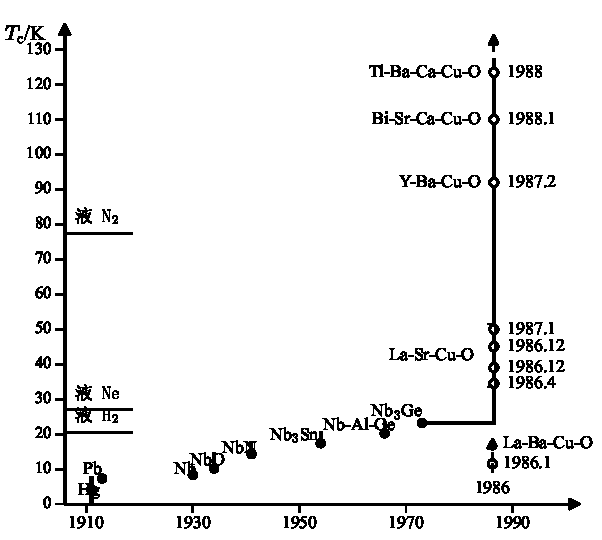
\includegraphics[width=7cm]{fig7-1.pdf}\\{\small 图 7.1\quad 超导转变温度提高的历史记录}
\end{minipage}
\end{center}

图7.1是超导转变温度提高的历史记录.显然，与1986年以前相比较，自从伯诺兹与穆勒新发现的铜氧化合物问世以来，超导转变温度屡破纪录，在不到两年的时间内 $T_{\mathrm{c}}$ 已提高了4～5倍，进入了便于工作的液氮温区，其临界磁场也很高（见表7.1），为超导电性的研究和应用开辟了一个新时期.因此，伯诺兹与穆勒在1986年的发现应当认为是超导电性研究的一个历史性的突破.正由于其贡献巨大，他们在一年之后就获得了1987年诺贝尔物理学奖.

迄今公认的最高超导转变温度也是朱经武研究组\textsuperscript{[8]}在 $\mathrm{HgBa}_{2}\mathrm{Ca}_{2}\mathrm{Cu}_{3}\mathrm{O}_{8+x}$（Hg-1223）化合物中测得的，其 $T_{\mathrm{c}}=133$ K，加压力甚至可使 $T_{\mathrm{c}}$ 提升到160 K以上.还应当指出，从1986年至今国内外还有很多更高 $T_{\mathrm{c}}$ 包括接近室温的报道，但可惜现象不稳定，样品难于重复或甚至不能重复，被朱经武教授戏称为“不明超导体”（unidentified superconducting objects，USO）\textsuperscript{[9]}.

值得一提的是，由于铜氧化合物高温超导体的 $T_{\mathrm{c}}$ 不断提高，反过来又启发和促进了常规超导体的研究.人们在 $\mathrm{C}_{60}$ 所组成的晶体中掺入足量的碱金属A（Cs、Rb等）使其金属化后，在 $\mathrm{A}_{3}\mathrm{C}_{60}$ 化合物中观测到转变温度 $T_{\mathrm{c}}$ 超过30 K的块体超导电性，属于电声子机制的BCS超导体，其中 $\mathrm{Cs}_{x}\mathrm{Rb}_{y}\mathrm{C}_{60}$ 的 $T_{\mathrm{c}}=33$ K（1991），而加压后的 $\mathrm{Cs}_{3}\mathrm{C}_{60}$（1995）$T_{\mathrm{c}}$ 可达到40 K\textsuperscript{[10]}.2000年美国巴特洛格（Batlogg）研究组在 $\mathrm{C}_{60}$ 晶体表面生长氧化层，设计了 $\mathrm{C}_{60}$ 的场效应三极管，通过调节系统的门电压可分别在 $\mathrm{C}_{60}$ 表层诱生电子或空穴，从而构成了一种载流子浓度可从电子型连续调节到空穴型的“掺杂”（不是化学掺杂，而是表面注入电子或空穴）$\mathrm{C}_{60}$ 金属系统，并发现当每个 $\mathrm{C}_{60}$ 中注入3～3.5个空穴时最高的 $T_{\mathrm{c}}$ 可达到52 K，而表层注入电子时最高 $T_{\mathrm{c}}$ 只有10 K.人们认为这是由于电子注入 $\mathrm{C}_{60}$ 的导带，空穴注入价带，而价带的能带电子态密度远远高于导带，相应的价带电声子互作用更强，导致空穴型 $\mathrm{C}_{60}$ 的 $T_{\mathrm{c}}$ 更高，但应注意在这里超导配对发生在 $\mathrm{C}_{60}$ 晶体的表面层，属于准二维系统的电声子机制超导电性（见文献\textsuperscript{[11]}中 Nature 杂志）.巴特洛格研究组在 $\mathrm{C}_{60}$ 分子间插入 $\mathrm{CHBr}_{3}$ 组成 $\mathrm{C}_{60}/\mathrm{CHBr}_{3}$ 的复合晶格，可使晶格常数从纯 $\mathrm{C}_{60}$ 的1.415 nm扩大为1.445 nm，随着晶格常数的增大，$\mathrm{C}_{60}$ 间载流子的近邻跃迁将减小，从而使能带变窄和态密度增加.根据最近的报道，他们发现当采用扩大的晶格 $\mathrm{C}_{60}/\mathrm{CHBr}_{3}$ 表面层做场效应三极管时，超导转变温度可提升到 $T_{\mathrm{c}}=117$ K，并声称如果 $\mathrm{C}_{60}$ 中再掺入适量的碱金属，$T_{\mathrm{c}}$ 还可以进一步升高（见文献\textsuperscript{[11]}中 Science 杂志），这是一个令人振奋的信息.另一个引人注目的进展是，2001年初在金属间化合物 $\mathrm{MgB}_{2}$\textsuperscript{[12]}中又发现了 $T_{\mathrm{c}}=39$ K 的块体超导电性，并已证实是电声子机制的常规超导体，它比同类二元金属间化合物 $\mathrm{Nb}_{3}\mathrm{Ge}$ 的 $T_{\mathrm{c}}$ 提高了近12 K，若进行掺杂还可以使 $\mathrm{MgB}_{2}$ 系统的 $T_{\mathrm{c}}$ 进一步提高.$\mathrm{C}_{60}$ 系列和 $\mathrm{MgB}_{2}$ 的发现突破了常规超导体的 $T_{\mathrm{c}}$ 一般不超过30 K的传统信念，引起了人们的极大兴趣，已成为当前超导电性研究的热点问题.

\section{结构与相图的共同特征}

\subsection*{1. 存在$\mathrm{CuO}_{2}$导电层——铜氧化合物结构的共同特征}

利用衍射技术可以确定新发现的铜氧化合物高温超导体的晶体结构.图7.2是两种典型氧化物超导体的结构示意，其中图(a)与图(b)分别代表 $\mathrm{La}_{2-x}\mathrm{Sr}_{x}\mathrm{CuO}_{4}$（La-214）和 $\mathrm{YBa}_{2}\mathrm{Cu}_{3}\mathrm{O}_{6+x}$（Y-123）的结构.图7.3为Bi系化合物（包括 Bi-2201，Bi-2212 和 Bi-2223）的结构.

\begin{center}
\begin{minipage}{6.5cm}
\centering
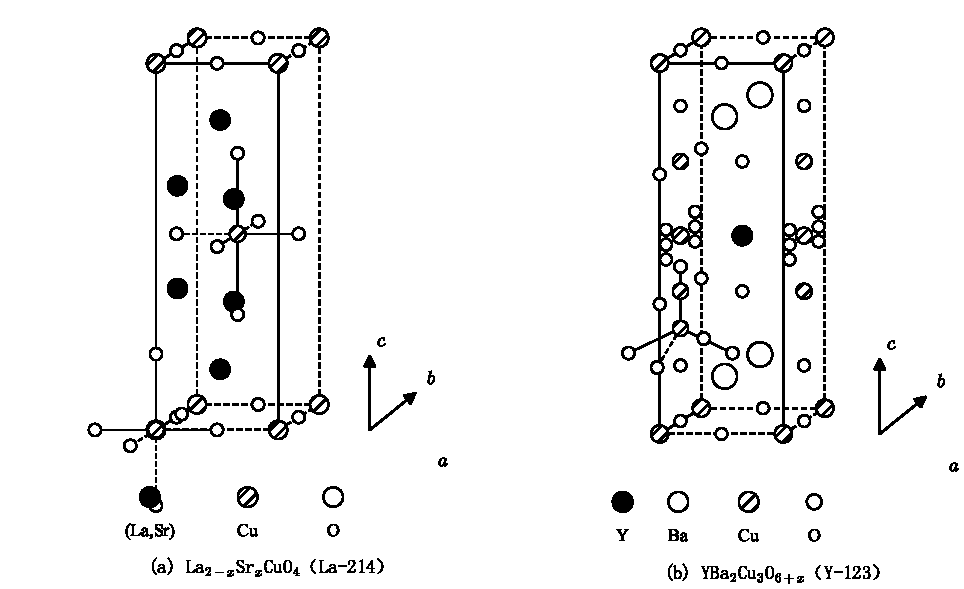
\includegraphics[width=6.5cm]{fig7-2.pdf}\\[0.3em]
{\small (a) $\mathrm{La}_{2-x}\mathrm{Sr}_{x}\mathrm{CuO}_{4}$（La-214）\qquad\qquad (b) $\mathrm{YBa}_{2}\mathrm{Cu}_{3}\mathrm{O}_{6+x}$（Y-123）}\\[0.2em]
{\small 图 7.2\quad 两种典型的氧化物高温超导体结构}
\end{minipage}
\end{center}

这些结构均具有正交对称性，其c轴方向的晶格常数大于a和b方向，是 $c>b\approx a$ 的近四方结构，它们基本上属于钙钛矿结构的变型.值得注意的是，在这些结构中均含有 $\mathrm{CuO}_{2}$ 平面层.例如在 La-214 与 Bi-2201 中只含一个 $\mathrm{CuO}_{2}$ 平面层，在 Y-123 和 Bi-2212 中含有两个 $\mathrm{CuO}_{2}$ 层，而在 Bi-2223 中则含3层，具有 $T_{\mathrm{c}}=125$ K 的 Tl-2223 和 $T_{\mathrm{c}}=133$ K 的 Hg-1223 结构也含有3层 $\mathrm{CuO}_{2}$ 平面.

\begin{center}
\begin{minipage}{6.5cm}
\centering
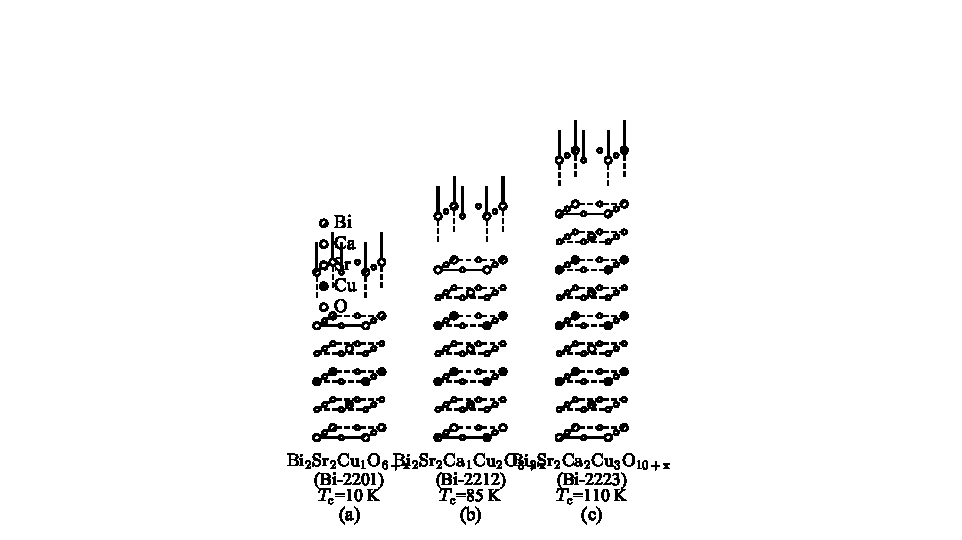
\includegraphics[width=6.5cm]{fig7-3.pdf}\\{\small 图 7.3\quad Bi系氧化物超导体的结构}
\end{minipage}
\end{center}

大量实验证据表明，这些氧化物高温超导体均具有平面导电特性，并且载流子运动主要是在 $\mathrm{CuO}_{2}$ 平面之中.能带计算也证实，系统的能带结构在费密面附近基本上不随 $k_{z}$（即垂直于 $\mathrm{CuO}_{2}$ 层方向波矢）变化，具有明显的二维特征，而且主要是来自 $\mathrm{CuO}_{2}$ 层中的电子能带贡献.另外，$\mathrm{CuO}_{2}$ 层内的 Cu 与 O 的键距也明显小于在c方向的键距，可将晶体看作为层状化合物，其中的 $\mathrm{CuO}_{2}$ 层可近似看作二维正方晶格.人们对于 $\mathrm{CuO}_{2}$ 层的作用进行了深入和集中的研究，获得了如下的主要结论：

(i) $\mathrm{CuO}_{2}$ 层对超导电性的产生起主要作用，这些层是铜氧化合物中的主要导电层，可称为导电单元.在这些化合物中的其它部分可以简单地看成是另一个结构单元，其主要作用是为导电单元（$\mathrm{CuO}_{2}$ 面或 $\mathrm{CuO}_{2}$ 面群）提供载流子，又可称为电荷库单元或简称电荷库（charge reservoir）.例如在 $\mathrm{La}_{2-x}\mathrm{Sr}_{x}\mathrm{CuO}_{4}$ 中，隔开相邻 $\mathrm{CuO}_{2}$ 导电层的两个（La，Sr）-O 层称为 La-214 的电荷库.又如在 $\mathrm{YBa}_{2}\mathrm{Cu}_{3}\mathrm{O}_{6+x}$ 结构中，导电单元由两层 $\mathrm{CuO}_{2}$ 平面组成，这两个 $\mathrm{CuO}_{2}$ 平面被Y原子平面所隔开，而当 $x=1$ 时 Y-123 的电荷库单元由（Ba-O)面-（Cu-O)键-（Ba-O)面组成，其中 Cu-O 链沿 b 轴方向，如图7.2(b)所示.当改变氧含量x时，$\mathrm{O}^{2-}$ 离子的含量主要是在 Cu-O 链所构成的平面中发生变化（从 $x=0$ 时，$\mathrm{YBa}_{2}\mathrm{Cu}_{3}\mathrm{O}_{6}$ 中不存在 Cu-O 链变化为，$x=1$ 时，$\mathrm{YBa}_{2}\mathrm{Cu}_{3}\mathrm{O}_{7}$ 中全为 Cu-O 链），它对导电层中的载流子浓度起调节作用.在 Bi-2223 中，由3个 $\mathrm{CuO}_{2}$ 平面（被Ca原子平面隔开）构成导电单元，而电荷库单元则含有一个 Sr-O 层和两个相互错位的 Bi-O 平面层（简称 Bi-O 双面），后者在氧含量改变时也对导电单元中的载流子浓度起调节作用.在 Bi-2212 中也存在调节载流子浓度的 Bi-O 双面.

(ii)根据以上讨论，复杂的铜氧化合物可以简化为两类结构单元，其中之一是导电单元或导电层，由1～3层 $\mathrm{CuO}_{2}$ 平面堆积而成.在两相邻导电单元之间的其余部分笼统称作电荷库.为了便于利用导电层与电荷库之间的电荷转移模型来说明掺杂，增氧或脱氧是如何调节 $\mathrm{CuO}_{2}$ 导电层中的载流子浓度，可以将含有单层、双层和3层 $\mathrm{CuO}_{2}$ 面的 La-214、Y-123 及 Bi-2223 等氧化物系统的结构单元形象地图示为：

\begin{center}\small
\begin{tabular}{ll}
\underline{单层系} & \rule[-0.3ex]{3.2cm}{0.4pt}\quad 导电层\quad $\mathrm{CuO}_{2}$面\\
$\mathrm{La}_{2-x}\mathrm{Sr}_{x}\mathrm{CuO}_{4}$ & \\
（La-214，$T_{\mathrm{c}}=40$ K） & \quad\fbox{电荷库}\\
$\mathrm{Bi}_{2}\mathrm{Sr}_{2}\mathrm{CuO}_{6+x}$ & \rule[-0.3ex]{3.2cm}{0.4pt}\quad 导电层\quad $\mathrm{CuO}_{2}$面\\
（Bi-2201，$T_{\mathrm{c}}=10$ K） & \\
\underline{双层系} & \rule[-0.3ex]{3.2cm}{0.4pt}\\
 & \rule[-0.3ex]{3.2cm}{0.4pt}\quad $\mathrm{CuO}_{2}$面群\\
$\mathrm{YBa}_{2}\mathrm{Cu}_{3}\mathrm{O}_{6+x}$（$x\to1$） & \quad\fbox{电荷库$\left(\begin{array}{c}\mbox{Cu-O 链或}\\ \mbox{Bi-O 双面}\end{array}\right)$}\\
（Y-123，$T_{\mathrm{c}}=90$ K） & \\
$\mathrm{Bi}_{2}\mathrm{Sr}_{2}\mathrm{CaCu}_{2}\mathrm{O}_{8}$ & \rule[-0.3ex]{3.2cm}{0.4pt}\\
（Bi-2212，$T_{\mathrm{c}}=85$ K） & \rule[-0.3ex]{3.2cm}{0.4pt}\quad $\mathrm{CuO}_{2}$面群\\
\underline{3层系} & \rule[-0.3ex]{3.2cm}{0.4pt}\\
 & \rule[-0.3ex]{3.2cm}{0.4pt}\\
 & \rule[-0.3ex]{3.2cm}{0.4pt}\quad 导电层\\
$\mathrm{Bi}_{2}\mathrm{Sr}_{2}\mathrm{Ca}_{2}\mathrm{Cu}_{3}\mathrm{O}_{10+x}$ & \quad\fbox{电荷库（含 Bi-O 双面）}\\
 & \rule[-0.3ex]{3.2cm}{0.4pt}\\
 & \rule[-0.3ex]{3.2cm}{0.4pt}\\
（Bi-2223，$T_{\mathrm{c}}=110$ K） & \rule[-0.3ex]{3.2cm}{0.4pt}\quad 导电层\\
\end{tabular}
\end{center}

(iii)为了定性说明掺杂如何控制导电层中载流子浓度，继续采用表格形式描述在 La-214 中掺入 Sr 原子时载流子浓度的变化过程：

\begin{center}\small
\begin{tabular}{lll}
 & & \rule[-0.3ex]{2.0cm}{0.4pt}\ $\mathrm{CuO}_{2}$：$\mathrm{Cu}^{2+}(\mathrm{O}^{2-})_{2}$\\
$\mathrm{La}_{2}\mathrm{CuO}_{4}$ & & \\
$\downarrow$ & 电荷库 & \quad\rule[-0.3ex]{1.4cm}{0.4pt}\ $\mathrm{LaO}$：$\mathrm{La}^{3+}\mathrm{O}^{2-}$\\
（掺Sr） & & \quad\rule[-0.3ex]{1.4cm}{0.4pt}\ $\mathrm{LaO}$：$\mathrm{La}^{3+}\mathrm{O}^{2-}$\\
$\downarrow$ & & \rule[-0.3ex]{2.0cm}{0.4pt}\ $\mathrm{Cu}^{2+}(\mathrm{O}^{2-})_{2}+x\,|e|$\\
$\mathrm{La}_{2-x}\mathrm{Sr}_{x}\mathrm{CuO}_{4}$ & 电荷库 & \quad\rule[-0.3ex]{1.4cm}{0.4pt}\ $\mathrm{La}^{3+}_{1-x/2}(\mathrm{Sr}^{2+})_{x/2}\mathrm{O}^{2-}_{4}$\\
 & & \quad\rule[-0.3ex]{1.4cm}{0.4pt}\ $\mathrm{La}^{3+}_{1-x/2}(\mathrm{Sr}^{2+})_{x/2}\mathrm{O}^{2-}_{4}$\\
\end{tabular}
\end{center}

首先必须明白，在 La-214 中 Sr 是掺入到电荷库中的两个 La-O 平面上的，当掺杂浓度为 x 时，在两个 La-O 平面上La的芯态总共缺少x浓度的电子，而且其芯态的能级又低于费密能级，所以位于费密能级附近的 $\mathrm{CuO}_{2}$ 导电层的二维能带中的电子可以向电荷库转移，从而使导电层中含有x浓度的空穴型载流子.这就是La-214中掺杂改变电荷库，转而控制 $\mathrm{CuO}_{2}$ 导电层中载流子浓度的具体过程.利用上述电荷转移机制还可以说明铜氧化物中既有空穴型，又有电子型超导体.这是因为在La基化合物中，当人们用2价的 Sr 取代3价的 La 时，由于电荷库中缺少电子，必将在 $\mathrm{CuO}_{2}$ 导电层中产生空穴.反过来，在Nd基化合物中掺入4价的 Ce 用以取代3价的Nd时，自然在电荷库中会多出电子，从而使 $\mathrm{CuO}_{2}$ 导出层中的载流子变为电子.因此，$\mathrm{La}_{2-x}\mathrm{Sr}_{x}\mathrm{CuO}_{4}$ 是空穴型，而 $\mathrm{Nd}_{2-x}\mathrm{Ce}_{x}\mathrm{CuO}_{4}$ 则是电子型的氧化物超导体，此结论已被霍尔系数的测量所证实.

关于改变氧含量对导电层中载流子浓度的影响，应以Y-123为例作说明.在 $\mathrm{YBa}_{2}\mathrm{Cu}_{3}\mathrm{O}_{6+x}$（$0\leqslant x\leqslant1$）中，对于Cu-O链上的氧原子实验已证实它是很容易进出的，因此氧含量的增加或减少（即增氧与脱氧）应首先发生在电荷库中的 Cu-O 链上.当有x浓度的氧原子从体外的零价态氧原子变成链上的 $\mathrm{O}^{2-}$ 离子时，将导致库中缺少2x个电子，其中的一半来自链上的铜处于+1价态 $\mathrm{Cu}^{+}$，另一半的电子则主要是通过电荷转移从导电层进入电荷库，这就使得 $\mathrm{CuO}_{2}$ 导电层中出现相应的空穴浓度.简言之，在Y-123中当氧含量增加到 $6+x$ 时，将在 $\mathrm{CuO}_{2}$ 导电层中产生x浓度的空穴，这些空穴基本上处在 $\mathrm{CuO}_{2}$ 面的氧位上，而不是靠近层中的 $\mathrm{Cu}^{2+}$ 位形成3价态的 $\mathrm{Cu}^{3+}$ 离子.在Bi基化合物的电荷库中，Bi-O 双面起作 Y-123 中 Cu-O 链的类似作用，它也是通过改变电荷库中的氧含量来调节 $\mathrm{CuO}_{2}$ 导电层中的空穴浓度.

\subsection*{2. 存在绝缘性的反铁磁母体化合物——相图的共同特征}

所有新发现的铜氧化合物高温超导体都可以认为是由某些母体化合物经掺杂或改变氧含量形成的，而这些化合物均是反铁磁绝缘体（AFI）.对于掺杂的 La-214（$\mathrm{La}_{2-x}\mathrm{Sr}_{x}\mathrm{CuO}_{4}$）、Nd-214（$\mathrm{Nd}_{2-x}\mathrm{Ce}_{x}\mathrm{CuO}_{4}$）以及改变氧含量的 Y-123（$\mathrm{YBa}_{2}\mathrm{Cu}_{3}\mathrm{O}_{6+x}$）等超导体的母体化合物，中子衍射实验已证实它们均是反铁磁绝缘体，其反铁磁奈耳（Neel）温度为
\begin{equation*}
\begin{aligned}
&\text{La-214（$x=0$）：}\mathrm{La}_{2}\mathrm{CuO}_{4}\,,\ T_{\mathrm{N}}=300\ \mathrm{K}\\
&\text{Y-123（$x=0$）：}\mathrm{YBa}_{2}\mathrm{Cu}_{3}\mathrm{O}_{6}\,,\ \ T_{\mathrm{N}}=460\ \mathrm{K}\\
&\text{Nd-214（$x=0$）：}\mathrm{Nd}_{2}\mathrm{CuO}_{4}\,,\ T_{\mathrm{N}}=250\ \mathrm{K}
\end{aligned}
\end{equation*}
此外，在Bi和Tl的铜氧化物高温超导体中，若用Y置换Ca也呈现磁性相.因此，存在绝缘性的反铁磁母体化合物是高温超导体的另一共性特征.

应特别注意的是，上述母体化合物都是绝缘体而不是金属，这是涉及铜氧化物体系的一个新特点.根据能带理论，在独立电子近似下，这些母体化合物中靠近费密面的铜3d带应当是半填满的，它们似乎应表现出金属性，但是中子衍射实验中所观测到的都不是金属，而是反铁磁绝缘体.在理论上要解释这一矛盾，必须将铜氧化合物当作强关联电子体系处理，即必须超出独立电子近似，计入在同一格点周围自旋取向相反电子间的强库仑关联（又称“同位”库仑关联）.在第十一章中，我们将引入赫伯德（Hubbard）模型描述强关联电子体系，并证明，在强关联极限下，半满赫伯德模型的严格基态是绝缘体，而非金属.因此，在母体化合物中观测到反铁磁绝缘体的事实已经提供了这类铜氧化合物属于强关联电子体系的证据.进一步的实验与理论研究结果还表明，在 $\mathrm{CuO}_{2}$ 层体系中存在着很强的层内交换作用（见第十一章§9）和比较弱的层间耦合，前者代表 $\mathrm{CuO}_{2}$ 平面内近邻Cu格点间的交换作用J（约为 $10^{3}\sim10^{4}$ K），它是体系中的主要相互作用，后者则是被电荷库单元所隔开的导电层的层间耦合，它导致在母体化合物中形成三维的反铁磁长程序.由于层间耦合远远小于层内交换作用，因此观测到的反铁磁奈耳温度 $T_{\mathrm{N}}$（$T_{\mathrm{N}}$ 约为 $10^{2}$ K）都比层内反铁磁交换作用J所对应的温度低1～2个数量级.这一特点又表明，铜氧化物高温超导体可以看作是准二维的强关联电子体系.

为了使读者对氧化物高温超导体的相图有比较具体的了解，我们在图7.4中给出 $\mathrm{La}_{2-x}\mathrm{Sr}_{x}\mathrm{CuO}_{4}$ 的相图，其中纵轴代表温度T，横轴则由 Sr 的掺杂浓度x表示，并认为x大致上是单位 $\mathrm{CuO}_{2}$ 层的空穴浓度.显然，未掺杂（$x=0$）时的母体化合物 $\mathrm{La}_{2}\mathrm{CuO}_{4}$ 为反铁磁绝缘体.经掺杂，$T_{\mathrm{N}}$ 急剧下降，当空穴浓度x达到0.01～0.02时反铁磁长程序消失（$T_{\mathrm{N}}=0$），系统过渡到只有短程磁序的绝缘相，通常称为自旋液体.当 $x\approx0.05$ 时，发生绝缘体-金属相变，系统进入金属相并在 $T<T_{\mathrm{c}}$ 时呈现出超导电性，其最高超导转变温度 $T_{\mathrm{c}}$ 为40 K，位于 $x=0.15\sim0.2$ 范围内，而在 $T_{\mathrm{c}}$ 以上的正常态则具有一系列不同于普通金属的异常特性，涉及强关联电子体系的非费密液体（NFL）行为，可简称为强关联金属.继续掺杂，当 $x>0.3$ 时，高温超导电性消失，系统进入正常费米液体状态，才可称为正常金属态.此外，还存在着一个从高温到低温的四方-正交结构相变.Y-123 与 Tl-2223 等氧化物高温超导体的相图均类似于La-214的相图.按此，可取T为纵轴，用掺杂程度作为横轴，将氧化物高温超导体相图的共同特征粗线条地归纳为一个简单、而且通用的定性相图，如图7.5所示.从这个定性的通用相图，人们不难得知如下信息：

\begin{center}
\begin{minipage}{8cm}
\centering
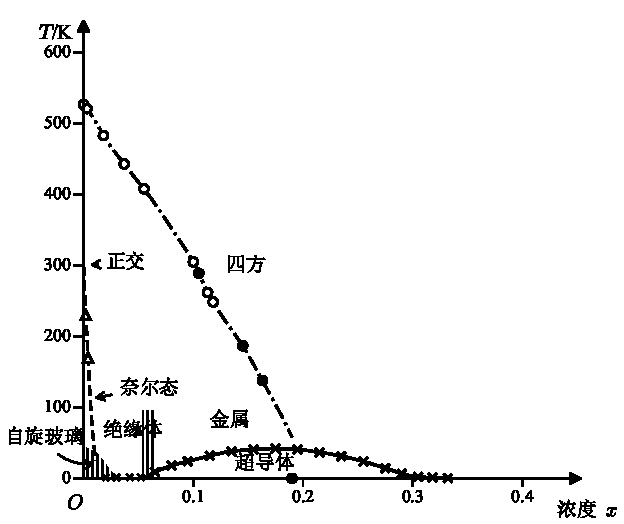
\includegraphics[width=8cm]{fig7-4.pdf}\\{\small 图 7.4\quad $\mathrm{La}_{2-x}\mathrm{Sr}_{x}\mathrm{CuO}_{4}$ 的相图}
\end{minipage}
\end{center}

\begin{center}
\begin{minipage}{8.5cm}
\centering
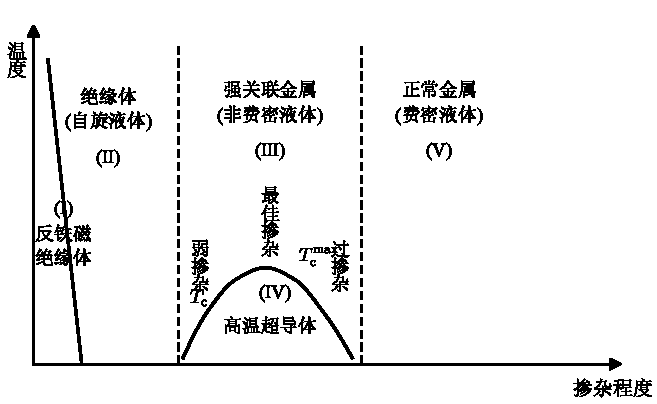
\includegraphics[width=8.5cm]{fig7-5.pdf}\\{\small 图 7.5\quad 氧化物高温超导体的通用相图}
\end{minipage}
\end{center}

(i)母体化合物通常为反铁磁绝缘体，出现在（Ⅰ)区中.

(ii)反铁磁长程序对掺杂极为敏感，当掺杂时反铁磁性迅速消失，取而代之的是高度关联的自旋液体（Ⅱ).

(iii)经绝缘体-金属（I-M）转变，系统进入强关联金属区（Ⅲ)，其特征往往不能用标准的费密液体理论解释.中子衍射实验表明I-M转变对自旋关联并无明显的影响，说明在强关联金属中仍然存在反铁磁自旋关联.

(iv)从强关联金属区域（Ⅲ)降温，系统才能进入高 $T_{\mathrm{c}}$ 超导态区域（Ⅳ).实验还表明，反铁磁自旋关联将一直延伸到高 $T_{\mathrm{c}}$ 超导态中.

(v)进一步掺杂，系统最终进入正常金属区（V)，其特征可用标准费密液体理论中描述，但降温时却不再出现超导电性了.

常规的BCS超导体与氧化物高温超导体最重要的区别在于，BCS超导体的正常态为费密液体，而高 $T_{\mathrm{c}}$ 超导体的正常态为非费密液体.近年来的研究还表明强关联金属区域（Ⅲ)又分为3个区，其中对应于最高转变温度 $T_{\mathrm{c}}$ 的掺杂称为最佳掺杂，掺杂量大于或小于这一数值，分别称为过掺杂与弱掺杂（或欠掺杂），而在这3个区域中正常态的行为有很大的差别，表现在弱掺杂区中出人意料地发现了正常态的能隙，仅当掺杂浓度增加，系统进入最佳掺杂和过掺杂区时，这种异常现象才消失.现已明白，存在正常态能隙是所有铜氧化合物高温超导体在弱掺杂区的普遍特征（详见本章§8），这对理论研究提出了新的挑战.时至今日，如何理解氧化物高 $T_{\mathrm{c}}$ 材料的相图共同特征仍是摆在理论工作者面前的一项基本任务.要建立一个铜氧化合物的超导理论，其主要任务不仅限于解释高 $T_{\mathrm{c}}$ 出现的原因，还应当对上述通用相图（包括弱掺杂区出现正常的能隙）作出全面的解释，这是一个相当高的要求.近年来出现的高温超导电性的SO(5)理论\textsuperscript{[14]}，在研究反铁磁性与高 $T_{\mathrm{c}}$ 超导电性的统一描述方面迈出了重要的一步，值得读者关注.

\section{高温超导体中超导态的基本属性}

在本节中，我们将介绍铜氧化合物超导态的主要特征，并着重于讨论它与BCS超导态的不同之处.

在新发现的铜氧化物高温超导体中，由于对超导配对和正常态输运起关键作用的载流子处于 $\mathrm{CuO}_{2}$ 导电层内，而且这些超导体都具有以 $\mathrm{CuO}_{2}$ 平面为主体的层状结构，普遍认为这些高温超导体的主要物理性质应大致相同.基于这一共识，科学家们将注意力集中于研究某些典型的材料，例如Y-123，因为这类化合物便于制成均匀、纯净和足够大尺寸的单晶，可供标定样品的内在特性.随着样品质量的不断提高和测量手段的不断改进，来自不同研究组的测量数据越来越集中且可靠，对于Y-123甚至达到了彼此定量一致的程度，从而为正确理解高 $T_{\mathrm{c}}$ 铜氧化合物的超导态和正常态属性提供了可靠的依据.对于超导态的基本物理性质，目前已取得共识的主要结果是：

\subsection*{1. 超导态仍然是库柏对的相干凝聚态}

在高温超导体被发现后，随即在诸多的实验中（包括：交流约瑟夫森效应、磁通跳跃、Little-Parks振荡以及磁通量子的直流测量等）均证实了传载超电流的有效电荷为 $e^{*}=2e$\textsuperscript{[15]}，这表明不论是空穴型的、还是电子型的高温超导体仍然是由两个载流配对组成的凝聚体.安德列耶夫（Andreev）反射实验更进一步证实了配对的载流子具有相反的动量和自旋，这与BCS超导态相似，仍然是由（$k\uparrow$）与（$-k\downarrow$）载流子组成的自旋单重态配对——库柏对，而在超导态中传递超电流的有效单元仍应是相位相干的，并已形成了凝聚的库柏对系统，但配对与相干凝聚未必同时发生，也正是在这个意义上我们说，超导仍然是（$k\uparrow$，$-k\downarrow$）载流子对总体的相干凝聚.

人们自然要问及，当高温超导体进入超导状态以后，超导能隙函数的对称性，它涉及超导态的另一个重要特性.

\subsection*{2. 配对的对称性——主要是各向异性的d波配对}

超导能隙函数在物理上代表传递超电流的载流子对（即电子对-电子型，或空穴对-空穴型超导体）波函数的轨道部分，又称超导序参量.由于实验已证实在高温超导体中波函数的自旋部分仍然是奇宇称的自旋单重态，根据全同性原理，能隙函数只能是动量空间中取向 $\hat{\boldsymbol{k}}$ 的偶函数，对应于用球谐函数 $\mathrm{Y}_{lm}(\boldsymbol{k})$ 展开的对波函数轨道部分中取 $l=0,\ 2,\ \cdots$ 等偶宇称解，其中 $l=0$ 情形称为s波配对的各向同性BCS超导体，而 $l=2$ 则称为d波配对的各向异性超导体（在§4将作专门的介绍）.对于BCS超导体，能隙函数在费密面上各方向均取相同的数值 $\Delta$，属于各向同性的s波情形，其中 $2\Delta$ 代表在超导态中折开一个库柏对所需的最小能量，而产生单个准粒子激发所需最小能量为 $\Delta$.由此可知，在BCS超导态中的低温（$T\ll T_{\mathrm{c}}$）元激发密度应与 $\exp(-\beta\Delta)$ 成正比，其中 $\beta=1/k_{\mathrm{B}}T$.当人们测量BCS超导体中的比热容系数和伦敦穿透深度等与元激发密度有关的物理量时，它们在低温下均呈现指数型的温度依赖关系 $\exp(-\beta\Delta)$，这是BCS超导体的一个标志性特征.

对于具有临界温度为40 K以上的各向异性铜氧化合物，为了判断其超导序参量的对称性，至少应当区分下列3种配对，它们分别是：各向同性的s波，$d_{x^{2}-y^{2}}$ 波和各向异性的s波配对，它们在实空间的示意图如图7.6所示.

\begin{center}
\begin{minipage}{8.5cm}
\centering
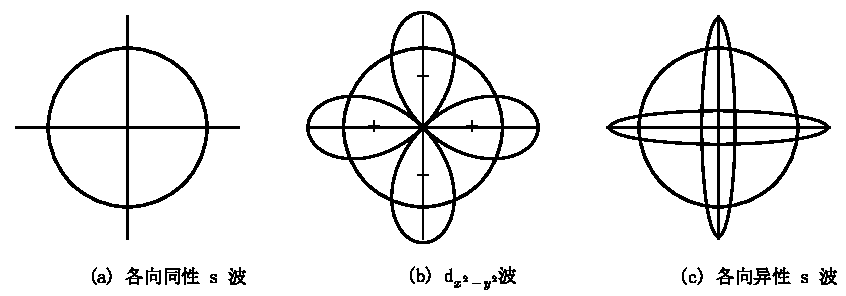
\includegraphics[width=8.5cm]{fig7-6.pdf}\\[0.3em]
{\small (a) 各向同性s波\qquad\quad (b) $d_{x^{2}-y^{2}}$波\qquad\quad (c) 各向异性s波}\\[0.2em]
{\small 图 7.6\quad 超导序参量在实空间中的示意图}
\end{minipage}
\end{center}

早期的实验似乎支持s波图像，包括各向同性的s波［如(a)所示］以及反映超导晶体对称性的各向异性s波配对［如(c)所示］，其中序参量是随着取向变化的，但是序参量的对称性不低于晶体的对称性，仍属于常规s波情形.另一方面，理论工作者也早已提出了 $d_{x^{2}-y^{2}}$ 波配对方案，这是考虑到在 $\mathrm{CuO}_{2}$ 平面内 Cu 的 $d_{x^{2}-y^{2}}$ 轨道电子起主要作用，并且在同一个Cu格点上电子间存在强的同位库仑排斥作用，由于d波配对在粒子间距很小时，对波函数的概率幅也很小，有利于避开高 $T_{\mathrm{c}}$ 氧化物中普遍存在的强同位库仑排斥（简称强关联）作用而形成配对.$d_{x^{2}-y^{2}}$ 波的序参量大小随取向变化，在 $Oxy$ 平面上为四叶草（four-leaf clover）形状，但是 $d_{x^{2}-y^{2}}$ 波不同于各向异性s波的关键性特征是，具有两个正叶和两个负叶，它们的最大数值分别沿x轴和y轴方向，并且沿对角线（$|x|=|y|$ 方向）经过零点，与此同时序参量改变符号，如图7.6(b)所示，各向异性s波的序参量则没有符号的改变，其四个叶瓣均为正，而且沿对角线方向尽管数值很小，但仍为非零，即存在一个最小的实能隙.从对称性分析看，各向异性s波的序参量仍具有超导晶体的4次轴对称，但是 $d_{x^{2}-y^{2}}$ 波（由于存在正、负叶）则无此对称性，其超导序参量的对称性低于超导晶体，被称为非常规配对情形.在动量空间中，超导序参量代表费密面上的能隙函数 $\Delta(\hat{\boldsymbol{k}})$，其中 $\hat{\boldsymbol{k}}\equiv\boldsymbol{k}/\left|\boldsymbol{k}\right|$ 代表沿 k 方向的单位矢量.在二维BZ中，$d_{x^{2}-y^{2}}$ 波的能隙函数可表示为
\begin{equation}
  \Delta(\hat{\boldsymbol{k}})\sim\left(\hat{k}_{x}^{2}-\hat{k}_{y}^{2}\right)=\cos2\phi_{k}\,,\qquad
  \phi_{k}=\arctan\left(\hat{k}_{y}/\hat{k}_{x}\right)
\end{equation}
它不仅随k的取向变化，而且与实空间序参量特性相似，在k空间的某些区域 $\Delta$ 为正，另一些区域 $\Delta$ 为负，沿 $k_{x}$ 和 $k_{y}$ 方向分别取正和负的最大值，并且沿 $|k_{x}|=|k_{y}|$ 方向经过 $\Delta(\hat{\boldsymbol{k}})$ 的零点.能隙函数改变符号和存在零点是 $d_{x^{2}-y^{2}}$ 波配对区别于各向异性s波配对的重要特点.因此，必须直接测量能隙函数 $\Delta(\hat{\boldsymbol{k}})$ 随取向 $\hat{\boldsymbol{k}}$ 的变化，才能从实验上对高温超导体中是否存在非常规的 $d_{x^{2}-y^{2}}$ 波配对作出明确的判断.

角分辨光发射谱仪（ARPES）是一个可以直接测量能隙随取向 $\hat{\boldsymbol{k}}$ 变化的重要手段.1993年斯坦福大学研究组\textsuperscript{[16]}首先发现，在 Bi-Sr-Ca-Cu-O（BSCCO）化合物中，沿 $k_{x}$ 或 $k_{y}$ 方向能隙取最大值，而沿对角线 $|k_{x}|=|k_{y}|$ 方向所测出的能隙值非常小，甚至可以认为是零，具有类似 $d_{x^{2}-y^{2}}$ 波的四叶草形状.类似的结果也在 Y-Ba-Cu-O（YBCO）等化合物中被观测到，但是ARPES测量只能给出沿某个方向能隙的数值 $\left|\Delta(\hat{\boldsymbol{k}})\right|$，而不能辨别能隙的符号取正值还是负值.在这个意义上讲，他们的发现仅仅证明了超导能隙函数是各向异性的，但仍然无法区别 $d_{x^{2}-y^{2}}$ 波和各向异性s波配对，因此，人们又将注意力转向对于能隙 $\Delta$ 的符号改变十分敏感的约瑟夫森结实验.应当明白，超导能隙函数 $\Delta$ 改变符号时，作为一个复序参量函数，相当于 $\Delta$ 的相位改变 $180^{\circ}$，即有相移 $\pi$，人们必须设计出一种能够观测超导序参量相位变化的实验系统.

在相位观测方面，伊利诺斯大学的哈林根（D. V. Harlingen）等人\textsuperscript{[17]}首先作出了贡献，他们用一块常规的BCS超导体铅（Pb）和一块高质量的YBCO单晶做成含有两个约瑟夫森结的超导量子干涉系统，其中各向同性s波超导体 Pb 的两端分别与高温超导体 YBCO 单晶的两个相互垂直的晶面相接触构成约瑟夫森结，组合的构形可参考图7.7(a).如果YBCO也是s波配对，这一组合将不会引入附加的相位差，只能观察到通常的双结量子干涉效应.然而，当YBCO具有 $d_{x^{2}-y^{2}}$ 波对称性时，则将在平行于x（或a）轴的结中出现d波态超导序参量的负叶，而在平行于y（或b）轴的结中出现d波态的正叶，这时YBCO中的负叶将通过相位为各向同性的Pb超导体的连接，面对 YBCO 另一侧的正叶，导致两个结之间有 $\pi$ 相移.在无外磁场时，这一相移 $\pi$ 将使流经两个结的约瑟夫森超电流彼此相消.哈林根等人通过测量临界电流（即最大超电流）与外磁场的关系，在零外场时看到了临界电流的明显相消效应，这是支持d波配对的第一个实验证据.1995年，马里兰大学研究组\textsuperscript{[18]}改用薄膜，而不是块体，构造了与伊利诺斯小组相似的 YBCO-Pb 双结组合，即图7.7(a).他们采用扫描述磁强计直接测出 YBCO-Pb 组合环中的磁通 $\Phi$ 为半整的量子磁通 $\left(n+\dfrac{1}{2}\right)\Phi_{0}$，其中 $\Phi_{0}=\left(\pi\hbar c/e\right)$ 为磁通量子.在这里半个磁通量子 $\left(\dfrac{1}{2}\Phi_{0}\right)$ 的出现是由于 YBCO-Pb 环路中两垂直结之间存在d波相移 $\pi$.为了排除由于结面不平整或含有磁性杂质等偶然因素引起额外的磁通捕获、但却被误认为是d波序参量产生的相移而导致假象的半个磁通量子，马里兰研究组还同时设计了两个结平行于y（即b）轴的组合，如图7.7(b).显然，在(b)组合中两个平行结之间是不存在来自d波配对的相位差，也不会有半整数的量子磁通效应，威尔斯托德（Wellstood）等人在(b)组合中只观察到整数的磁通量子，从而排除了上述偶然因素的影响，与d波配对所预言的结果一致.特别值得一提的是IBM的崔（Tsuei）和克尔特勒（Kirtley）等人的工作\textsuperscript{[19]}，他们利用分子束外延方法首先制了成全由高温超导体YBCO薄膜组成的多结环，在结两侧的YBCO取向不同，可构成 YBCO 中 $d_{x^{2}-y^{2}}$ 配对的正叶直接面对结另一侧YBCO的负叶，形成相移，而无需通过BCS超导体铅作为中介，必然更直接地反映 YBCO 中序参量的对称性.1994年，他们在全由YBCO构成的三结环中首先观察到半个磁通量子的捕获，直接证实了YBCO中为 $d_{x^{2}-y^{2}}$ 波配对，被人们誉为是证实高温超导体为d波配对的里程碑性工作.实验测量还进一步表明，不仅是YBCO，在 Tl-2201 和 BSCCO 等其它的一系列铜氧化物高温超导体中均已证实能隙函数的主导部分都是 $d_{x^{2}-y^{2}}$ 波配对，唯一的例外是电子型的 Nd-Ce-Cu-O 化合物，迄今的实验结果均表明它仍然属于常规的s波配对.

\begin{center}
\begin{minipage}{8cm}
\centering
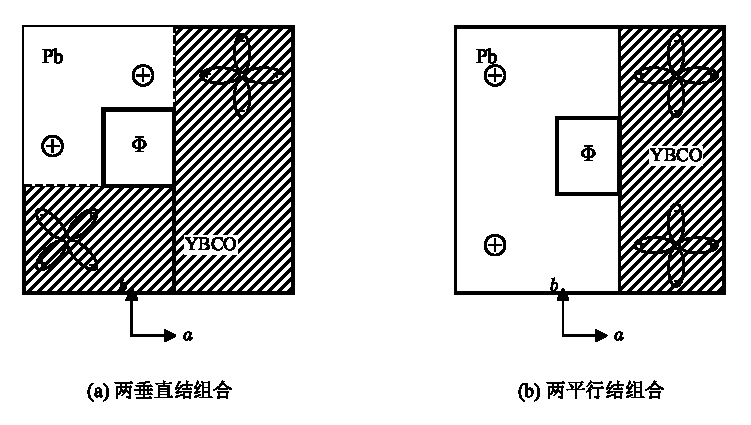
\includegraphics[width=8cm]{fig7-7.pdf}\\[0.3em]
{\small (a) 两垂直结组合\qquad\qquad (b) 两平行结组合}\\[0.2em]
{\small 图 7.7\quad YBCO-Pb 构成的超导量子干涉仪}
\end{minipage}
\end{center}

上面所说的以 $d_{x^{2}-y^{2}}$ 波为主导成分是指，由于实际超导体的配对对称性相当复杂，不排除可能有各向同性s波配对的附加贡献，从而形成混合的 s+d 配对.这类 s+d 混合配对已在YBCO中被观测到，并初步认定是由于各向同性的s波成分的混入，来源于YBCO中存在正交畸变，即当出现超导电性时实际上已是 $a\neq b\neq c$ 的正交晶体\textsuperscript{[20]}.对于不存在正交畸变的 BSCCO 和 Tl-2201 等超导体仍属纯 $d_{x^{2}-y^{2}}$ 波配对，它们的能隙函数都可用式(7.3.1)描述.

\subsection*{3. 极端的Ⅱ类超导体}

铜氧化物高温超导体的明显层状结构将直接影响其超导态中的电子性质，由于这类化合物可以看作为弱耦合 $\mathrm{CuO}_{2}$ 超导层的组合，将导致描述超导电性的参量（如磁穿透深度 $\lambda$ 和超导相干长度 $\xi$ 等）呈现出强烈的各向异性.表7.2中列出了3种氧化物高温超导体在平行于 $\mathrm{CuO}_{2}$ 面（ab平面）和垂直于 $\mathrm{CuO}_{2}$ 面（c方向）的 $\lambda$ 与 $\xi$ 值，其中的 $\xi$ 值是从上临界场 $H_{c2}$ 的测量推算出的G-L相干长度，表中还列出了典型的BCSⅡ类超导体的 $\lambda$ 与 $\xi$ 值，以兹比较.

表7.2\quad 氧化物高温超导体的零温磁穿透深度和G-L相干长度

\begin{center}\small
\begin{tabular}{lcccc}
\hline
化合物 & $\lambda_{ab}(0)$/nm & $\lambda_{c}(0)$/nm & $\xi_{ab}(0)$/nm & $\xi_{c}(0)$/nm\\
\hline
$\mathrm{La}_{2-x}\mathrm{Sr}_{x}\mathrm{CuO}_{4}$ & $800\times10^{-1}$ & $4\,000\times10^{-1}$ & $35\times10^{-1}$ & $7\times10^{-1}$\\
$\mathrm{YBa}_{2}\mathrm{Cu}_{3}\mathrm{O}_{7}$ & $1\,500\times10^{-1}$ & $6\,000\times10^{-1}$ & $15\times10^{-1}$ & $3\times10^{-1}$\\
$\mathrm{Bi}_{2}\mathrm{Sr}_{2}\mathrm{Ca}_{2}\mathrm{Cu}_{3}\mathrm{O}_{10}$ & $2\,000\times10^{-1}$ & $10\,000\times10^{-1}$ & $13\times10^{-1}$ & $2\times10^{-1}$\\
\hline
Nb（Ⅱ类BCS） & \multicolumn{2}{c}{$\lambda=350\times10^{-1}$ nm} & \multicolumn{2}{c}{$\xi=400\times10^{-1}$ nm}\\
\hline
\end{tabular}
\end{center}

除了强各向异性外，所有的氧化物高温超导体由于 $\xi(0)$ 很短，均属于Ⅱ类超导体，其G-L参数
\begin{equation}
  \kappa\equiv\left(\lambda/\xi\right)\gg1/\sqrt{2}
\end{equation}
其中 $1/\sqrt{2}$ 是Ⅱ类超导体的最小 $\kappa$ 值.对于高 $T_{\mathrm{c}}$ 超导材料，$\kappa$ 值超过100，而且由于它们的相干长度 $\xi$ 远远小于 $T_{\mathrm{c}}$ 附近的电子平均自由程 $\left[\left(100\sim200\right)\times10^{-1}\,\mathrm{nm}\right]$，它们是处于干净极限下的极端Ⅱ类超导体.

具体与BCS超导体相比较，氧化物高温超导体的磁穿透深度，即使在 $\mathrm{CuO}_{2}$ 平面内，也相对大一些，这是由于铜氧化合物中的载流子浓度偏低 $\left[n=\left(2\sim5\right)\times10^{21}\,\mathrm{cm}^{-3}\right]$，导致对外磁场屏蔽不足的必然结果.更为突出的是，垂直或平行于 $\mathrm{CuO}_{2}$ 面的相干长度 $\xi_{c}(0)$ 和 $\xi_{ab}(0)$ 比常规BCS超导体的 $\xi$ 要短得多，在氧化物材料中 $\xi(0)$ 的平均值仅为1 nm，和晶胞的尺寸同一量级，只有BCS超导体的1/100～1/10.如此短的平均相干长度 $\xi$，使氧化物高温超导体在相干体积（约 $\xi^{3}$）内只可能含有几个库柏对，与BCS超导体铝（Al）的相体积中有 $10^{4}$ 个库柏对相比较，低了几个数量级，这将使涨落效应变得十分突出.另外，考虑到这里的 $\xi(0)$ 实际上是零温时的G-L相干长度，根据第六章§10的讨论，它实际上代表外扰动所引起超导序参量（或能隙函数）的变化范围或衰减距离，而在铜氧化合物中这个距离很短，甚至单个外来原子也将可能在局部范围内压制掉超导能隙，这又说明高温超导体对于小尺寸的化学结构缺陷将是十分敏感的.

\subsection*{4. 复杂的同位素效应}

在BCS超导体中，同位素效应的实验结果为
\begin{equation}
  T_{\mathrm{c}}\sim M^{-\alpha}
\end{equation}
\begin{equation}
  \alpha=-\frac{\Delta\ln T_{\mathrm{c}}}{\Delta\ln M}
\end{equation}
其中的系数 $\alpha$ 称为同位素指数.显然，$\alpha$ 代表当组成超导体的元素完全被其同位素所代替时，原子质量的相对改变 $\left(\Delta\ln M=\Delta M/M\right)$ 和超导转变温度的相对移动 $\left(\Delta\ln T_{\mathrm{c}}=\Delta T_{\mathrm{c}}/T_{\mathrm{c}}\right)$ 之比值.在历史上，同位素效应的测量是获取配对互作用信息的有力工具，并成功地证实了BCS超导体形成配对的互作用来源于电声子耦合.

实验表明，对于价带由s和p电子组成的金属元素超导体（如 $\mathrm{Hg}$、$\mathrm{Pb}$、$\mathrm{Tl}$、$\mathrm{Sn}$、$\mathrm{Cd}$、$\mathrm{Zn}$ 等）均测得 $\alpha\approx0.5$.这个结果与弱耦合的BCS理论的转变温度公式(6.5.10)所预言的 $T_{\mathrm{c}}\sim\omega_{\mathrm{D}}\sim M^{-1/2}$ 基本上是一致的，对电声子耦合的配对机制给予了有力的支持.但是，同位素效应即使在常规的BCS超导体中也是十分复杂的，例如在过渡金属超导体（Ru、Os 及 Mo）和化合物超导体（$\mathrm{Nb}_{3}\mathrm{Sn}$）中，$\alpha$ 值仅在0～0.3范围之内，明显地偏小，甚至在Ru中几乎观察不到同位素效应（即 $\alpha\approx0$），而在 $\mathrm{Nb}_{3}\mathrm{Sn}$ 中也只有 $\alpha_{\mathrm{Sn}}=0.08$.造成差别的主要原因是巴丁等人在导出式(6.5.10)，即 $k_{\mathrm{B}}T_{\mathrm{c}}=1.13\,\hbar\omega_{\mathrm{D}}\exp\left[-1/g(0)V\right]$ 时，只考虑了在费密面附近厚度为 $2\hbar\omega_{\mathrm{D}}$ 能壳内的净吸引互作用，而忽略了能壳区外实际存在的库仑排斥作用对 $T_{\mathrm{c}}$ 的影响.换句话说，在BCS的弱耦合理论中只取了一个能量切断因子 $\hbar\omega_{\mathrm{D}}$，才能求出 $\alpha$ 的理论值对于所有的超导体均为1/2的简单结果.一种比较合理的计入库仑排斥作用的方案是，除了用 $\hbar\omega_{\mathrm{D}}$ 描述电声子互作用吸引区的切断因子之外，再取一个切断因子描述库仑排斥作用的能区，其大小与费密能 $E_{\mathrm{F}}$ 同量级，且与原子质量M无关.由此即可解释为什么过渡金属及其有关化合物的同位素效应会大幅度地减小.将这一修正方案用于非过渡金属元素的超导体时，也使 $\alpha$ 的理论值更接近实验值，详细的讨论可参阅文献\textsuperscript{[21]}.应当明白，上述理论工作只是改进了巴丁等人对相互作用的过分简化处理，但电子间形成配对的吸引互作用仍由声子作媒介，仍属于电声子机制的超导电性.

由于大多数的BCS元素超导体每元胞中仅含一个原子，其晶格振动谱中仅涉及声学模，可以用德拜模型描述，这时电声机制超导电性主要来自具有最大声子态密度和最高频率 $\omega_{\mathrm{D}}$ 的德拜声子与费密面上电子之间的相互作用.因此，探测其同位素效应只涉及一种原子的同位素替代，比较简单.然而，在新发现的铜氧化物高温超导体都是多元化合物，在每个单胞中均含有多种原子，其晶格振动既有声学模声子，又有频率高低不同的光学模声子，情况将十分复杂.这时测量的同位素指数（$\alpha$）原则上应包括化合物中每个元素的贡献（$\alpha_{i}$），即 $\alpha=\sum_{i}\alpha_{i}$.但是，在氧化物高温超导体中，人们主要是用氧的同位素替代 $^{16}\mathrm{O}$-$^{18}\mathrm{O}$，并测量氧的同位素指数 $\alpha_{0}$，这是出于如下的考虑：从诸元素同位素替代的质量相对改变 $\left(\Delta M_{i}/M_{i}\right)$ 看，对于 $^{16}\mathrm{O}$-$^{18}\mathrm{O}$ 为0.12、$^{63}\mathrm{Cu}$-$^{65}\mathrm{Cu}$ 为0.03、$^{135}\mathrm{Ba}$-$^{138}\mathrm{Ba}$ 为0.02，而对于 $^{138}\mathrm{La}$-$^{139}\mathrm{La}$ 只有0.007，其中以氧为最大.即使在相同 $T_{\mathrm{c}}$ 与 $\alpha_{i}$ 的条件，Cu、Ba、La 等元素的同位素替代所引起的转变温度移动 $\Delta T_{\mathrm{c}}$ 分别只是氧的1/4、1/6 和 1/17.在YBCO这类 $T_{\mathrm{c}}$ 为90 K的氧化物中由于氧的移动已经很小，接近测量的最低极限，其它元素（如 Cu 与 Ba 等）的 $\Delta T_{\mathrm{c}}$ 实际上已难于测出，作为一级近似可以略去，只讨论氧的同位素测量并求其指数 $\alpha_{0}$.在Bi系和Tl系等氧化物中情况也是相似的，人们只测得了氧的同位素效应.唯一的例外是 $T_{\mathrm{c}}$ 较低的La系，其中 $\alpha_{\mathrm{Cu}}$ 与 $\alpha_{0}$ 均已测出，且数值相近，我们将在下文中再作介绍.

实验表明，氧化物高温超导体的同位素效应有如下主要特征\textsuperscript{[22]}：

(i)最佳化合物的 $\alpha_{0}$ 均比BCS的标准值（$\alpha=1/2$）小得多.最佳化合物是其组分具有最高转变温度 $T_{\mathrm{c}}^{\mathrm{max}}$（即最佳掺杂）的化合物，例如 $\mathrm{YBa}_{2}\mathrm{Cu}_{3}\mathrm{O}_{6+x}$ 的 $x=1$ 组分及在 $\mathrm{La}_{2-x}\mathrm{Sr}_{x}\mathrm{CuO}_{4}$ 中的 $x=0.15$ 等组分化合物，表7.3中列出了它们的氧同位素指数 $\alpha_{0}$ 的测量值.

表7.3\quad 最佳化合物的氧同位素效应

\begin{center}\small
\begin{tabular}{lccc}
\hline
铜氧化合物 & $T_{\mathrm{c}}^{\mathrm{max}}$/K & 氧的同位素指数 $\alpha_{0}$ & 超导类型\\
\hline
$\mathrm{La}_{1.85}\mathrm{Sr}_{0.15}\mathrm{CuO}_{4}$ & 40 & 0.10～0.16 & 空穴型\\
$\mathrm{Bi}_{2}\mathrm{Sr}_{2}\mathrm{CaCu}_{2}\mathrm{O}_{8}$ & 85 & 0.03～0.05 & 空穴型\\
$\mathrm{YBa}_{2}\mathrm{Cu}_{3}\mathrm{O}_{7}$ & 90 & 0.02～0.05 & 空穴型\\
$\mathrm{Bi}_{2}\mathrm{Sr}_{2}\mathrm{Ca}_{2}\mathrm{Cu}_{3}\mathrm{O}_{10}$ & 110 & 0.01～0.03 & 空穴型\\
$\mathrm{Tl}_{2}\mathrm{Ba}_{2}\mathrm{Ca}_{2}\mathrm{Cu}_{3}\mathrm{O}_{10}$ & 125 & 0 & 空穴型\\
$\mathrm{Nd}_{1.85}\mathrm{Ce}_{0.15}\mathrm{CuO}_{4}$ & 24 & $<$0.05 & 电子型\\
\hline
\end{tabular}
\end{center}

若比较表7.3中诸空穴型氧化物超导体的 $T_{\mathrm{c}}^{\mathrm{max}}$ 和 $\alpha_{0}$，可以看出 $\alpha_{0}$ 随 $T_{\mathrm{c}}^{\mathrm{max}}$ 上升而迅速减小，除La系以外，在其它的 $T_{\mathrm{c}}>85$ K 超导体中 $\alpha_{0}$ 均很小，说明它们的同位素效应非常弱.这是氧化物高温超导体同位素效应与BCS超导体的主要区别，也是人们在高温超导体发现之后就相信它们不是声子机制超导体的主要原因.尽管有人将电声子机制的强耦合超导理论用于 La-Sr 系最佳化合物，求得了与表7.3中 $\alpha_{0}$ 实验值一致的结果，但是若将此理论用于Y-123等最佳化合物，却不能同时解释高的转变温度（$T_{\mathrm{c}}^{\mathrm{max}}=90$ K）和极其微小的 $\alpha_{0}$ 值（0.02～0.05）.电声子机制超导理论对高 $T_{\mathrm{c}}^{\mathrm{max}}$ 最佳化合物运用的失败，推动了人们对非声子机制的探索，支持这种观点的科学家认为在铜氧化合物中，至少电声子耦合不是形成超导的主要原因，而超导配对应来源于载流子之间交换其它类型的玻色子，这些玻色子可能是由电子性或磁性元激发所产生的，其中最著名是有利于形成 $d_{x^{2}-y^{2}}$ 波配对的反铁磁自旋涨落模型\textsuperscript{[23]}.

对最佳化合物进行掺杂，超导转变温度 $T_{\mathrm{c}}$ 将偏离其最大值 $T_{\mathrm{c}}^{\mathrm{max}}$ 而下降，这时氧的同位素效应明显地增大，在氧化物高温超导体中，同位素指数 $\alpha_{0}$ 随掺入空穴的浓度变化是它们不同于BCS超导体的另一反常特征，在BCS理论中 $\alpha$（$\alpha=1/2$）是一个与载流子浓度无关的常数.

(ii)$\alpha_{0}$ 的大小明显地依赖于空穴浓度，在增加或减小掺入空穴（即在过掺杂或弱掺杂）情况下，$\alpha_{0}$ 均呈现增大的趋势，有时可以接近甚至超过BCS的标准值0.5.例如，在 $\mathrm{YBa}_{2-x}\mathrm{La}_{x}\mathrm{Cu}_{3}\mathrm{O}_{7}$ 掺杂系统中，由于是用 $\mathrm{La}^{3+}$ 取代电子库中的 $\mathrm{Ba}^{2+}$，其主要作用是减少空穴浓度，实验测出的 $\alpha_{0}$ 随x的增加将单调地上升，到 $x=0.5$ 时可达 $\alpha_{0}=0.38$，这是弱掺杂情形.对于增加空穴浓度的过掺杂情形，已在 $\left(\mathrm{Y}_{1-x}\mathrm{Pr}_{x}\right)\mathrm{Ba}_{2}\mathrm{Cu}_{3}\mathrm{O}_{7}$ 等掺杂系统中被观察到.在Y-123掺 Pr（+3.8价）体系中，$\alpha_{0}$ 仍然是随掺杂增大，当 Pr 的浓度 $x=0.5$ 时，氧的同位素指数已超过BCS标准值（1/2），达到 $\alpha_{0}=0.55$.类似的 $\alpha_{0}$ 对空穴浓度的依赖关系也在 Bi-2212 等化合物中被看到.因此，尽管 $T_{\mathrm{c}}^{\mathrm{max}}$ 较高的最佳化合物中只观测到很小的同位素效应，但掺杂使之偏离最佳浓度后又能普遍地观察到显著的氧同位素效应和较高的 $\alpha_{0}$ 值，这表明同位素效应对各种相互作用均十分敏感，在过掺杂或弱掺杂区域中讨论同位素效应时电声子互作用的影响是不可忽略的.掺杂 La-214 系统的同位素效应，除具有以上特征外还有某些独特之处，有必要作单独介绍.

(iii)$\mathrm{La}_{2-x}\mathrm{M}_{x}\mathrm{CuO}_{4}$（M=Sr，Ba）系统中同位素效应随掺杂浓度的变化十分特别，在最佳掺杂浓度 $x=0.15$ 处，$T_{\mathrm{c}}^{\mathrm{max}}$ 接近40 K，$\alpha_{0}$ 很小，只有0.1，这是La-214的主要特点.当x略低于最佳浓度时，$\alpha_{0}$ 迅速上升，当 $x=0.125$ 时可高达 $\alpha=0.8$.然后，又随x减小而下降，当 $x=0.075$ 时，$\alpha_{0}=0.4$.图7.8是La-214中掺Sr时的 $T_{\mathrm{c}}$ 和 $\alpha_{0}$ 随x变化曲线.另外，在图7.9中还给出了铜的同位素指数 $\alpha_{\mathrm{Cu}}$.

\begin{center}
\begin{minipage}{7.5cm}
\centering
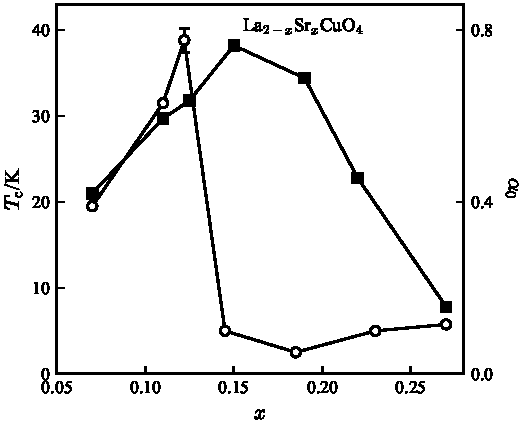
\includegraphics[width=7.5cm]{fig7-8.pdf}\\{\small 图 7.8\quad $\mathrm{La}_{2-x}\mathrm{Sr}_{x}\mathrm{CuO}_{4}$ 中 $T_{\mathrm{c}}$（■）和 $\alpha_{0}$（○）随 Sr 含量的变化关系}
\end{minipage}
\end{center}

在图7.9中，$\alpha_{\mathrm{Cu}}$ 也是从0.1（当 $x=0.15$ 时）迅速上升到0.8（当 $x=0.125$ 时）.此外，还可以清楚地看到，在La-214中无论是掺Ba或者是掺Sr，$\alpha_{0}$ 随x的变化落在同一条曲线上，考虑到 Sr 与 Ba 的质量相差颇大，但 $\alpha_{0}$ 的尖峰却都位于同一点（$x=1/8$ 处），我们完全有理由认为这一尖峰行为来源于电子效应，极有可能是和 $\mathrm{CuO}_{2}$ 电子态密度的尖峰（即近半满的二维布里渊区中电子态密度的范·霍夫奇性）有关.理论工作者在BCS声子机制范围内计入范·霍夫奇性对掺杂 La-214 系统的 $T_{\mathrm{c}}$ 和 $\alpha$ 的影响\textsuperscript{[24]}，解释了掺杂 La-214 中这一反常同位素效应，但却限于s波配对和电声子机制，不能全面地解释 La-214 铜氧化物的其它超导特征（如d波配对等）.换句话说，仅仅对同位素效应的反常作出解释仍不足以证实高温超导电性来源于电声子机制.

\begin{center}
\begin{minipage}{7.5cm}
\centering
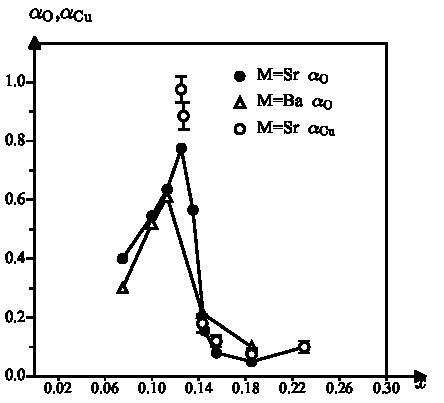
\includegraphics[width=7.5cm]{fig7-9.pdf}\\{\small 图 7.9\quad $\mathrm{La}_{2-x}\mathrm{M}_{x}\mathrm{CuO}_{4}$ 中的 $\alpha_{0}$、$\alpha_{\mathrm{Cu}}$ 随 x 变化曲线}
\end{minipage}
\end{center}

根据同位素效应的现有实验结果，人们既不能肯定，也不能否定高温超导电性来源于声子机制.尽管如此，在高温超导体中毕竟观察到了有限的 $\alpha$ 值，它至少暗示着在超导配对和凝聚的机制中包含有受声子效应影响的因素，有可能不是主要

的决定配对和凝聚的因素，但在解释同位素效应时却是不可忽略的.还应当指出，在La-214中观察到 $\alpha_{\mathrm{Cu}}$ 与 $\alpha_{0}$ 具有相同的数量级，表明当讨论电声子互作用对超导电性的影响时，$\mathrm{CuO}_{2}$ 平面上铜和氧离子的晶格振动是同等重要的.

最后，对常规和高温超导体中复杂的同位素效应作一个简单的小结.在常规的电声子机制BCS超导体中，尽管电性的库仑作用的影响曾使同位素效应变得十分复杂，但总趋势仍是以 $\alpha\approx1/2$ 的电声子机制为主导.目前，在高温超导体中的总趋势仍然是同位素效应普遍偏小，尽管在某些特殊情况下（如在弱掺杂区）声子效应不可忽略，使问题变得十分复杂，但是历史是值得借鉴的，作者仍相信配对的主要机制不是电声子互作用.

\subsection*{5. 不同于BCS超导体的低温特性}

除了 Nd-Ce-Cu-O 化合物以外，所有的铜氧化物高温超导体在 $T\ll T_{\mathrm{c}}$ 时均显示出与BCS超导体十分不同的特征.特别是超导态的低温电子比热容 $c_{\mathrm{s}}\left(T\ll T_{\mathrm{c}}\right)$、核自旋-点阵弛豫率 $T_{1\mathrm{s}}^{-1}\left(T\ll T_{\mathrm{c}}\right)$ 和伦敦穿透深度的变化 $\Delta\lambda(T)\equiv\lambda_{\mathrm{L}}(T)-\lambda_{\mathrm{L}}(0)$ 等物理量都表现为随温度变化的 $T^{n}$ 型简单幂次规律，而不是各向同性BCS超导体的 $\exp\left[-\Delta(0)/k_{\mathrm{B}}T\right]$ 型的指数激发特征.表7.4中列出了实验测量的结果，它们实际上是d波配对特征的反映.

表7.4\quad $T\ll T_{\mathrm{c}}$ 时高温超导体和BCS超导体的特性比较

\begin{center}\small
\begin{tabular}{lcc}
\hline
低温物性 & 高温超导体 & BCS超导体\\
\hline
$c_{\mathrm{s}}\left(T\ll T_{\mathrm{c}}\right)$ & $\sim T^{2}$ & $\sim\mathrm{e}^{-\Delta(0)/k_{\mathrm{B}}T}$\\
$\Delta\lambda\left(T\ll T_{\mathrm{c}}\right)$ & $\sim T$（$T^{2}$ 含杂） & $\sim\mathrm{e}^{-\Delta(0)/k_{\mathrm{B}}T}$\\
$T_{1\mathrm{s}}^{-1}\left(T\ll T_{\mathrm{c}}\right)$ & $\sim T^{3}$（$^{63}$Cu） & $\sim T\mathrm{e}^{-\Delta(0)/k_{\mathrm{B}}T}$\\
\hline
\end{tabular}
\end{center}

为了说明以上异常的低温特性，我们将先介绍各向异性超导电性，然后在§6中利用d波配对的超导理论作具体的解释.

\section{各向异性配对的超导电性}

上一章介绍的BCS超导理论是假定在费密面附近电子间的有效互作用矩阵元 $V\left(\boldsymbol{k},\boldsymbol{k}'\right)\approx-V$，即在能壳区内存在一个近似为常数的吸引势（$-V$）.这类吸引来源于电子间交换虚声子所形成的均匀净吸引互作用.按照此简化假定，求出的库柏对（也就是自旋单重态 $\left(\uparrow\downarrow-\downarrow\uparrow\right)/\sqrt{2}$ 配对）波函数和多体系统的能隙函数 $\Delta$ 均与电子间取向 $\left(\theta,\varphi\right)$ 无关，人们往往称之为各向同性超导体.近年来，大量实验事实已证明，还存在各向异性配对的超导体或超流体，其超导或超流序参量（即能隙函数）随取向 $\left(\theta,\varphi\right)$ 强烈变化，又称为各向异性配对超导（或超流）系统.在这类系统中，费密子间配对的自旋态既可能是单重态：$\left(\uparrow\downarrow-\downarrow\uparrow\right)/\sqrt{2}$，也可能是三重态：$\uparrow\uparrow$、$\downarrow\downarrow$ 及 $\left(\uparrow\downarrow+\downarrow\uparrow\right)/\sqrt{2}$.这时导致配对的主要相互作用不再是来源于交换虚声子，而是由于费密子间的强烈同位（即同一格点上的）库仑排斥作用（又称强关联）所激发的其它类型的波色子传递而形成的有效互作用.例如，在超流 $^{3}\mathrm{He}$ 系统中所形成的核自旋三重态各向异性配对来源于 $^{3}\mathrm{He}$ 原子间交换铁磁性自旋涨落，而在重费密子系统及氧化氧高温超导体中的发现的自旋单重态各向异性d波配对超导电性，尽管其微观机理至今尚未确定，但是强同位库仑关联所激发的反铁磁自旋涨落至少可认为是有利于形成各向异性d波配对的一种可能机制.

为了研究各向异性配对超导或超流，有必要将BCS理论推广用于任意有效互作用和任意自旋取向配对情形.为使物理图像明确，先讨论单个对（即广义的库柏对）问题，然后再推广到多体系统求能隙函数.

\subsection*{1. 广义库柏对}

现在将第六章§3中所讨论的一对自旋取向反平行电子之间配对的库柏问题推广到包括自旋平行与反平行配对的一般情形.类似于习题(27)，在这里仍讨论在填满的费密球之外存在两个相互作用的费密子的量子力学问题.不同之处在于它们是具有任意自旋取向的两个费密子 $\left(\boldsymbol{r}_{1},\sigma_{1}\right)$ 与 $\left(\boldsymbol{r}_{2},\sigma_{2}\right)$，其间仅在费密面外 $\hbar\omega_{0}$ 宽度的能壳区内存在有效互作用 $V\left(\left|\boldsymbol{r}_{1}-\boldsymbol{r}_{2}\right|\right)$，这时两费密子系统的波函数 $\psi\left(\boldsymbol{r}_{1}\sigma_{1};\boldsymbol{r}_{2}\sigma_{2}\right)$ 满足定态薛定谔方程
\begin{equation}
  \left\{-\left(\hbar^{2}/2m\right)\left(\nabla_{1}^{2}+\nabla_{2}^{2}\right)
  +V\left(\left|\boldsymbol{r}_{1}-\boldsymbol{r}_{2}\right|\right)-E'\right\}
  \psi\left(\boldsymbol{r}_{1}\sigma_{1};\boldsymbol{r}_{2}\sigma_{2}\right)=0
\end{equation}
在质心动量等于零时，是一对动量相反的费密子（即取 $\boldsymbol{k}_{1}+\boldsymbol{k}_{2}=\boldsymbol{0}$），这时二体波函数可简单地写为
\begin{equation}
  \psi\left(\boldsymbol{r}_{1}\sigma_{1};\boldsymbol{r}_{2}\sigma_{2}\right)
  =\varphi\left(\boldsymbol{r}_{1}-\boldsymbol{r}_{2}\right)\chi\left(\sigma_{1},\sigma_{2}\right)
\end{equation}
其中空间部分只是相对坐标 $\boldsymbol{r}=\boldsymbol{r}_{1}-\boldsymbol{r}_{2}$ 的函数.由于 $\psi$ 应具有全同费密子系统的反对称特征，当自旋波函数 $\chi\left(\sigma_{1},\sigma_{2}\right)$ 为单重态时，其轨道部分 $\varphi\left(\boldsymbol{r}_{1}-\boldsymbol{r}_{2}\right)$ 必须为 $\boldsymbol{r}_{1}-\boldsymbol{r}_{2}$ 的偶函数，这是偶宇称情形，而当 $\chi\left(\sigma_{1},\sigma_{2}\right)$ 为自旋三重态时，则要求 $\varphi\left(\boldsymbol{r}_{1}-\boldsymbol{r}_{2}\right)$ 为奇函数，属于奇宇称情形.

由于有效势V与自旋无关，式(7.4.1)在相对坐标（$\boldsymbol{r}\equiv\boldsymbol{r}_{1}-\boldsymbol{r}_{2}$）中可用 $\varphi(\boldsymbol{r})$ 表示
\begin{equation}
  \left[-\left(\hbar^{2}/m\right)\nabla^{2}+V(\boldsymbol{r})\right]\varphi(\boldsymbol{r})=E'\varphi(\boldsymbol{r})
\end{equation}
其中 $\varphi(\boldsymbol{r})$ 代表相对运动的轨道波函数.对 $\varphi(\boldsymbol{r})$ 作傅里叶变换
\begin{equation}
  \varphi(\boldsymbol{r})=\sum_{\boldsymbol{k}}\varphi(\boldsymbol{k})\,\mathrm{e}^{\mathrm{i}\boldsymbol{k}\cdot\boldsymbol{r}}
\end{equation}
并写出有效互作用的矩阵元
\begin{equation}
  V\left(\boldsymbol{k},\boldsymbol{k}'\right)=\int\mathrm{d}^{3}r\,
  \mathrm{e}^{-\mathrm{i}\left(\boldsymbol{k}-\boldsymbol{k}'\right)\cdot\boldsymbol{r}}V(\boldsymbol{r})
\end{equation}
则式(7.4.3)变为
\begin{equation}
  \left(2E_{k}-E'\right)\varphi(\boldsymbol{k})=-\sum_{\boldsymbol{k}'}V\left(\boldsymbol{k},\boldsymbol{k}'\right)\varphi(\boldsymbol{k}')
  \qquad\left[E_{k}\equiv\left(\hbar^{2}k^{2}/2m\right)\right]
\end{equation}
取费密能 $E_{\mathrm{F}}=\left(\hbar^{2}k_{\mathrm{F}}^{2}/2m\right)$ 作为能量的原点，并定义
\begin{equation}
  \varepsilon_{k}\equiv E_{k}-E_{\mathrm{F}}\ ,\quad E\equiv E'-2E_{\mathrm{F}}
\end{equation}
可将式(7.4.6)改写为
\begin{equation}
  \left(2\varepsilon_{k}-E\right)\varphi(\boldsymbol{k})=-\sum_{\boldsymbol{k}'}V\left(\boldsymbol{k},\boldsymbol{k}'\right)\varphi(\boldsymbol{k}')
\end{equation}
当基体材料为各向同性时，$V\left(\boldsymbol{k},\boldsymbol{k}'\right)$ 只是 $\left|\boldsymbol{k}-\boldsymbol{k}'\right|=k^{2}+k'^{2}-2kk'\cos\theta_{\boldsymbol{k}\boldsymbol{k}'}$ 的函数，并且由于V仅在费密面附近不为零，可近似取 $k=k'=k_{\mathrm{F}}$，这时 $V\left(\boldsymbol{k},\boldsymbol{k}'\right)$ 只是 k 与 $\boldsymbol{k}'$ 费密子间夹角余弦 $\cos\theta_{\boldsymbol{k}\boldsymbol{k}'}$ 的函数.按此，V可用勒让德函数展开
\begin{equation}
  V\left(\boldsymbol{k},\boldsymbol{k}'\right)=V\left(\hat{\boldsymbol{k}}\cdot\hat{\boldsymbol{k}}'\right)
  =V\left(\cos\theta_{\boldsymbol{k}\boldsymbol{k}'}\right)
  =\sum_{l}\left(2l+1\right)V_{l}\,\mathrm{P}_{l}\left(\cos\theta_{ll'}\right)
\end{equation}
其中 $\hat{\boldsymbol{k}}$ 为k方向的单位矢，而l分波势
\begin{equation}
\begin{aligned}
  V_{l}&=\frac{1}{2}\int_{-1}^{1}\mathrm{d}\left(\cos\theta_{\boldsymbol{k}\boldsymbol{k}'}\right)
  V\left(\cos\theta_{\boldsymbol{k}\boldsymbol{k}'}\right)\mathrm{P}_{l}\left(\cos\theta_{\boldsymbol{k}\boldsymbol{k}'}\right)\\
  &=\int_{\mathrm{FS}}\frac{\mathrm{d}\Omega}{4\pi}\,V\left(\boldsymbol{k},\boldsymbol{k}'\right)\mathrm{P}_{l}\left(\cos\theta_{\boldsymbol{k}\boldsymbol{k}'}\right)
\end{aligned}
\end{equation}
显然 $V_{l}$ 是一个只与 $k_{\mathrm{F}}$ 有关的常数，它仅在费密球外 $0\leqslant\varepsilon_{k}\leqslant\hbar\omega_{0}$ 能壳内不为零.利用数学等式
\begin{equation}
  \mathrm{P}_{l}\left(\cos\theta_{\boldsymbol{k}\boldsymbol{k}'}\right)=\frac{4\pi}{\left(2l+1\right)}
  \sum_{m=-l}^{l}\mathrm{Y}_{lm}\left(\theta_{\boldsymbol{k}},\phi_{\boldsymbol{k}}\right)
  \mathrm{Y}_{lm}^{*}\left(\theta_{\boldsymbol{k}'},\phi_{\boldsymbol{k}'}\right)
\end{equation}
其中 $\left(\theta_{\boldsymbol{k}},\phi_{\boldsymbol{k}}\right)$ 与 $\left(\theta_{\boldsymbol{k}'},\phi_{\boldsymbol{k}'}\right)$ 分别代表 k 与 $\boldsymbol{k}'$ 的方位角，将式(7.4.9)与式(7.4.11)代入式(7.4.8)，并利用谐球函数 $\mathrm{Y}_{lm}$ 的正交归一性
\begin{equation}
\begin{aligned}
  \delta_{ll'}\delta_{mm'}&=\int\mathrm{d}\Omega\,\mathrm{Y}_{lm}^{*}\left(\theta_{\boldsymbol{k}},\phi_{\boldsymbol{k}}\right)
  \mathrm{Y}_{l'm'}\left(\theta_{\boldsymbol{k}},\phi_{\boldsymbol{k}}\right)\\
  &=\int_{0}^{\pi}\mathrm{d}\theta_{\boldsymbol{k}}\int_{0}^{2\pi}\mathrm{d}\phi_{\boldsymbol{k}}\,
  \mathrm{Y}_{lm}^{*}\left(\theta_{\boldsymbol{k}},\phi_{\boldsymbol{k}}\right)
  \mathrm{Y}_{l'm'}\left(\theta_{\boldsymbol{k}},\phi_{\boldsymbol{k}}\right)
\end{aligned}
\end{equation}
容易证明，对于确定的l与m，式(7.4.8)的本征函数 $\varphi(\boldsymbol{k})$ 可简单取下列特解：
\begin{subequations}
\begin{equation}
  \varphi(\boldsymbol{k})=\psi_{l}(\boldsymbol{k})\,\mathrm{Y}_{lm}\left(\theta_{\boldsymbol{k}},\phi_{\boldsymbol{k}}\right)
\end{equation}
其中l分波的振幅 $\psi_{l}(\boldsymbol{k})$（$k=\left|\boldsymbol{k}\right|$ 与方位无关）满足方程
\begin{equation}
\begin{aligned}
  \left(2\varepsilon_{k}-E\right)\psi_{l}(k)
  &=-\frac{V_{l}}{\left(2\pi\right)^{3}}\int_{\varepsilon_{k'}=0}^{\varepsilon_{k'}=\hbar\omega_{0}}
  4\pi k'^{2}\psi_{l}(k')\,\mathrm{d}k'\\
  &=-V_{l}\sum_{k>k_{\mathrm{F}}}\psi_{l}(k')
  \qquad\left(0\leqslant\varepsilon_{k'}\leqslant\hbar\omega_{0}\right)
\end{aligned}
\end{equation}
\end{subequations}
令 $\sum\limits_{k'>k_{\mathrm{F}}}\psi_{l}(k')\equiv A$，代入式(7.4.13b)，得到 $\psi_{l}(k)=-V_{l}A/\left(2\varepsilon_{k}-E\right)$，再对k求和，可求出对于A的非零解应满足下列自洽方程：
\begin{equation}
  1=-V_{l}\sum_{k>k_{\mathrm{F}}}\frac{1}{2\varepsilon_{k}-E}
  \qquad\left(0\leqslant\varepsilon_{k}\leqslant\hbar\omega_{0}\right)
\end{equation}
考虑到 $\hbar\omega_{0}\ll E_{\mathrm{F}}$，上式可近似为
\begin{equation}
  1=-g(0)V_{l}\int_{0}^{\hbar\omega_{0}}\frac{\mathrm{d}\varepsilon}{2\varepsilon-E}
  =-g(0)V_{l}\ln\left(\frac{2\hbar\omega_{0}-E}{-E}\right)
\end{equation}
显然，当 $V_{l}<0$ 时，求出的能量 $E<0$，这时E代表l分波配对态的能量
\begin{equation}
  E=-\frac{2\hbar\omega_{0}}{\exp\left[2/g(0)\left|V_{l}\right|\right]-1}
\end{equation}
即使当吸引互作用很弱且满足 $g(0)\left|V_{l}\right|\ll1$ 时，也可得到类似(6.3.11)的束缚对态
\begin{equation}
  E=-2\hbar\omega_{0}\exp\left[-2/g(0)\left|V_{l}\right|\right]<0
\end{equation}
说明形成了l分波的束缚对.以上讨论表明：通常只需在 $V\left(\boldsymbol{k},\boldsymbol{k}'\right)$ 的分波展开式(7.4.9)中取最大 $\left|V_{l}\right|$ 的吸引项，即可构成l分波配对的束缚态 $E<0$，它反而比费密球内侧无相互作用的电子对能量还要低，这自然将使费密球内侧的电子自动溢出，从而导致费密球态失稳，这是形成l波配对超导的信号.由于l分波的k空间波函数为 $\varphi(\boldsymbol{k})=\psi_{l}(k)\mathrm{Y}_{lm}\left(\theta_{\boldsymbol{k}},\phi_{\boldsymbol{k}}\right)$，显然只要 $l>0$，$\varphi(\boldsymbol{k})$ 就是随方位 $\theta_{\boldsymbol{k}}$ 与 $\phi_{\boldsymbol{k}}$ 变化的各向异性函数，因此 $l>0$ 分波配对又可称为各向异性配对.

现在进一步讨论配对态轨道部分的宇称与 $\varphi(\boldsymbol{k})$ 的关系.前文中已指出，当配对费密子的自旋处于单重态时，$\varphi\left(\boldsymbol{r}=\boldsymbol{r}_{1}-\boldsymbol{r}_{2}\right)$ 为偶函数，其傅里叶变换也应为k的偶函数，这时轨道部分只能取 $\mathrm{Y}_{lm}$ 中 $l=0,\ 2,\ \cdots$ 诸偶数.反之，配对费密子的自旋取三重态时，由于要求轨道部分 $\varphi\left(\boldsymbol{r}\right)$ 为r的奇函数，则 $\varphi(\boldsymbol{k})$ 就只能取 $\mathrm{Y}_{lm}$ 中 $l=1,\ 3,\ 5,\ \cdots$ 诸奇数，构成k的奇函数.以上讨论可归结为

表7.5

\begin{center}\small
\begin{tabular}{lcc}
\hline
 & 自旋单重态 & 自旋三重态\\
\hline
自旋波函数 $\chi\left(\sigma_{1},\sigma_{2}\right)$ &
$\left(\uparrow\downarrow-\downarrow\uparrow\right)/\sqrt{2}$ &
$\uparrow\uparrow$，$\downarrow\downarrow$，$\left(\uparrow\downarrow+\downarrow\uparrow\right)/\sqrt{2}$\\
轨道波函数 $\mathrm{Y}_{lm}\left(\theta_{\boldsymbol{k}},\phi_{\boldsymbol{k}}\right)$ &
$l=$ 偶数 $\left(0,2,4,\cdots\right)$ & $l=$ 奇数 $\left(1,3,5,\cdots\right)$\\
 & s波 $\left(l=0\right)$，d波 $\left(l=2\right)$ & p波 $\left(l=1\right)$\\
\hline
轨道宇称 & 偶 & 奇\\
\hline
\end{tabular}
\end{center}

由此可知，除了 $l=0$ 的s波配对是各向同性配对以外，所有的 $l>0$ 分波，其 $\varphi(\boldsymbol{k})$ 均按 $\mathrm{Y}_{lm}\left(\theta_{\boldsymbol{k}},\phi_{\boldsymbol{k}}\right)$ 随k的方位变化.推广到多个对情形，其能隙函数也应当是随方位 $\hat{\boldsymbol{k}}$（$\hat{\boldsymbol{k}}\equiv\boldsymbol{k}/\left|\boldsymbol{k}\right|$）变化的函数，这就是各向异性超导体的特征.

在实际计算时，应具体给出有效势 $V(\boldsymbol{r})$ 及其矩阵元 $V\left(\boldsymbol{k},\boldsymbol{k}'\right)$.在 $^{3}\mathrm{He}$ 液体中，实验已证实超流来源于两个 $^{3}\mathrm{He}$ 原子核自旋的三重态配对，其轨道部分为 $l=1$ 的p波配对.理论上，人们计算出在 $^{3}\mathrm{He}$ 原子间交换铁磁（FM）自旋涨落时，有效势的诸分量中 $V_{l=1}<0$，且其数值 $\left|V_{1}\right|$ 为最大，这将导致轨道部分形成奇宇称的p波配对.在高温超导体中，实验已证实轨道部分主要是d波偶宇称配对.理论上人们用强关联模型解释，因为强关联体系的特征是存在很强的同位库仑排斥作用，它将阻止s波配对的形成，由于s轨道的径向波函数在r较小时仍然很大，同位库仑关联对s波配对的影响将是十分显著的.但是强关联的理论却允许形成d波配对，因为在量子力学中已知，d轨道的径向波函数在r很小时存在零点，因此即使在强关联存在时，同位库仑排斥作用也不会对d波产生显著的影响，这就是在铜氧化物强关联体系中有利于形成d波配对的原因.至于重费密子体系，尽管实验尚无定论，但多数研究者认为配对的吸引作用来源于重费密子间交换反铁磁（AFM）自旋涨落，并已证明在这种有效互作用势中 $V_{l=2}$ 为最大吸引分波势，从而预言重费密子超导体中也是以d波配对为主导的各向异性超导体.

\subsection*{2. 各向异性能隙函数}

现在将上述理论推广到多体系统，求解各向异性超导体的能隙函数.为简单起见，我们仅限于讨论自旋反平行电子间的单重态配对，因为实验已证明氧化物高温超导体中仍是 $\uparrow$，$\downarrow$ 自旋电子间配对所形成的各向异性超导体.设形成超导的有效互作用为
\begin{equation}
  H_{\mathrm{eff}}=\sum_{k,k'}V\left(\boldsymbol{k},\boldsymbol{k}'\right)C^{+}_{k'}C^{+}_{-k'}C_{-k}C_{k}
\end{equation}
其中仍系采用简化记号 $k\equiv\left(\boldsymbol{k},\uparrow\right)$，$-k\equiv\left(-\boldsymbol{k},\downarrow\right)$.有效互作用矩阵元 $V\left(\boldsymbol{k},\boldsymbol{k}'\right)$ 仍由式(7.4.5)描述，它只是 k 与 $\boldsymbol{k}'$ 间夹角余弦的函数，可根据式(7.4.9)作分波展开，并且仅在费密面附近能壳区 $-\hbar\omega_{0}\leqslant\varepsilon_{k},\varepsilon_{k}\leqslant\hbar\omega_{0}$ 内不为零.式(7.4.18)与BCS有效互作用式(6.2.8)之差别在于，现在的 $V\left(\boldsymbol{k},\boldsymbol{k}'\right)=V\left(\hat{\boldsymbol{k}}\cdot\hat{\boldsymbol{k}}'\right)$ 是各向异性的，而不再取BCS的各向同性s波分波势假定 $V\left(\boldsymbol{k},\boldsymbol{k}'\right)=-V$.

当存在自旋单重态配对时，费密面附近一对动量与自旋取向均相反的电子间将形成 $\left(\boldsymbol{k}\uparrow,-\boldsymbol{k}\downarrow\right)$ 型库柏对，使对算符的下列平均不为零
\begin{equation}
  \langle C_{-k}C_{k}\rangle_{T}\neq0\,,\qquad
  \langle C^{+}_{k}C^{+}_{-k}\rangle_{T}\neq0
\end{equation}
在自洽场近似下，与式(6.4.4)对应的约化哈密顿量为
\begin{equation}
\begin{aligned}
  \overline{H}&=\sum_{k}\varepsilon_{k}\left(C^{+}_{k}C_{k}+C^{+}_{-k}C_{-k}\right)
  +\sum_{k,k'}V\left(\boldsymbol{k},\boldsymbol{k}'\right)\left\{C^{+}_{k}C^{+}_{-k}\langle C_{-k'}C_{k'}\rangle_{T}\right.\\
  &\quad\left.+C_{-k}C_{k}\langle C^{+}_{k'}C^{+}_{-k'}\rangle_{T}\right\}
  -\sum_{k,k'}V\left(\boldsymbol{k},\boldsymbol{k}'\right)
  \langle C^{+}_{k'}C^{+}_{-k'}\rangle_{T}\langle C_{-k}C_{k}\rangle_{T}
\end{aligned}
\end{equation}
类似于式(6.4.5)，定义各向异性的能隙函数
\begin{equation}
  \Delta(\boldsymbol{k})=-\sum_{k'}V\left(\boldsymbol{k},\boldsymbol{k}'\right)
  \langle C_{-k'}C_{k'}\rangle_{T}
\end{equation}
并将 $\overline{H}$ 用 $\Delta(\boldsymbol{k})$ 表示为
\begin{equation}
  \overline{H}=\sum_{k}\varepsilon_{k}\left(C^{+}_{k}C_{k}+C^{+}_{-k}C_{-k}\right)
  -\sum_{k}\left\{\Delta(\boldsymbol{k})C^{+}_{k}C^{+}_{-k}
  +\Delta^{*}(\boldsymbol{k})C_{-k}C_{k}\right\}
  +\sum_{k}\Delta(\boldsymbol{k})\langle C^{+}_{k}C^{+}_{-k}\rangle_{T}
\end{equation}
上式既可用 $u$-$v$ 变换方法，也可用格林函数方法求解.我们将采用附录C中介绍的格林函数运动方程方法直接求出 $T>0$ 时的元激发和能隙函数 $\Delta(\boldsymbol{k})$.根据格林函数运动方程的通式
\begin{equation*}
  \omega\ll A\mid B\gg_{\omega}=\langle[A,B]_{+}\rangle
  +\ll[A,\overline{H}]_{-}\gg\mid B\gg_{\omega}\tag{C.7}
\end{equation*}
取 $A=C_{k}$ 及 $B=C_{-k}$，得到
\begin{subequations}
\begin{equation}
  \left(\omega-\varepsilon_{k}\right)\ll C_{k}\mid C_{-k}\gg_{\omega}
  =-\Delta(\boldsymbol{k})\ll C^{+}_{-k}\mid C_{-k}\gg_{\omega}
\end{equation}
再取 $A=C^{+}_{-k}$ 及 $B=C_{-k}$，又得
\begin{equation}
  \left(\omega+\varepsilon_{k}\right)\ll C^{+}_{-k}\mid C_{-k}\gg_{\omega}
  =-\Delta^{*}(\boldsymbol{k})\ll C_{k}\mid C_{-k}\gg_{\omega}
\end{equation}
\end{subequations}
到此方程组已封闭，经简单运算可求出
\begin{equation}
\begin{aligned}
  \ll C_{k}\mid C_{-k}\gg_{\omega}
  &=\frac{-\Delta(\boldsymbol{k})}{\left[\omega^{2}-\left(\varepsilon_{k}^{2}+\Delta(\boldsymbol{k})\Delta^{*}(\boldsymbol{k})\right)\right]}\\
  &=\left[\frac{\Delta(\boldsymbol{k})}{2\hat{\xi}_{k}}\right]
  \left[\frac{1}{\omega+\hat{\xi}_{k}}-\frac{1}{\omega-\hat{\xi}_{k}}\right]
\end{aligned}
\end{equation}
其中格林函数的极点为
\begin{equation}
  \hat{\xi}_{k}=\sqrt{\varepsilon_{k}^{2}+\left|\Delta(\boldsymbol{k})\right|^{2}}
\end{equation}
代表各向异性超导体中的元激发.读者不难自行验证，$\omega=\hat{\xi}_{k}$ 不仅是 $\ll C_{k}\mid C_{-k}\gg_{\omega}$ 的极点，也是 $\ll C^{+}_{-k}\mid C_{-k}\gg_{\omega}$ 与 $\ll C_{k}\mid C^{+}_{k}\gg_{\omega}$ 等的共同极点.因此，$\hat{\xi}_{k}$ 确实代表超导体中的元激发.

由于推迟格林函数 $\ll C_{k}\mid C_{-k}\gg_{\omega+\mathrm{i}\eta}$ 的虚部为
\begin{equation}
  -\left(\frac{1}{\pi}\right)\mathrm{Im}\ll C_{k}\mid C_{-k}\gg_{\omega+\mathrm{i}\eta}
  =\left[\frac{\Delta(\boldsymbol{k})}{2\hat{\xi}_{k}}\right]
  \left\{\delta\left(\omega+\hat{\xi}_{k}\right)-\delta\left(\omega-\hat{\xi}_{k}\right)\right\}
\end{equation}
利用格林函数的谱定理式(A.28)，可求出
\begin{equation}
  \langle C_{-k}C_{k}\rangle_{T}
  =\int_{-\infty}^{\infty}\mathrm{d}\omega\,
  \frac{\left\{-\dfrac{1}{\pi}\mathrm{Im}\ll C_{k}\mid C_{-k}\gg_{\omega+\mathrm{i}\eta}\right\}}{\mathrm{e}^{\beta\omega}+1}
  =\frac{\Delta(\boldsymbol{k})}{2\hat{\xi}_{k}}\tanh\left(\frac{1}{2}\beta\hat{\xi}_{k}\right)
\end{equation}
其中 $\beta=\left(k_{\mathrm{B}}T\right)^{-1}$.将上式代入能隙的定义式(7.4.21)，得到一个随 $\hat{\boldsymbol{k}}$ 取向变化的自洽方程
\begin{equation}
  \Delta\left(\hat{\boldsymbol{k}},T\right)=-\frac{1}{2}\sum_{k'}V\left(\hat{\boldsymbol{k}}\cdot\hat{\boldsymbol{k}}'\right)
  \Delta\left(\hat{\boldsymbol{k}}',T\right)
  \frac{\tanh\left(\dfrac{1}{2}\beta\hat{\xi}_{k'}\right)}{\hat{\xi}_{k'}}
\end{equation}
其中 $\hat{\xi}_{k}=\sqrt{\hat{\epsilon}_{k}^{2}+\left|\Delta(\hat{\boldsymbol{k}},T)\right|^{2}}$ 也是随 $\hat{\boldsymbol{k}}$ 取向变化的.由于 $V\left(\hat{\boldsymbol{k}},\hat{\boldsymbol{k}}'\right)$ 可按照式(7.4.9)作分波展开，当略去不同l分波间的耦合时，可以仅取式(7.4.9)中的一个具有最大吸引作用的分波项 $-\left(2l+1\right)\allowbreak\left|V_{l}\right|\allowbreak\mathrm{P}_{l}\left(\hat{\boldsymbol{k}}\cdot\hat{\boldsymbol{k}}'\right)$，这时存在 $\Delta\left(\hat{\boldsymbol{k}},T\right)\sim\mathrm{Y}_{lm}\left(\theta_{\boldsymbol{k}},\phi_{\boldsymbol{k}}\right)$ 的简单解
\begin{equation}
  \Delta\left(\hat{\boldsymbol{k}},T\right)=\Delta_{\mathrm{a}}(T)\sqrt{4\pi}\,\mathrm{Y}_{lm}\left(\theta_{\boldsymbol{k}},\phi_{\boldsymbol{k}}\right)
\end{equation}
其中取 $\sqrt{4\pi}$ 因子是为了保证取向平均：$\int\left(\mathrm{d}\Omega_{k}/4\pi\right)\left|\Delta(\hat{\boldsymbol{k}},T)\right|^{2}=\Delta_{\mathrm{a}}^{2}(T)$，在这里 $\Delta_{\mathrm{a}}(T)$ 称为能隙在费密面上的取向平均值.将此简解式(7.4.29)代入式(7.4.28)，并利用 $\mathrm{Y}_{lm}$ 的正交归一条件式(7.4.12)和球函数的展式(7.4.9)—(7.4.11)，可求出这个简单解所满足的自洽方程
\begin{subequations}
\begin{equation}
  1=\frac{1}{2}\left|V_{l}\right|\sum_{k'}
  \frac{4\pi\left|\mathrm{Y}_{lm}(\hat{\boldsymbol{k}}')\right|^{2}\tanh\left(\dfrac{1}{2}\beta\hat{\xi}_{k'}\right)}{\hat{\xi}_{k'}}
\end{equation}
其中
\begin{equation}
  \hat{\xi}_{k'}=\sqrt{\varepsilon_{k'}^{2}+4\pi\Delta_{\mathrm{a}}^{2}(T)\left|\mathrm{Y}_{lm}(\hat{\boldsymbol{k}}')\right|^{2}}
\end{equation}
\end{subequations}
尽管式(7.4.28)是从自旋单重态配对导出的，对于自旋三重态配对所求得的自洽方程也是相同.它们的差别仅在于对自旋的单重态l取偶数，而对于自旋三重态配对l取奇数.因此，式(7.4.28)—(7.4.30)是适用于p波与d波配对的普遍公式.作为这类简单解一个典型例子是 $^{3}\mathrm{He}$ 中的超流A相，它是p波 $\left(l=1\right)$ 的等自旋（ESP）态 $m=\pm1$.因此，等自旋态的能隙函数 $\Delta_{\mathrm{A}}\left(\hat{\boldsymbol{k}},T\right)$ 的模平方可表示为
\begin{equation}
  \left|\Delta_{\mathrm{A}}\left(\hat{\boldsymbol{k}},T\right)\right|^{2}
  =\Delta_{\mathrm{a}}^{2}(T)\left|\sqrt{4\pi}\,\mathrm{Y}_{l=1,m=\pm1}(\hat{\boldsymbol{k}})\right|^{2}
  =\frac{3}{2}\Delta_{\mathrm{a}}^{2}(T)\sin^{2}\theta_{\boldsymbol{k}}
\end{equation}
将上式代入式(7.4.30)，得到p波等自旋态的能隙方程
\begin{subequations}
\begin{equation}
  1=\frac{1}{2}\left|V_{1}\right|\sum_{k'}4\pi\left|\mathrm{Y}_{l=1,m=\pm1}(\hat{\boldsymbol{k}}')\right|^{2}
  \frac{\tanh\left(\dfrac{1}{2}\beta\hat{\xi}_{k'}\right)}{\hat{\xi}_{k'}}
\end{equation}
其中
\begin{equation}
  \hat{\xi}_{k'}=\sqrt{\varepsilon_{k'}^{2}+\left|\Delta_{\mathrm{A}}\left(\hat{\boldsymbol{k}}',T\right)\right|^{2}}
\end{equation}
\end{subequations}
当 $T=T_{\mathrm{c}}$ 时，由于 $\Delta_{\mathrm{A}}\left(\hat{\boldsymbol{k}},T_{\mathrm{c}}\right)=0$，上式中 $\hat{\xi}_{k'}$ 简化为 $\left|\varepsilon_{k'}\right|$.经角积分后，求得其 $T_{\mathrm{c}}$ 方程为
\begin{subequations}
\begin{equation}
  1=g(0)\left|V_{1}\right|\int_{0}^{\hbar\omega_{0}}
  \frac{\tanh\left(\dfrac{1}{2}\beta_{\mathrm{c}}\varepsilon\right)}{\varepsilon}\,\mathrm{d}\varepsilon
\end{equation}
其中 $\beta_{\mathrm{c}}=\left(k_{\mathrm{B}}T_{\mathrm{c}}\right)^{-1}$，从而求出与式(6.5.10)相似的p波超流相的转变温度
\begin{equation}
  k_{\mathrm{B}}T_{\mathrm{c}}=\frac{2\mathrm{e}^{\gamma}}{\pi}\hbar\omega_{0}
  \exp\left[\frac{-1}{g(0)\left|V_{1}\right|}\right]
  \approx1.13\,\hbar\omega_{0}\exp\left[\frac{-1}{g(0)\left|V_{1}\right|}\right]
\end{equation}
\end{subequations}
若将上式中 $\left|V_{1}\right|$ 换成 $\left|V_{l}\right|$，它就是l波超导（或超流）态的转变温度，与从式(7.4.30)求出的l分波 $T_{\mathrm{c}}$ 公式一致.换句话说，各向异性超导（或超流）体的 $T_{\mathrm{c}}$ 公式具有与BCS超导体相同的形式.

p波等自旋态的零温能隙公式也可从式(7.4.32)求得，它满足
\begin{subequations}
\begin{equation}
\begin{aligned}
  1&=\frac{1}{2}\left|V_{1}\right|\sum_{k'}
  \frac{4\pi\left|\mathrm{Y}_{l=1,m=\pm1}(\hat{\boldsymbol{k}}')\right|^{2}}
  {\sqrt{\varepsilon_{k'}^{2}+\left|\Delta_{\mathrm{A}}(\hat{\boldsymbol{k}}',0)\right|^{2}}}\\
  &=g(0)\left|V_{1}\right|\int\mathrm{d}\Omega_{k'}\,
  \left|\mathrm{Y}_{l=1,m=\pm1}\left(\theta_{\boldsymbol{k}'},\phi_{\boldsymbol{k}'}\right)\right|^{2}\times\\
  &\quad\int_{0}^{\hbar\omega_{0}}\frac{\mathrm{d}\varepsilon'}
  {\sqrt{\varepsilon'^{2}+\dfrac{3}{2}\Delta_{\mathrm{a}}^{2}(0)\sin^{2}\theta_{\boldsymbol{k}'}}}\\
  &=g(0)\left|V_{1}\right|\cdot\frac{3}{4}\int_{-1}^{+1}\mathrm{d}\cos\theta_{\boldsymbol{k}'}
  \left(1-\cos^{2}\theta_{\boldsymbol{k}'}\right)\times\\
  &\quad\ln\left[\frac{2\hbar\omega_{0}}{\sqrt{\dfrac{3}{2}}\,\Delta_{\mathrm{a}}(0)\left|\sin\theta_{\boldsymbol{k}'}\right|}\right]
\end{aligned}
\end{equation}
在最后一个等式中应用了弱耦合BCS理论的近似条件 $\hbar\omega_{0}\gg\left|\Delta_{\mathrm{A}}(\hat{\boldsymbol{k}},0)\right|$.设 $x=\cos\theta_{\boldsymbol{k}}$，再将上式对数项中含x部分分离为
\begin{equation*}
  \ln\left[\frac{2\hbar\omega_{0}}{\sqrt{\dfrac{3}{2}}\,\Delta_{\mathrm{a}}(0)\sqrt{1-x^{2}}}\right]
  =\ln\left[\frac{2\hbar\omega_{0}}{\sqrt{\dfrac{3}{2}}\,\Delta_{\mathrm{a}}(0)}\right]
  -\frac{1}{2}\ln\left(1-x^{2}\right)
\end{equation*}
并利用积分公式
\begin{equation*}
\begin{aligned}
  &\frac{3}{4}\int_{-1}^{1}\mathrm{d}x\,\left(1-x^{2}\right)=1\\
  &\frac{3}{4}\int_{-1}^{1}\mathrm{d}x\,\left(1-x^{2}\right)\cdot\frac{1}{2}\ln\left(1-x^{2}\right)=\ln 2-\frac{5}{6}
\end{aligned}
\end{equation*}
可算出式(7.4.34)中的所有积分，得到等式
\begin{equation}
\begin{aligned}
  1&=g(0)\left|V_{1}\right|\left\{\ln\left[\frac{2\hbar\omega_{0}}{\Delta_{\mathrm{a}}(0)}\right]
  -\left[\ln\sqrt{6}-\frac{5}{6}\right]\right\}\\
  &=g(0)\left|V_{1}\right|\ln\left\{\left[\frac{2\hbar\omega_{0}}{\Delta_{\mathrm{a}}(0)}\right]\cdot\left[\frac{\mathrm{e}^{5/6}}{\sqrt{6}}\right]\right\}
\end{aligned}
\end{equation}
\end{subequations}
最后求出等自旋态的零温平均能隙值
\begin{equation}
\begin{aligned}
  \Delta_{\mathrm{a}}^{\mathrm{ESP}}(0)
  &=\frac{\mathrm{e}^{5/6}}{\sqrt{6}}\cdot2\hbar\omega_{0}
  \exp\left[\frac{-1}{g(0)\left|V_{1}\right|}\right]\\
  &=0.94\cdot2\hbar\omega_{0}\exp\left[\frac{-1}{g(0)\left|V_{1}\right|}\right]
\end{aligned}
\end{equation}
它略小于BCS值 $2\hbar\omega_{0}\exp\left[-1/g(0)\left|V_{1}\right|\right]$.因此，在各向异性配对超流体的等自旋态中，零温平均能隙与转变温度 $T_{\mathrm{c}}$ 的比值仍然是一个与材料特性无关的常数，但其比值却小于BCS的普适常数3.53.
\begin{equation}
\begin{aligned}
  \left[\frac{2\Delta_{\mathrm{a}}(0)}{k_{\mathrm{B}}T_{\mathrm{c}}}\right]^{\mathrm{ESP}}
  &=(0.94)\cdot\left(2\pi\mathrm{e}^{-\gamma}\right)\\
  &=(0.94)\left[\frac{2\Delta_{\mathrm{a}}(0)}{k_{\mathrm{B}}T_{\mathrm{c}}}\right]^{\mathrm{BCS}}<3.53
\end{aligned}
\end{equation}
比值 $\left[\dfrac{2\Delta_{\mathrm{a}}(0)}{k_{\mathrm{B}}T_{\mathrm{c}}}\right]<3.53$ 是在弱耦合的推广BCS理论范围内各向异性超导体的共同特征.应当指出，只有当 $\Delta_{\mathrm{a}}(0)$ 为能隙的取向平均值时，不等式(7.4.36)才能成立，若用等自旋态的最大能隙值 $\Delta_{0}(0)=\sqrt{\left(3/2\right)}\,\Delta_{\mathrm{a}}(0)=\left(1.15\right)\cdot2\hbar\omega_{0}\exp\left[-1/g(0)\left|V_{1}\right|\right]$ 与 $T_{\mathrm{c}}$ 之比来表示，将得到 $\left[\dfrac{2\Delta_{0}(0)}{k_{\mathrm{B}}T_{\mathrm{c}}}\right]^{\mathrm{ESP}}=\left(1.15\right)\left[\dfrac{2\Delta_{\mathrm{a}}(0)}{k_{\mathrm{B}}T_{\mathrm{c}}}\right]^{\mathrm{BCS}}=4.06$，略大于3.53，但仍属弱耦合情形.实际上这两种表示是等效的，物理上都代表弱耦合判据.

在一般情况下，l分波各向异性配对的能隙函数，往往由各不同m值的线性组合构成
\begin{equation}
\begin{aligned}
  &\Delta\left(\hat{\boldsymbol{k}},T\right)=\Delta_{\mathrm{a}}(T)f(\hat{\boldsymbol{k}})\\
  &f(\hat{\boldsymbol{k}})=\sum_{m=-l}^{l}a_{lm}\mathrm{Y}_{lm}(\hat{\boldsymbol{k}})
\end{aligned}
\end{equation}
其中的 $f\left(\hat{\boldsymbol{k}}\right)$ 函数，满足条件
\begin{equation}
  \int\left(\frac{\mathrm{d}\Omega_{k}}{4\pi}\right)\left|f(\hat{\boldsymbol{k}})\right|^{2}=1
\end{equation}
从而保证 $\left|\Delta\left(\hat{\boldsymbol{k}},T\right)\right|^{2}$ 的取向平均值等于 $\Delta_{\mathrm{a}}^{2}(T)$.这时能隙方程式(7.4.28)可相应的写为
\begin{equation}
  1=\frac{1}{2}\left|V_{l}\right|\sum_{k'}\left|f(\hat{\boldsymbol{k}}')\right|^{2}
  \frac{\tanh\left(\dfrac{1}{2}\beta\hat{\xi}_{k'}\right)}{\hat{\xi}_{k'}}
\end{equation}
\begin{equation}
  \hat{\xi}_{k'}=\sqrt{\varepsilon_{k'}^{2}+\Delta_{\mathrm{a}}^{2}(T)\left|f(\hat{\boldsymbol{k}}')\right|^{2}}
\end{equation}
当 $T=T_{\mathrm{c}}$ 时，我们同样可得到类似于式(7.4.33b)的转变温度公式
\begin{equation}
  k_{\mathrm{B}}T_{\mathrm{c}}=1.13\,\hbar\omega_{0}\exp\left[\frac{-1}{g(0)\left|V_{l}\right|}\right]
\end{equation}
而在 $T=0$ K时，在弱耦合的BCS框架内，应用 $\hbar\omega_{0}\gg\left|\Delta(\hat{\boldsymbol{k}},0)\right|$ 条件，仍可求得与式(7.4.34b)相似的零温能隙公式
\begin{equation}
\begin{aligned}
  1&=g(0)\left|V_{l}\right|\left\{\ln\left[\frac{2\hbar\omega_{0}}{\Delta_{\mathrm{a}}(0)}\right]
  -\int\left(\frac{\mathrm{d}\Omega_{k}}{4\pi}\right)\left|f(\hat{\boldsymbol{k}})\right|^{2}\ln\left|f(\hat{\boldsymbol{k}})\right|\right\}\\
  &=g(0)\left|V_{l}\right|\ln\left[\frac{2Q\hbar\omega_{0}}{\Delta_{\mathrm{a}}(0)}\right]
\end{aligned}
\end{equation}
求出
\begin{equation}
  \Delta_{\mathrm{a}}(0)=Q\cdot2\hbar\omega_{0}\exp\left[\frac{-1}{g(0)\left|V_{l}\right|}\right]
\end{equation}
其中
\begin{equation}
  Q=\exp\left[-\int\frac{\mathrm{d}\Omega_{k}}{4\pi}
  \left|f(\hat{\boldsymbol{k}})\right|^{2}\ln\left|f(\hat{\boldsymbol{k}})\right|\right]<1
\end{equation}
比较式(7.4.41)与式(7.4.43)，可求出l波各向异性配对超导体中零温平均能隙与 $T_{\mathrm{c}}$ 之比值，在弱耦情况下，满足不等式
\begin{equation}
  \left[\frac{2\Delta_{\mathrm{a}}(0)}{k_{\mathrm{B}}T_{\mathrm{c}}}\right]=Q\cdot\left(2\pi\mathrm{e}^{-\gamma}\right)<3.53
\end{equation}
其中Q是一个小于1、但接近于1的常数.在下面介绍铜氧化合物高温超导体的异常低温特性时，我们还将证明对于各向异性的 $d_{x^{2}-y^{2}}$ 波配对超态，在弱耦合时，其Q值也是小于1的常数，因此式(7.4.45)是判断各向异性超导体是否属于弱耦合BCS情形的一个不等式条件.在近期的文献中，往往给出零温时各向异性超导体中最大能隙 $\Delta_{0}(0)$ 与 $k_{\mathrm{B}}T_{\mathrm{c}}$ 的比值大于3.53是不足以说明问题的.这时必须先将 $\Delta_{0}(0)$ 换算为平均能隙 $\Delta_{\mathrm{a}}(0)$，然后才能根据式(7.4.45)判定其是否属于弱耦合超导体.

\section{各向异性超导体的态密度特征和重费密子超导体}

\subsection*{1. 各向异性超导体的态密度特征}

由于超导体中的准粒子能量 $\hat{\xi}_{k}$ 已求出，对于某自旋取向的超导准粒子态密度（DOS），推广应用式(2.8.7)，可表示为
\begin{equation}
  g_{\mathrm{s}}(\omega)=\frac{1}{N}\sum_{k}\delta\left(\left|\omega\right|-\hat{\xi}_{k}\right)
\end{equation}
其中 $\omega>0$ 代表产生一个“电子型”的准粒子，而 $\omega<0$ 则对应于“空穴型”准粒子激发，这里的准粒子激发能满足条件
\begin{equation}
  \hat{\xi}_{k}=\sqrt{\varepsilon_{k}^{2}+\left|\Delta(\hat{\boldsymbol{k}})\right|^{2}}
  \geqslant\left|\Delta(\hat{\boldsymbol{k}})\right|
  =\left|\Delta\left(\theta_{\boldsymbol{k}},\phi_{\boldsymbol{k}}\right)\right|
\end{equation}
是一个恒正量.对于各向异性超导体，能隙函数 $\left|\Delta(\hat{\boldsymbol{k}})\right|$ 随取向连续变化，在费密面的某些方向上取最大值 $\Delta_{0}$，而在费密面的某些点或线上 $\left|\Delta(\hat{\boldsymbol{k}})\right|$ 为零，代表能隙函数的零点（又称节点）或零线.$\left|\Delta(\hat{\boldsymbol{k}})\right|$ 具有节点的情形称为轴向（axial）态，有零线时称为极向（polar）态.对于各向同性的s波 $\left(l=0\right)$ BCS超导体，$\left|\Delta(\hat{\boldsymbol{k}})\right|=\Delta_{0}$，能隙函数与取向无关.

现在讨论在费密面附近的 $g_{\mathrm{s}}\left(\omega\right)$ 行为，首先将求和化为积分，经变数代换后可将式(7.5.1)表示为
\begin{equation}
\begin{aligned}
  g_{\mathrm{s}}(\omega)&=g(0)\iint\left(\frac{\mathrm{d}\Omega_{k}}{4\pi}\right)
  \int\mathrm{d}\varepsilon_{k}\,\delta\left(\left|\omega\right|-\hat{\xi}_{k}\right)\\
  &=g(0)\iint\left(\frac{\mathrm{d}\Omega_{k}}{4\pi}\right)
  \int\mathrm{d}\hat{\xi}_{k}\left(\frac{\mathrm{d}\varepsilon_{k}}{\mathrm{d}\hat{\xi}_{k}}\right)
  \delta\left(\left|\omega\right|-\hat{\xi}_{k}\right)\\
  &=g(0)\iint\left(\frac{\mathrm{d}\Omega_{k}}{4\pi}\right)
  \frac{\left|\omega\right|}{\sqrt{\omega^{2}-\left|\Delta\left(\theta_{\boldsymbol{k}},\phi_{\boldsymbol{k}}\right)\right|^{2}}}
\end{aligned}
\end{equation}
其中 $\Sigma$ 符号表示沿球形等能面 $\omega$ 的积分限于 $\left|\omega\right|>\left|\Delta(\hat{\boldsymbol{k}})\right|$ 区域.对于 $\left|\omega\right|<\left|\Delta(\hat{\boldsymbol{k}})\right|$ 区域，由于 $\hat{\xi}_{k}\geqslant\left|\Delta(\hat{\boldsymbol{k}})\right|$ 条件和 $\delta\left(\left|\omega\right|-\hat{\xi}_{k}\right)$ 因子的限制，这一部分对超导准粒子的态密度没有贡献，而恰巧在这一区域中被积函数为纯虚数.因此，作为一种等效的计算方案，可以对面积分先不加以 $\Sigma$ 的积分区域限制，然后取其积分的实部，这时式(7.5.3)可以简单地表示为
\begin{equation}
  g_{\mathrm{s}}(\omega)=g(0)\frac{\left|\omega\right|}{4\pi}\,\mathrm{Re}
  \int_{0}^{2\pi}\mathrm{d}\phi\int_{0}^{\pi}\mathrm{d}\theta\,
  \frac{\sin\theta}{\sqrt{\omega^{2}-\left|\Delta(\theta,\phi)\right|^{2}}}
\end{equation}
对于能隙函数为各向同性的s波 $\left(l=0\right)$ 配对情形，$\left|\Delta(\theta,\phi)\right|=\Delta_{0}$，这时我们得到BCS超导体的准粒子态密度
\begin{equation}
  g_{\mathrm{s}}^{\mathrm{BCS}}(\omega)=g(0)\,\mathrm{Re}\,\frac{\left|\omega\right|}{\sqrt{\omega^{2}-\Delta_{0}^{2}}}
  =\begin{cases}
    \dfrac{g(0)\left|\omega\right|}{\sqrt{\omega^{2}-\Delta_{0}^{2}}}
    & \left(\left|\omega\right|>\Delta_{0}\right)\\[1em]
    0 & \left(\left|\omega\right|<\Delta_{0}\right)
  \end{cases}
\end{equation}
其结果如图7.10中的 $l=0$（s波）曲线所示，在 $\left|\omega\right|$ 从0到 $\Delta_{0}$ 之间不存在准粒子的激发态，仅当 $\left|\omega\right|\geqslant\Delta_{0}$ 态密度才不为零，清楚地显示出在准粒子激发谱（即态密度曲线）中存在一个能隙.图7.10中的 $l=2$ 曲线是安德逊与莫雷（Morel）\textsuperscript{[25]}在球形等能面情形下，所建议的一种三维d波组合：$\Delta(\hat{\boldsymbol{k}})=\Delta_{0}\left\{\dfrac{1}{\sqrt{2}}\mathrm{Y}_{2,0}(\hat{\boldsymbol{k}})+\dfrac{1}{2}\left[\mathrm{Y}_{2,2}(\hat{\boldsymbol{k}})-\mathrm{Y}_{2,-2}(\hat{\boldsymbol{k}})\right]\right\}$，其能隙值可具体表示为 $\left|\Delta(\theta,\phi)\right|=\dfrac{1}{2}\Delta_{0}\left[\left(3\cos^{2}\theta-1\right)^{2}+3\sin^{2}\phi\sin^{4}\theta\right]^{1/2}$，这时在球形等能面上沿 $\theta=\theta_{1}$ 或 $\pi-\theta_{1}$（$\cos\theta_{1}=1/\sqrt{3}$），同时 $\phi=n\pi/2$（$n=1,\ 2,3,4$）等8个方向上出现能隙函数的节点，属于d波轴向态情形.数值计算的结果表明：即使在 $\left|\omega\right|<\Delta_{0}$ 区域内，$g_{\mathrm{s}}\left(\omega\right)$ 仍呈现出明显小于

\begin{center}
\begin{minipage}{7cm}
\centering
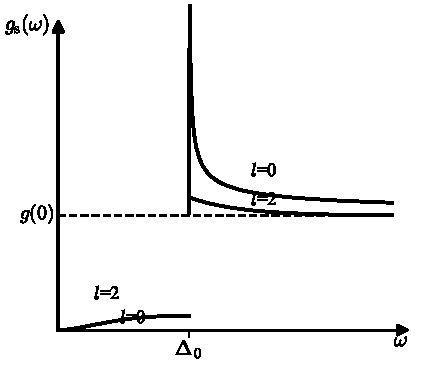
\includegraphics[width=7cm]{fig7-10.pdf}\\{\small 图 7.10\quad s波（$l=0$）与d波（$l=2$）超导体的准粒子态密度}
\end{minipage}
\end{center}

正常金属态密度 $\left[g(0)\right]$ 的趋势.但是，在此低频区域，准粒子的态密度并未消失.这是由于在某些方向上能隙为零，准粒子在节点附近更易于激发，并表现为只要 $\left|\omega\right|>0$ 总存在有限的准粒子态密度，导致在各向异性超导体的准粒子激发谱中不存在真正的能隙.换句话说，与BCS的s波超导体的最明显差别是在 $\left|\omega\right|\ll\Delta_{0}$ 的低频区内仍存在有限的准粒子态密度.

瓦尔玛（Varma）\textsuperscript{[26]}在定性分析了重费密子超导体的低温特性基础上，首先总结出各向异性超导体的低频准粒子态密度 $g_{\mathrm{s}}\sim\left|\omega\right|^{\alpha}$，其中 $\alpha=1$ 代表能隙函数在费密面上具有零线的极向态，$\alpha=2$ 则对应于费密面上存在能隙函数节点的轴向态.显然，图7.10中的d波 $\left(l=2\right)$ 曲线属于轴向态，其低频区态密度正比于 $\omega^{2}$，符合瓦尔玛的幂次规律.为了加深读者对此规律的理解，我们将对p波 $\left(l=1\right)$ 的极向态与轴向态中准粒子的低频态密度作计算：

(i)p波极向态

$\left|\Delta(\hat{\boldsymbol{k}})\right|=\Delta_{0}\left|\cos\theta_{\boldsymbol{k}}\right|$，其中 $\Delta_{0}=\sqrt{3}\,\Delta_{\mathrm{a}}$ 代表最大能隙值（沿 $\theta_{\boldsymbol{k}}=0,\pi$ 方向），在这里赤道线 $\left(\theta_{\boldsymbol{k}}=\dfrac{\pi}{2}\right)$ 为能隙函数的零线，根据式(7.5.4)
\begin{equation*}
  g_{\mathrm{s}}^{\mathrm{polar}}(\omega)=g(0)\frac{\left|\omega\right|}{2}\,\mathrm{Re}
  \int_{-1}^{+1}\mathrm{d}\cos\theta_{\boldsymbol{k}}\,
  \frac{1}{\sqrt{\omega^{2}-\Delta_{0}^{2}\cos^{2}\theta_{\boldsymbol{k}}}}
\end{equation*}
\begin{equation}
\begin{aligned}
  &=\begin{cases}
    g(0)\dfrac{\left|\omega\right|}{2\Delta_{0}}\displaystyle\int_{-1}^{1}\frac{\mathrm{d}x}
    {\sqrt{\left(\dfrac{\omega}{\Delta_{0}}\right)^{2}-x^{2}}} & \left(\left|\omega\right|>\Delta_{0}\right)\\[2em]
    g(0)\dfrac{\left|\omega\right|}{2\Delta_{0}}\,\mathrm{Re}\left[\frac{1}{\mathrm{i}}\int_{-1}^{1}\frac{\mathrm{d}x}
    {\sqrt{x^{2}-\left(\dfrac{\omega}{\Delta_{0}}\right)^{2}}}\right] & \left(\left|\omega\right|<\Delta_{0}\right)
  \end{cases}\\
  &=\begin{cases}
    g(0) & \left(\text{当}\ \left|\omega\right|\gg\Delta_{0}\ \text{时}\right)\\[0.5em]
    g(0)\dfrac{\pi}{2}\cdot\dfrac{\left|\omega\right|}{\Delta_{0}} & \left(\text{当}\ \left|\omega\right|\ll\Delta_{0}\ \text{时}\right)
  \end{cases}
\end{aligned}
\end{equation}
对于“电子型”的准粒子激发，其低频态密度正比于 $\omega$，与瓦尔玛规律一致.在§6中我们还将证明高温超导体的 $d_{x^{2}-y^{2}}$ 配对态也属于存在零线的d波类极向态，其低频态密度也是 $\omega$ 的线性函数.

\subsection*{(ii)p波轴向态}

$\left|\Delta(\hat{\boldsymbol{k}})\right|=\Delta_{0}\left|\sin\theta_{\boldsymbol{k}}\right|$，其中最大能隙值 $\Delta_{0}=\sqrt{\dfrac{3}{2}}\,\Delta_{\mathrm{a}}$，能隙函数的节点在南、北极 $\left(\theta_{\boldsymbol{k}}=0,\pi\right)$ 方向，这时式(7.5.4)可简化为
\begin{equation}
\begin{aligned}
  g_{\mathrm{s}}^{\mathrm{axial}}(\omega)&=g(0)\frac{\left|\omega\right|}{2}\,\mathrm{Re}
  \int_{-1}^{+1}\mathrm{d}\cos\theta_{\boldsymbol{k}}\,
  \frac{1}{\sqrt{\omega^{2}-\Delta_{0}^{2}\sin^{2}\theta_{\boldsymbol{k}}}}\\
  &=g(0)\frac{\left|\omega\right|}{2\Delta_{0}}\ln\left|\frac{\omega+\Delta_{0}}{\omega-\Delta_{0}}\right|\\
  &=\begin{cases}
    g(0) & \left(\text{当}\ \left|\omega\right|\gg\Delta_{0}\ \text{时}\right)\\[0.5em]
    g(0)\left(\dfrac{\omega}{\Delta_{0}}\right)^{2} & \left(\text{当}\ \left|\omega\right|\ll\Delta_{0}\ \text{时}\right)
  \end{cases}
\end{aligned}
\end{equation}
显然，其低频态密度正比于 $\omega^{2}$，也符合瓦尔玛规律.

在各向异性超导体的准粒子态密度曲线中不存在真正的能隙，而是服从 $g_{\mathrm{s}}\left(\left|\omega\right|\ll\Delta_{0}\right)\sim\left|\omega\right|^{\alpha}$（$\alpha=1,2$）的幂次律，这将对其低温超导特征产生重要的影响.

\subsection*{2. 重费密子超导体的低温特性}

在BCS超导体中，由于其态密度曲线中存在能隙，$g_{\mathrm{s}}\left(\left|\omega\right|<\Delta_{0}\right)=0$，$T\ll T_{\mathrm{c}}$ 时的超导准粒子激发应正比于 $\mathrm{e}^{-\beta\Delta_{0}}$，其中 $\Delta_{0}$ 代表零温隙，$\beta=\left(1/k_{\mathrm{B}}T\right)$.因此，在BCS超导体中，一切与准粒子激发有关的物理量，如超导态的低温比热容 $c_{\mathrm{es}}\left(T\ll T_{\mathrm{c}}\right)$［见式(6.5.43)］、穿透深度随温度的变化 $\Delta\lambda\left(T\ll T_{\mathrm{c}}\right)\equiv\lambda(T)-\lambda(0)$［见式(6.8.52)］、低温热导和超声吸收以及反映费密面附近超导准粒子与核磁矩散射的低温核自旋-点阵弛豫率 $T_{1\mathrm{s}}^{-1}\left(T\ll T_{\mathrm{c}}\right)$ 等均已被证实是正比于 $\mathrm{e}^{-\beta\Delta_{0}}$ 的.BCS超导态在 $T\ll T_{\mathrm{c}}$ 时具有指数型的热激发特征标志着这类超导体在费密面上存在着各向同性的能隙.

20世纪80年代初期，在含有稀土（Ce）或锕系（U）元素的金属间化合物中，发现了重费密子系统.这是一种在低温下的重电子（有效质量 $m^{*}=10^{2}\sim10^{3}m_{\mathrm{e}}$）金属材料，实验测出的低温比热容系数 $\gamma$ 和自旋磁化率都比正常金属高2～3个量级.对于重费密子系统的实验研究，展现出十分丰富的物理内容，特别是在这类含磁性离子（如 Ce 与 U）的材料中发现了重费密子超导体.重费密子超导体具有奇异特性，表现为在 $T\ll T_{\mathrm{c}}$ 时的比热容 $c_{\mathrm{es}}(T)$、核自旋-点阵弛豫率 $T_{1\mathrm{s}}^{-1}(T)$、超导与正常态的超声吸收系数比 $\left(\alpha_{\mathrm{S}}/\alpha_{\mathrm{N}}\right)$ 以及伦敦穿透深度随温度的改变等物理量不服从传统BCS超导体的指数型热激发特征 $\mathrm{e}^{-\beta\Delta_{0}}$，而具有温度的简单幂次特征 $T^{n}$，与非声子机制的各向异性的d波配对超导体相类似，具体的实验数值可参看表7.6\textsuperscript{[27,28]}.

表7.6\quad $T\ll T_{\mathrm{c}}$ 时重费密子超导体的特征

\begin{center}\scriptsize
\begin{tabular}{lcccccc}
\hline
重费密子低温 & $\mathrm{CeCu}_{2}\mathrm{Si}_{2}$ & $\mathrm{UBe}_{13}$ & $\mathrm{UPt}_{3}$ & BCS & d波极向态 & d波轴向态\\
超导体特性 & $\left(T_{\mathrm{c}}=0.7\ \mathrm{K}\right)$ & $\left(T_{\mathrm{c}}=1\ \mathrm{K}\right)$ & $\left(T_{\mathrm{c}}=0.5\ \mathrm{K}\right)$ & 超导体 & & \\
\hline
$c_{\mathrm{es}}\left(T\ll T_{\mathrm{c}}\right)$ & $\sim T^{2.8}$ & $\sim T^{2.86}$ & $\sim T^{2}$ & $\sim\mathrm{e}^{-\Delta_{0}/k_{\mathrm{B}}T}$ & $\sim T^{2}$ & $\sim T^{3}$\\
$T_{1\mathrm{s}}^{-1}\left(T\ll T_{\mathrm{c}}\right)$ & $\sim T^{3}$（$^{63}$Cu） & $\sim T^{3}$（$^{9}$Be） & $\sim T^{3}$（$^{195}$Pt） & $\sim T\mathrm{e}^{-\Delta_{0}/k_{\mathrm{B}}T}$ & $\sim T^{3}$ & $\sim T^{5}$\\
$\alpha_{\mathrm{S}}/\alpha_{\mathrm{N}}$ & $?$ & $\sim T^{2}$ & $\sim T^{2}$ & $\sim\mathrm{e}^{-\Delta_{0}/k_{\mathrm{B}}T}$ & $\sim T^{2}$ & $\sim T^{4}$\\
$\Delta\lambda\left(T\ll T_{\mathrm{c}}\right)$ & $\sim T^{2}$ & $\sim T^{2}$ & $\sim T^{2}$ & $\sim\mathrm{e}^{-\Delta_{0}/k_{\mathrm{B}}T}$ &
$\begin{cases}T\left(\mbox{纯}\right)\\ T^{2}\left(\mbox{含杂}\right)\end{cases}$ & $\sim T^{2}$\\
\hline
\end{tabular}
\end{center}

{\emergencystretch 3em
表中的低温比热容和核弛豫率可根据固体物理公式：$c_{\mathrm{es}}\left(T\ll T_{\mathrm{c}}\right)\sim\allowbreak g_{\mathrm{s}}\left(\left|\omega\right|=k_{\mathrm{B}}T\right)\cdot T$ 和 $T_{1\mathrm{s}}^{-1}\left(T\ll T_{\mathrm{c}}\right)\sim\allowbreak g_{\mathrm{s}}\left(\left|\omega\right|=k_{\mathrm{B}}T\right)c_{\mathrm{es}}\left(T\right)$ 作定性估计，其中极向态与轴向态的超导态密度分别正比于 $\omega$ 与 $\omega^{2}$.\par}

仔细分析表7.6中各种重费密子超导体的特征可以看出：$\mathrm{UPt}_{3}$ 基本符合极向态特征，只需假定由于杂质的共振散射效应使极向态的 $\Delta\lambda\left(T\right)$ 正比于 $T^{2}$.至于其它两种重费密子超导体，目前的实验结果还很难断定它们是极向态还是轴向态，尽管较多的数据显示为极向态.在配对的对称性方面，群表示论的研究已证明对于具有立方 $\left(\mathrm{UBe}_{13}\right)$、四角 $\left(\mathrm{CeCu}_{2}\mathrm{Si}_{2}\right)$ 和六角 $\left(\mathrm{UPt}_{3}\right)$ 晶系结构的晶体，在考虑了强自旋-轨道耦合效应后，不存在自旋为三重态配对的p波 $\left(l=1\right)$ 极向态，只可能有自旋单重态配对的d波 $\left(l=2\right)$ 极向态，当然也存在d波轴向态，正是在这个意义上，人们倾向于重费密子超导体是d波超导体.至于是有零线的d波极向态，还是只有节点（零点）的d波轴向态，目前尚难于鉴别，还需要更直接的实验证据.但是，根据重费密子超导体的低温热力学与输运特性服从 $T^{n}$ 幂次律（而不是BCS的指数型 $\mathrm{e}^{-\beta\Delta_{0}}$ 激发规律）的共同特点，至少可以断言：实验表明重费密子超导体是具有非零角动量 $\left(l>0\right)$ 的各向异性超导体.

\section{高温超导体的异常低温特性}

在本章§3中已经指出，铜氧化物高温超导体具有不同于BCS超导体的低温特性，在本节中我们将利用各向异性超导理论，具体求出 $d_{x^{2}-y^{2}}$ 波配对的超导体中低能区准粒子态密度，用于计算 $T\ll T_{\mathrm{c}}$ 时超导态的比热容、伦敦穿透深度和核自旋-点阵弛豫率，并证实在表7.4中所列出的异常低温特性是与 $d_{x^{2}-y^{2}}$ 波配对特征一致的.

\subsection*{1. $d_{x^{2}-y^{2}}$ 波的低频准粒子态密度}

可以将角分辨光电子发射谱（简称ARPES）等实验所证实的 $d_{x^{2}-y^{2}}$ 波能隙函数式(7.3.1)具体写为
\begin{equation}
  \Delta(\hat{\boldsymbol{k}})=\Delta_{0}\cos2\phi\,,\qquad
  \phi=\arctan\left(\hat{k}_{y}/\hat{k}_{x}\right)
\end{equation}
其中 $\hat{k}_{x}$ 与 $\hat{k}_{y}$ 是在平行于 $\mathrm{CuO}_{2}$ 平面的二维BZ中的单位波矢 $\hat{\boldsymbol{k}}$（$\left|\hat{\boldsymbol{k}}\right|=1$）沿x与y轴的分量，$\Delta_{0}$ 代表最大能隙值，而相角 $\phi$ 则从 $k_{x}$ 轴计算.系统在 $d_{x^{2}-y^{2}}$ 波态的超导准粒子态密度可利用式(7.5.4)作计算.将式(7.6.1)代入该式，不难写出在 $0<\omega<\Delta_{0}$ 区域中的态密度为
\begin{equation}
\begin{aligned}
  g_{\mathrm{s}}\left(\omega<\Delta_{0}\right)
  &=g(0)\,\mathrm{Re}\int_{0}^{2\pi}\left(\frac{\mathrm{d}\phi}{2\pi}\right)
  \frac{\omega}{\sqrt{\omega^{2}-\Delta_{0}^{2}\cos^{2}(2\phi)}}\\
  &=g(0)\frac{\left|\omega\right|}{\sqrt{\Delta_{0}^{2}-\omega^{2}}}\left(\frac{2}{\pi}\right)\times\\
  &\quad\mathrm{Re}\int_{0}^{\pi/2}\frac{\mathrm{d}\left(2\phi\right)}
  {\sqrt{\left(\dfrac{\Delta_{0}^{2}}{\Delta_{0}^{2}-\omega^{2}}\right)\sin^{2}(2\phi)-1}}
\end{aligned}
\end{equation}
当 $\omega\ll\Delta_{0}$ 时，可将低频区的态密度近似写为
\begin{equation}
  g_{\mathrm{s}}\left(\omega\ll\Delta_{0}\right)=g(0)\left(\frac{\omega}{\Delta_{0}}\right)\cdot\left(\frac{2}{\pi}\right)\cdot
  \mathrm{Re}\int_{0}^{2\pi}\frac{\mathrm{d}\left(2\phi\right)}{\sqrt{\sin^{2}(2\phi)-1}}
\end{equation}
作变量代换 $2\phi=\mathrm{i}x$，这时 $\sin^{2}(2\phi)=-\sinh^{2}x$，从而得到
\begin{equation}
  g_{\mathrm{s}}\left(\omega\ll\Delta_{0}\right)\approx g(0)\left(\frac{\omega}{\Delta_{0}}\right)\cdot\left(\frac{2}{\pi}\right)\cdot
  \mathrm{Re}\int_{0}^{2\pi}\mathrm{sech}\,x\,\mathrm{d}x\approx g(0)\left(\frac{\omega}{\Delta_{0}}\right)\sim\omega
\end{equation}
在上式中只需取积分的实部，它恰好等于 $\pi/2$.这样就求出了 $d_{x^{2}-y^{2}}$ 波的低频态密度正比于 $\omega$，这个结果与§5中所证明的在三维费密面上存在能隙的零线情况（即极向态）是一致的.在这里我们要提醒读者注意，式(7.6.1)所给出的能隙函数 $\Delta(\hat{\boldsymbol{k}})=\Delta\left(\hat{k}_{x},\hat{k}_{y}\right)$ 是与垂直于 $\mathrm{CuO}_{2}$ 平面方向的动量 $\hat{k}_{z}$ 无关的，这是高温超导铜氧化合物的层状结构所导致的准二维特征.由于相同的原因，系统的三维费密面也具有准二维特征.实际上，能带计算同样表明沿 $k_{z}$ 方向的能带色散可以忽略.因此，系统的三维费密面可以简单看作是二维费密面沿 $k_{z}$ 方向的无色散延伸所构成的柱面.这时，在 $k_{x}$ 与 $k_{y}$ 平面内二维费密面沿 $k_{x}=\pm k_{y}$ 方向的节点在三维动量空间中将构成平行于 $k_{z}$ 方向的零线.因此式(7.6.1)所给出的 $d_{x^{2}-y^{2}}$ 波能隙函数属于在三维费密面上存在零线的d波极向态，其低频准粒子态密度自然具有 $\omega$ 的线性激发特征，并由式(7.6.4)描述.下面将利用此态密度计算氧化物高温超导体的低温物性.

\subsection*{2. $d_{x^{2}-y^{2}}$ 波超导态的低温特性}

低温比热容：从式(6.5.39)出发，类似于s波BCS超导体的低温比热容计算，在 $T\ll T_{\mathrm{c}}$ 时略去该式中 $\beta\left(\mathrm{d}\Delta^{2}/\mathrm{d}\beta\right)$ 项，求得
\begin{equation}
\begin{aligned}
  c_{\mathrm{s}}&\approx2\beta k_{\mathrm{B}}\sum_{k}\hat{\xi}_{k}^{2}
  \left[-\frac{\partial f\left(\hat{\xi}_{k}\right)}{\partial\hat{\xi}_{k}}\right]\\
  &\approx4\beta k_{\mathrm{B}}g(0)\int_{0}^{\infty}\mathrm{d}\varepsilon\,\hat{\xi}^{2}
  \left[-\frac{\partial f(\hat{\xi})}{\partial\hat{\xi}}\right]
  \qquad\left(T\ll T_{\mathrm{c}}\right)
\end{aligned}
\end{equation}
{\emergencystretch 3em
利用在费密面附近正常态与超导态态密度的关系 $g(0)\,\mathrm{d}\varepsilon=\allowbreak g_{\mathrm{s}}(\hat{\xi})\,\mathrm{d}\hat{\xi}$ 以及 $\left[-\partial f/\partial\hat{\xi}\right]=\allowbreak\beta\mathrm{e}^{\beta\hat{\xi}}/\left(\mathrm{e}^{\beta\hat{\xi}}+1\right)^{2}$，可将上式写成\par}
\begin{equation}
\begin{aligned}
  c_{\mathrm{s}}&\approx4\beta^{2}k_{\mathrm{B}}\int_{0}^{\infty}\mathrm{d}\omega\,g_{\mathrm{s}}(\omega)\cdot\omega^{2}\cdot
  \frac{\mathrm{e}^{\beta\omega}}{\left(\mathrm{e}^{\beta\omega}+1\right)^{2}}\\
  &\approx\left(\frac{16k_{\mathrm{B}}}{\beta^{2}\Delta_{0}}\right)\int_{0}^{\infty}\mathrm{d}x\,x^{3}\,\mathrm{sech}^{2}x
  \qquad\left(T\ll T_{\mathrm{c}}\right)
\end{aligned}
\end{equation}
其中 $x=\dfrac{1}{2}\beta\omega$，再利用积分公式 $\int_{0}^{\infty}\mathrm{d}x\,x^{3}\,\mathrm{sech}^{2}x=\left(9/8\right)\zeta(3)$，可求出低温比热容
\begin{equation}
  c_{\mathrm{s}}\left(T\ll T_{\mathrm{c}}\right)\approx18\zeta(3)\left[\frac{g(0)}{\Delta_{0}}\right]k_{\mathrm{B}}^{3}T^{2}\sim T^{2}
\end{equation}
此结果与实验测量一致.若引入线性比热容系数 $\gamma_{\mathrm{s}}(T)\equiv c_{\mathrm{s}}(T)/T$，则求得 $\gamma_{\mathrm{s}}(T)\sim g_{\mathrm{s}}\left(\left|\omega\right|=k_{\mathrm{B}}T\right)\sim T$，可导出表7.6中所用的固体物理学公式 $c_{\mathrm{s}}\left(T\ll T_{\mathrm{c}}\right)\sim g_{\mathrm{s}}\left(\left|\omega\right|=k_{\mathrm{B}}T\right)\cdot T$，这是利用低频区准粒子态密度定性估计低温比热容与温度关系的一个有用公式.

伦敦穿透深度：从式(6.8.50)出发
\begin{equation*}
  \left[\frac{\lambda_{\mathrm{L}}(0)}{\lambda_{\mathrm{L}}(T)}\right]^{2}
  =1-2\beta\int_{0}^{\infty}\mathrm{d}\omega
  \left[\frac{g_{\mathrm{s}}(\omega)}{g(0)}\right]f(\omega)\left[1-f(\omega)\right]
\end{equation*}
考虑到 $T\ll T_{\mathrm{c}}$ 时，$\left[\lambda_{\mathrm{L}}(0)/\lambda_{\mathrm{L}}(T)\right]^{2}-1\approx2\left[\lambda_{\mathrm{L}}(0)-\lambda_{\mathrm{L}}(T)\right]/\lambda_{\mathrm{L}}(0)=-2\Delta\lambda/\lambda_{\mathrm{L}}(0)$，可得到伦敦穿透深度的变化为
\begin{equation}
  \frac{\Delta\lambda\left(T\ll T_{\mathrm{c}}\right)}{\lambda_{\mathrm{L}}(0)}
  \approx\beta\int_{0}^{\infty}\mathrm{d}\omega\,\frac{g_{\mathrm{s}}(\omega)}{g(0)}f(\omega)\left[1-f(\omega)\right]
\end{equation}
将 $d_{x^{2}-y^{2}}$ 波的低频准粒子态密度公式(7.6.4)代入上式，立刻求得
\begin{equation}
\begin{aligned}
  \frac{\Delta\lambda\left(T\ll T_{\mathrm{c}}\right)}{\lambda_{\mathrm{L}}(0)}
  &\approx\beta\int_{0}^{\infty}\mathrm{d}\omega\left(\frac{\omega}{\Delta_{0}}\right)
  \frac{\mathrm{e}^{\beta\omega}}{\left(\mathrm{e}^{\beta\omega}+1\right)^{2}}
  =\left(\frac{k_{\mathrm{B}}T}{\Delta_{0}}\right)\int_{0}^{\infty}\mathrm{d}x\,x\,\mathrm{sech}^{2}x\\
  &=\left(\frac{k_{\mathrm{B}}T}{\Delta_{0}}\right)\ln2\sim T
\end{aligned}
\end{equation}
显然与表7.4中 $\Delta\lambda\left(T\ll T_{\mathrm{c}}\right)\sim T$ 的实验结果一致，说明高温超导体属于 $d_{x^{2}-y^{2}}$ 波配对的超导态.最后再看 $T_{1\mathrm{s}}^{-1}$ 的计算结果：

核自旋-点阵弛豫率：可直接利用固体物理的定性公式，由低频态密度与低温比热容求出
\begin{equation}
  T_{1\mathrm{s}}^{-1}\left(T\ll T_{\mathrm{c}}\right)\sim g_{\mathrm{s}}\left(\left|\omega\right|=k_{\mathrm{B}}T\right)\cdot c_{\mathrm{s}}\left(T\ll T_{\mathrm{c}}\right)\sim T^{3}
\end{equation}
它也与表7.4中所列出的测量结果定性相符.

总之，在铜氧化合物高温超导体中，$T\ll T_{\mathrm{c}}$ 时超导态中物理特性的实验结果与ARPES和SQUID等方法确定的 $d_{x^{2}-y^{2}}$ 波超导态特征是相吻合的，进一步证实了这类超导体是能隙函数存在零线的d波各向异性配对超导体.高温超导体在配对对称性的研究方面已经比较早发现的重费密子超导体更为深入和确定了.

\subsection*{3. $d_{x^{2}-y^{2}}$ 波超导态的零温能隙与$T_{\mathrm{c}}$之比值}

从各向异性超导体的有限温度能隙方程式(7.4.28)出发，取 $d_{x^{2}-y^{2}}$ 波的二维超导能隙函数公式(7.6.1)
\begin{equation*}
  \Delta\left(\hat{\boldsymbol{k}},T\right)=\Delta_{0}(T)\cos2\phi\,,\qquad
  \phi=\arctan\left(\hat{k}_{y}/\hat{k}_{x}\right)
\end{equation*}
相应的在二维平面中的吸引势取为
\begin{equation}
  V\left(\hat{\boldsymbol{k}}\cdot\hat{\boldsymbol{k}}'\right)=-V_{\mathrm{d}}\cos\left[2\left(\phi-\phi'\right)\right]
  \qquad\left(V_{\mathrm{d}}>0\right)
\end{equation}
这时 $d_{x^{2}-y^{2}}$ 波的二维能隙方程变为
\begin{equation*}
\begin{aligned}
  \Delta_{0}(T)\cos(2\phi)
  &=V_{\mathrm{d}}\cos(2\phi)\sum_{k'}
  \frac{\cos^{2}(2\phi')\tanh\left(\dfrac{1}{2}\beta\hat{\xi}_{k'}\right)}{2\hat{\xi}_{k'}}\\
  &\quad+V_{\mathrm{d}}\sin(2\phi)\sum_{k'}
  \frac{\cos(2\phi')\sin(2\phi')\tanh\left(\dfrac{1}{2}\beta\hat{\xi}_{k'}\right)}{2\hat{\xi}_{k'}}
\end{aligned}
\end{equation*}
其中
\begin{equation}
  \hat{\xi}_{k'}\equiv\left[\varepsilon_{k'}^{2}+\left|\Delta_{0}(T)\cos(2\phi')\right|^{2}\right]^{1/2}
\end{equation}
由于在二维能隙方程的等式右边第二项是 $\phi'$ 的奇函数，当对 $\hat{\boldsymbol{k}}'$ 作求和时此项应为零，从而可求得与式(7.4.30a)相应的 $d_{x^{2}-y^{2}}$ 波自洽方程：
\begin{equation}
  1=V_{\mathrm{d}}\sum_{k'}\frac{\cos^{2}(2\phi')\tanh\left(\dfrac{1}{2}\beta\hat{\xi}_{k'}\right)}{2\hat{\xi}_{k'}}
\end{equation}
由此可具体计算 $\Delta_{0}(0)$ 与 $T_{\mathrm{c}}$.

零温能隙：
\begin{equation*}
\begin{aligned}
  1&=\frac{1}{2}V_{\mathrm{d}}\sum_{k'}
  \frac{\cos^{2}(2\phi')}{\sqrt{\varepsilon_{k'}^{2}+\Delta_{0}^{2}(0)\cos^{2}(2\phi')}}\\
  &=\frac{1}{2}g(0)V_{\mathrm{d}}\int_{0}^{2\pi}\frac{\mathrm{d}\phi}{2\pi}
  \int_{-\hbar\omega_{0}}^{\hbar\omega_{0}}\mathrm{d}\varepsilon\,
  \frac{\cos^{2}(2\phi)}{\sqrt{\varepsilon^{2}+\Delta_{0}^{2}(0)\cos^{2}(2\phi)}}\\
  &=g(0)V_{\mathrm{d}}\int_{0}^{2\pi}\frac{\mathrm{d}\phi}{2\pi}\cos^{2}(2\phi)
  \ln\left[\frac{2\hbar\omega_{0}}{\Delta_{0}(0)\left|\cos(2\phi)\right|}\right]
\end{aligned}
\end{equation*}
其中考虑了弱耦合超导理论中的近似条件 $\Delta_{0}(T)\ll\hbar\omega_{0}$，因此零温时最大能隙 $\Delta_{0}(0)$ 满足方程
\begin{equation*}
  1=\frac{1}{2}g(0)V_{\mathrm{d}}\ln\left[2\Gamma\hbar\omega_{0}/\Delta_{0}(0)\right]
\end{equation*}
由此求出
\begin{equation*}
  \Delta_{0}(0)=\left(2\hbar\omega_{0}\right)\Gamma\exp\left[\frac{-1}{\dfrac{1}{2}g(0)V_{\mathrm{d}}}\right]
\end{equation*}
其中
\begin{equation*}
\begin{aligned}
  \ln\Gamma&\equiv-\left(\frac{4}{\pi}\right)\int_{0}^{\pi/2}\mathrm{d}\left(2\phi\right)\cos^{2}(2\phi)\ln\cos(2\phi)\\
  &=-\left(4/\pi\right)\int_{0}^{1}\mathrm{d}x\,x^{2}\ln x/\sqrt{1-x^{2}}=\ln\left(\frac{2}{\sqrt{\mathrm{e}}}\right)
\end{aligned}
\end{equation*}
在这里 $x\equiv\cos(2\phi)$，零温时 $d_{x^{2}-y^{2}}$ 波的最大能隙为
\begin{equation}
\begin{aligned}
  &\Delta_{0}(0)=\Gamma\cdot\left(2\hbar\omega_{0}\right)\exp\left[\frac{-1}{\dfrac{1}{2}g(0)V_{\mathrm{d}}}\right]\\
  &\Gamma=2/\sqrt{\mathrm{e}}>1
\end{aligned}
\end{equation}
至于在零温时 $d_{x^{2}-y^{2}}$ 波的平均能隙 $\Delta_{\mathrm{a}}(0)$，根据式(7.4.37)与(7.4.38)，应满足条件：
\begin{equation}
  \Delta_{\mathrm{a}}^{2}(0)=\int_{0}^{2\pi}\frac{\mathrm{d}\phi}{2\pi}\Delta_{0}^{2}(0)\cos^{2}(2\phi)
  =\frac{1}{2}\Delta_{0}^{2}(0)
\end{equation}
因此 $\Delta_{\mathrm{a}}(0)=\Delta_{0}(0)/\sqrt{2}$，其解析表示式为
\begin{equation}
\begin{aligned}
  &\Delta_{\mathrm{a}}(0)=Q\cdot\left(2\hbar\omega_{0}\right)\exp\left[\frac{-1}{\dfrac{1}{2}g(0)V_{\mathrm{d}}}\right]\\
  &Q=\sqrt{\left(2/\mathrm{e}\right)}<1
\end{aligned}
\end{equation}
与式(7.4.44)所给出的一般性结论 $Q<1$ 相符合.

转变温度 $T_{\mathrm{c}}$：可从有限温度的自洽方程式(7.6.13)出发，考虑到 $T=T_{\mathrm{c}}$ 时能隙 $\Delta_{0}\left(T_{\mathrm{c}}\right)=0$，求出
\begin{equation*}
\begin{aligned}
  1&=g(0)V_{\mathrm{d}}\left[\int_{0}^{2\pi}\frac{\mathrm{d}\phi}{2\pi}\cos^{2}(2\phi)\right]
  \int_{0}^{\hbar\omega_{0}}\mathrm{d}\varepsilon\,\frac{\tanh\left(\varepsilon/2k_{\mathrm{B}}T_{\mathrm{c}}\right)}{\varepsilon}\\
  &=\frac{1}{2}g(0)V_{\mathrm{d}}\ln\left[\left(\frac{2\mathrm{e}^{\gamma}}{\pi}\right)\left(\frac{\hbar\omega_{0}}{k_{\mathrm{B}}T_{\mathrm{c}}}\right)\right]
\end{aligned}
\end{equation*}
因此
\begin{equation}
  k_{\mathrm{B}}T_{\mathrm{c}}=\left(2\mathrm{e}^{\gamma}/\pi\right)\hbar\omega_{0}\exp\left[\frac{-1}{\dfrac{1}{2}g(0)V_{\mathrm{d}}}\right]
\end{equation}
由此求得在弱耦合情形 $d_{x^{2}-y^{2}}$ 波配对的零温最大能隙与 $T_{\mathrm{c}}$ 之比值为
\begin{equation}
  \left[2\Delta_{0}(0)/k_{\mathrm{B}}T_{\mathrm{c}}\right]=\left(2\pi\mathrm{e}^{-\gamma}\right)\Gamma=4.28
  \qquad\left(\Gamma=2/\sqrt{\mathrm{e}}>1\right)
\end{equation}
它略大于BCS弱耦合超导体的标准值3.53，但是弱耦合 $d_{x^{2}-y^{2}}$ 波的零温平均能隙 $\Delta_{\mathrm{a}}(0)$ 与 $T_{\mathrm{c}}$ 之比值则为
\begin{equation}
  \left[2\Delta_{\mathrm{a}}(0)/k_{\mathrm{B}}T_{\mathrm{c}}\right]=\left(2\pi\mathrm{e}^{-\gamma}\right)Q=3.03
  \qquad\left(Q=\sqrt{2/\mathrm{e}}<1\right)
\end{equation}
它总是小于3.53，与式(7.4.45)一致.以上两个特征性比值都可以用作判断铜氧化合物高温超导体是否属于弱耦合情形.早期的实验测量多半是用陶瓷或多晶样品，所测得的比值应代表平均能隙 $2\Delta_{\mathrm{a}}(0)$ 与 $k_{\mathrm{B}}T_{\mathrm{c}}$ 之比，其实测值往往大于5.近年来由于实验技术的发展，已能在良好制备的单晶中较准确的测量最大能隙 $\Delta_{0}$，实验给出的 $2\Delta_{0}(0)$ 与 $T_{\mathrm{c}}$ 之比值在8～9之间，也明显超出了式(7.6.18)所规定的范围.因此，无论从最大能隙或者从平均能隙与 $T_{\mathrm{c}}$ 之比值的实验结果来判断，高温超导体都不能用弱耦合描述，而必须采用强耦合的超导理论.

\section{高温超导体正常态的反常特征（最佳化合物）}

众所周知，在电声子机制的BCS超导体中，$T>T_{\mathrm{c}}$ 时的正常态是普通的金属态，并且完全可以用标准的朗道费密液体理论描述.正由于对费密液体有比较深入的了解，BCS等人从费密面附近一对动量和自旋取向相反的电子间通过声子传递有效的吸引作用可以导致费密球态失稳的特征，提出了常规超导体中配对吸引来源于电子与声子的相互作用，简称配对的声子机制.因此，为了探明形成超导的微观机制，必须对 $T>T_{\mathrm{c}}$ 正常态的特性有比较清楚的了解.人们自然会问，在铜氧化合物中 $T>T_{\mathrm{c}}$ 时的金属性正常态是否仍然属于费密液体？大量的实验结果表明其正常态的许多物理性质，例如 $T>T_{\mathrm{c}}$ 时的直流电阻率、光电导以及核磁共振（NMR）中的自旋-点阵弛豫率等，均与普通金属行为很不相同，表现出十分异常的奇特行为，而且均不能用标准的朗道费密液体理论描述，这就是人们通常所说的高温超导体正常态的反常特征.限于篇幅，我们仅选择几个主要的实验事实来说明其正常态的反常，详细的讨论可参考文献\textsuperscript{[29]}.在本节中我们主要介绍最佳化合物正常态的非费密液体行为，而在下节中再介绍在弱掺杂区中新近发现的正常态能隙等奇异现象.

早期对正常态特征的研究多集中于讨论具有最高超导转变温度 $T_{\mathrm{c}}=T_{\mathrm{c}}^{\mathrm{max}}$ 的最佳化合物，如 $\mathrm{La}_{2-x}\mathrm{Sr}_{x}\mathrm{CuO}_{4}$（$x\approx0.15$）及 $\mathrm{YBa}_{2}\mathrm{Cu}_{3}\mathrm{O}_{6+x}$（$x\approx1$）等的输运性质及核磁共振谱的反常.高温超导体正常态最为突出的反常特征是在最简单的直流电阻率 $\rho_{\mathrm{ab}}$ 的测量中被发现的，这里的 $\rho_{\mathrm{ab}}$ 代表沿导电层（即 $\mathrm{CuO}_{2}$ 平面）方向的正常态电阻率.对于所有的铜氧化合物高温超导体，在最佳掺杂（即最佳化合物）情况下，正常态的一个重要反常特征是

\subsection*{1. $\rho_{\mathrm{ab}}$普遍地具有线性温度行为}

大量的实验报道证实，所有最佳化合物沿导电层的直流电阻率均随温度升高而线性增大，其线性温区可从下界温度 $T_{\mathrm{c}}$ 一直延伸到很高的上界温度 $T_{\mathrm{max}}$.对于 $x=0.15$ 的掺杂（Sr）La-214 系统，$T_{\mathrm{max}}=1\,000$ K，而Y-123 和 Bi-2212 最佳化合物也可以延伸到600 K.特别值得指出的是，Bi-2201（$\mathrm{Bi}_{2}\mathrm{Sr}_{2}\mathrm{CuO}_{6}$）由于 $T_{\mathrm{c}}$（约为7 K）很低，其 $\rho_{\mathrm{ab}}$ 的线性温度关系在7～700 K的宽阔温区内都成立.线性温区的下界温度可以低于10 K是正常态电阻率反常的一个重要特点.

最佳化合物的正常态 $\rho_{\mathrm{ab}}$ 可用下列公式描述：
\begin{equation}
  \rho_{\mathrm{ab}}(T)=\alpha T+\rho_{0}
\end{equation}
其中 $\alpha$ 是线性温度关系的斜率，$\rho_{0}$ 为将 $\rho_{\mathrm{ab}}(T)$ 的线性关系外延到绝对零度时的插值，也可称为“剩余电阻率”.随着样品质量的不断提高，测出的 $\rho_{0}$ 值越来越小，可以认为，高质量样品的 $\rho_{0}$ 值将趋于零，这时表征 $\rho_{\mathrm{ab}}(T)$ 的物理参数只是 $\alpha$.图7.11中给出了几种高温超导体正常态的 $\rho_{\mathrm{ab}}(T)$ 曲线，其中除了Y-123（60 K）样品外，其它均为最佳化合物，虽然它们的具体结构有很大差异，但它们在 $T_{\mathrm{c}}$ 之上的 $\rho_{\mathrm{ab}}$ 曲线却均具有近似的线性行为，而且 $\alpha$ 的数值也很相近.至于图7.11中的 Y-123（60 K）材料是 $T_{\mathrm{c}}=60$ K 的 $\mathrm{YBa}_{2}\mathrm{Cu}_{3}\mathrm{O}_{6+x}$（$x=0.6\sim0.7$）样品，属于弱（或欠）掺杂的Y-123系统，其 $\rho_{\mathrm{ab}}$ 曲线在 $T_{\mathrm{c}}$ 以上的一段温区内明显地偏离线性规律是由于在正常态中形成了能隙，我们将在§8中再作讨论.

应当明白，在7～1000 K这样广阔的温度范围内，沿导电层的电阻率 $\rho_{\mathrm{ab}}$ 与温度成线性关系是十分异常的现象，它与普通金属的 $\rho$-$T$ 特征判然有别.在普通金属中，电阻率随温度的变化主要来源于电声子散射.熟习固体物理学的读者都知道，来源于电子-声子散射的金属电阻率由布洛赫-格林艾森（Bloch-Grüneisen）公式（以下简称B-G公式）\textsuperscript{[30]}描述，在三维系统中B-G公式可以写为
\begin{equation}
  \rho(T)=A\left(T/\theta_{\mathrm{D}}\right)^{5}\int_{0}^{\theta_{\mathrm{D}}/T}\mathrm{d}z\,
  \frac{z^{5}}{\left(\mathrm{e}^{z}-1\right)\left(1-\mathrm{e}^{-z}\right)}
  \sim\begin{cases}T & \left(T\gg\theta_{\mathrm{D}}\right)\\[0.3em]
  T^{5} & \left(T\ll\theta_{\mathrm{D}}\right)\end{cases}
\end{equation}

\begin{center}
\begin{minipage}{9cm}
\centering
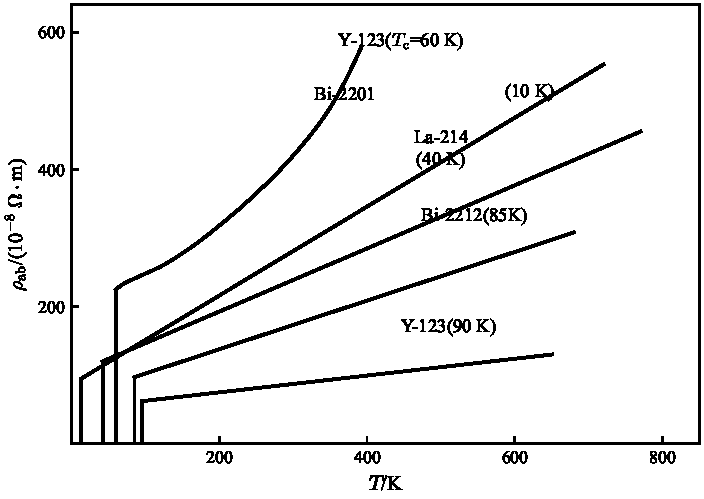
\includegraphics[width=9cm]{fig7-11.pdf}\\{\small 图 7.11\quad 几种高温超导体正常态的 $\rho_{\mathrm{ab}}(T)$ 曲线}
\end{minipage}
\end{center}

其中 $\theta_{\mathrm{D}}$ 是德拜温度，对于普通金属大约在200～400 K之间，而对于铜氧化合物高温超导体 $\theta_{\mathrm{D}}$ 的取值也不低于200 K.B-G公式所预言的在 $T\ll\theta_{\mathrm{D}}$ 低温区 $\rho\sim T^{5}$ 和在室温附近的 $\rho\sim T$ 线性关系是人们早已熟知的定性概念.若进一步对B-G公式作定量的计算，其结果与普通金属中电阻率的测量数据符合良好，如图7.12所示.从图中可以看出，实际上普遍金属电阻率的线性温度区可以放宽到 $T>\left(\theta_{\mathrm{D}}/5\right)$，约在40 K以上，$\left(\theta_{\mathrm{D}}/5\right)$ 可作为线性温区的下界，低于此下界温度应当进入电声子机制电阻率的非线性温度区.但是 Bi-2201 中的线性温度区下界可延续到10 K以下，远低于电声子机制中线性区的下界（40 K），导致在B-G公式的非线性区域中出现反常的线性行为，从而对电声子机制对于铜氧化合物的适用性提出了严重的挑战.此外，在 $T\ll\theta_{\mathrm{D}}$ 的低温区中，迄今尚未观察到在铜氧化物中出现 $\rho\sim T^{5}$（三维）或 $T^{4}$（二维）的行为.这些结果都不能用电子被声子散射来解释.另一方面，在普通金属中还存在电阻率的高温饱和现象，其物理原因是随着温度T的升高，电子与声子的散射效应将不断地增强，导致载流子平均自由程不断地减小，而平均自由程有一个下限，它不能小于近邻原子的间距，此即著名的约飞（Ioffe）判据，这个下限的存在导致电声子散射机制的电阻率在高温时趋向于饱和.文献\textsuperscript{[31]}用 Cu-O 键长作为电子被声子散射平均自由程的下限，定性地估计了铜氧化合物中电声子机制的饱和电阻率约为1 $\mathrm{m\Omega\cdot cm}$，然而在最佳掺杂的 La-214 系统中线性温区可高达1000 K，所对应的 $\rho_{\mathrm{ab}}$ 值早已超过1 $\mathrm{m\Omega\cdot cm}$（如图7.16所示），却未见饱和迹象，这也是电声子机制不能解释的.

\begin{center}
\begin{minipage}{7.5cm}
\centering
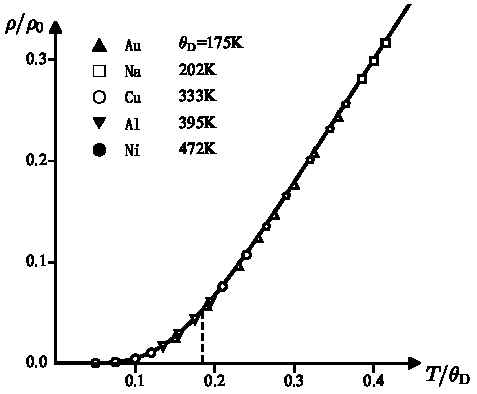
\includegraphics[width=7.5cm]{fig7-12.pdf}\\{\small 图 7.12\quad 几种简单金属的电阻率-温度曲线}\\[0.2em]
{\small （其中实线代表B-G公式的定量计算曲线）}
\end{minipage}
\end{center}

综上所述，正常态电阻率在异常宽的温度范围内满足线性规律实际上已排除了声子作为载流子散射主要来源的可能性，我们有理由认为，在高温超导体正常态中的电阻率反常不是电子-声子散射所造成的.为了解释 $\rho_{\mathrm{ab}}$ 的普适线性温度行为，应当寻找新的散射机制，而探明产生电阻反常的原因，必将有助于解开高温超导电性之谜.历史上在BCS常规超导体中，正是同一种相互作用（电声子耦合）既产生正常态的电阻，又导致在 $T\leqslant T_{\mathrm{c}}$ 时失去电阻和形成超导电性.

此外，在良好制备的Y-123最佳化合物中，从直流电阻率 $\rho_{\mathrm{ab}}(T)$ 的倒数求出的直流（静态）导电率 $\sigma_{\mathrm{ab}}(T)=1/\rho_{\mathrm{ab}}(T)$ 也与从光学（动态）导电率 $\sigma_{\mathrm{ab}}(\omega,T)$ 测量所得到的零频极限 $\sigma_{\mathrm{ab}}(\omega=0,T)$ 值定量相符.这使得人们可以组合两种测量数据，导出一个唯象公式，用于统一描述高温超导体正常态的动态与静态电导特征.

\subsection*{2. 解释光电导率反常的一个唯象公式}

利用光在单晶上垂直入射的反射比 $R(\omega)$ 的测量，可以在很宽的光子能量范围提供金属中动态导电率 $\sigma(\omega)$ 的重要信息.这是因为光的垂直入射的反射比，根据式(2.7.17)，可表示为
\begin{equation}
  R(\omega)=\left|\frac{\sqrt{\varepsilon(\omega)}-1}{\sqrt{\varepsilon(\omega)}+1}\right|^{2}
\end{equation}
其中 $\varepsilon(\omega)$ 是金属的介电函数，而在金属中 $\varepsilon(\omega)$ 与光导电率 $\sigma(\omega)$ 是密切相关的物理量，并且在固体物理学中已经介绍了\textsuperscript{[32]}它们的关系式
\begin{equation}
  \varepsilon(\omega)=1+\mathrm{i}\,4\pi\sigma(\omega)/\omega
\end{equation}
和描述光导电率的特鲁德（Drude）公式
\begin{equation}
  \sigma(\omega)=\frac{\omega_{\mathrm{p}}^{2}\tau/4\pi}{1-\mathrm{i}\omega\tau}
\end{equation}
这里 $\omega_{\mathrm{p}}$ 是等离激元的频率，对于球形费密面 $\omega_{\mathrm{p}}^{2}=\left(4\pi ne^{2}/m^{*}\right)$，其中 n 与 $m^{*}$ 分别代表载流子浓度和有效质量.上式中 $\tau$ 是一个唯象参数，称为弛豫时间，其倒数 $\left(1/\tau\right)$ 则代表载流子每秒被散射的概率，简称散射率.式(7.7.3)—(7.7.5)给出了从反射比测量提供光电导率信息的具体关系式.

从特鲁德公式(7.7.5)还可以看出，光导电率 $\sigma(\omega)$ 的零频极限（$\omega=0$）就是熟知的直流导电率公式 $\sigma_{\mathrm{dc}}=\sigma(0)=\omega_{\mathrm{p}}^{2}\tau/4\pi\left(=ne^{2}\tau/m^{*}\right)$.另外，在 $\sigma_{\mathrm{dc}}$ 的测量中只能获取 $\omega_{\mathrm{p}}^{2}$ 与 $\tau$ 乘积的实验数据，而无法将两者分开.但是 $\sigma(\omega)$ 的测量却能将 $\omega_{\mathrm{p}}^{2}$ 与 $\tau$ 这两个因子分开，例如当 $\omega\tau\gg1$ 时，$\sigma(\omega)\approx\mathrm{i}\left(\omega_{\mathrm{p}}^{2}/4\pi\omega\right)$，代入式(7.7.4)求得熟知的金属介电函数的高频近似式
\begin{equation}
  \varepsilon(\omega)=1-\frac{\omega_{\mathrm{p}}^{2}}{\omega^{2}}\qquad\left(\omega\tau\gg1\right)
\end{equation}
显然当 $\omega<\omega_{\mathrm{p}}$ 时，$\varepsilon(\omega)<0$ 是一个负数，代入反射比公式(7.7.3)，求得 $R\left(\omega<\omega_{\mathrm{p}}\right)=1$ 的全反射情形.当 $\omega>\omega_{\mathrm{p}}$ 时，$\varepsilon(\omega)$ 为正实数，$R(\omega)<1$，这时光才可以在金属中传播，并使金属成为透明的，实验上已观测到碱金属在紫外区具有透明性，$\omega_{\mathrm{p}}$ 是反射区的上界.因此，$\omega_{\mathrm{p}}$ 的实验值可以从反射区上界直接确定，从而通过光电导率的测量又可获取散射率 $\left(1/\tau\right)$ 的实验信息，并拟合出适用于远红外 $\left(\hbar\omega<0.07\ \mathrm{eV}\right)$ 和中红外区 $\left(\hbar\omega<0.5\ \mathrm{eV}\right)$ 的唯象公式.

图7.13给出从光反射比测量所得到的 $\mathrm{YBa}_{2}\mathrm{Cu}_{3}\mathrm{O}_{7}$（$T_{\mathrm{c}}=90$ K）最佳化合物光电导率之实部 $\sigma_{1}\left(\omega,T\right)$，图中的实线分别为 $T=100$ K 与 200 K 时的实验曲线.实验结果可以看成是由两部分组成\textsuperscript{[29]}：其中之一为出现在远红外区 $\left(\hbar\omega<0.07\ \mathrm{eV}\right)$ 的尖峰部分，该峰以 $\omega=0$ 为中心，尖峰的高度对应于直流电导率，而峰的半宽度略小于 $2k_{\mathrm{B}}T$.另一部分是 $\sigma_{1}$ 随 $\omega$ 相对平坦变化的部分，又称为平台部分，主要出现在中红外区 $\left(\hbar\omega<0.5\ \mathrm{eV}\right)$.为了和特鲁德公式作比较，可写出式(7.7.5)的实部
\begin{equation}
  \sigma_{1}(\omega)=\mathrm{Re}\,\sigma(\omega)=\frac{\omega_{\mathrm{p}}^{2}\tau/4\pi}{1+\omega^{2}\tau^{2}}
\end{equation}

\begin{center}
\begin{minipage}{8.5cm}
\centering
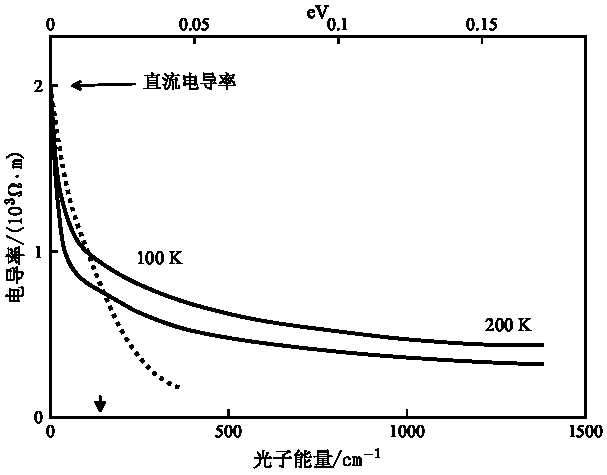
\includegraphics[width=8.5cm]{fig7-13.pdf}\\{\small 图 7.13\quad $\mathrm{YBa}_{2}\mathrm{Cu}_{3}\mathrm{O}_{7}$ 晶体的 $\sigma_{1}(\omega,T)$ 曲线，}\\[0.2em]
{\small 其中实线为实验曲线，点线是特鲁德公式的拟合，箭头表示的能量为 $k_{\mathrm{B}}\times200$ K}
\end{minipage}
\end{center}

显然，特鲁德公式也给出以 $\omega=0$ 为中心的尖峰，其峰的半宽度相当的光子 $\hbar\omega$ 应为 $\left(\hbar/\tau\right)$.为了再现远红外区的尖峰行为，可取 $\left(\hbar/\tau\right)\approx2k_{\mathrm{B}}T$ 作为一个初步的拟合.在图7.13中的点线是取 $T=100$ K 时特鲁德公式的拟合曲线，它与 $T=100$ K 的实验曲线在 $\hbar\omega<k_{\mathrm{B}}T$ 区内符合良好.在 $T=200$ K 的实验曲线左边的点线则是取 $T=200$ K 的特鲁德拟合曲线，它与实线在低频端的延伸也是一致的.这表明利用特鲁德公式作 $\left(\hbar/\tau\right)\approx2k_{\mathrm{B}}T$ 的简单拟合可以说明 $\sigma_{1}\left(\omega,T\right)$ 的尖峰行为.但是这个简单的拟合不能外推到 $\hbar\omega\gg k_{\mathrm{B}}T$ 的中红外区，在那里，$T=100$ K 的实验曲线与同一温度的特鲁德拟合曲线（点线）偏离较大，实验曲线的下降比特鲁德公式要缓慢得多.这表明 $\left(\hbar/\tau\right)\approx2k_{\mathrm{B}}T$ 拟合至少是不全面的，它没有反映出中红外区的平台特征.为了反映光电导谱的平台特征，人们采用了推广的特鲁德公式，即在式(7.7.7)基础上引入随频率 $\omega$ 变化的散射率 $1/\tau\left(\omega,T\right)$，用于拟合实验的 $\sigma\left(\omega,T\right)$ 曲线.一个与实验 $\sigma\left(\omega,T\right)$ 曲线良好符合的散射率公式是 $\hbar/\tau\left(\omega,T\right)=0.6\left(\pi k_{\mathrm{B}}T+\hbar\omega\right)$，等式右边第一项与简单拟合相近，既可以说明远红外区的尖峰特征，又可以再现 $\omega=0$ 时直流电阻率的测量值，新增加的第二项是散射率随 $\omega$ 的线性增长项，将阻止特鲁德导电率随 $\omega$ 增加而下降的趋势，形成中红外区 $\sigma_{1}$ 的平台特征.为了定性解释远红外与中红外区的光导电谱特征，通常采用一个比较宽松的唯象公式
\begin{equation}
  \left(\hbar/\tau\right)^{2}=\left(Ak_{\mathrm{B}}T\right)^{2}+\left(B\hbar\omega\right)^{2}
\end{equation}
式中A和B是数量级为1的常量.从上式不难看出，当 $\hbar\omega\ll k_{\mathrm{B}}T$ 时 $\left(\hbar/\tau\right)\sim k_{\mathrm{B}}T$，反之当 $\hbar\omega\gg k_{\mathrm{B}}T$ 时 $\left(\hbar/\tau\right)\sim\hbar\omega$，表明尖峰与平台特征均已纳入到这个唯象公式之中了.应当指出，在低温时从唯象公式导出的 $\left(1/\tau\right)\sim\omega$ 具有重要的物理内涵，其中 $\tau$ 是弛豫时间，在固体物理学中它是载流子的漂移速度按照 $v_{\mathrm{d}}(t)=v_{\mathrm{d}}(0)\mathrm{e}^{-t/\tau}$ 的指数规律衰减的特征时间，在相互作用的电子体系中（见第四章§11），这个 $\tau$ 也可称作准粒子（空穴或电子）的寿命，其倒数正比于准粒子自能的虚部.因此，可以从光电导实验的拟合求得高温超导体正常态的准粒子自能虚部正比于频率，即 $\mathrm{Im}\,\Sigma\sim\omega$，自能虚部的这一特征完全不同于普通金属所具有的朗道费密液体特征.对于朗道费密液体，在低温时根据式(4.11.15)，费密面附近的自能虚部 $\mathrm{Im}\,\Sigma_{\mathrm{FL}}\sim\omega^{2}$，其中取费密面为能量的原点.由此可知，铜氧化物在 $T_{\mathrm{c}}$ 之上的金属性正常态不能用朗道的费密液体理论描述.正是在这个意义上，人们常说高温超导体的正常态可能是一种非费密液体状态.

\subsection*{3. 核自旋-点阵弛豫率的反常}

核磁共振实验中的自旋-点阵弛豫率 $T_{1}^{-1}$ 是表征核自旋磁化强度 $\boldsymbol{M}(t)$ 从偏离平衡（由于外磁场的突然撤除与接入）的状态趋向于平衡值 $\boldsymbol{M}_{0}$ 的速率
\begin{equation}
  \frac{\mathrm{d}M(t)}{\mathrm{d}t}=\frac{\left[M_{0}-M(t)\right]}{T_{1}}
\end{equation}
或者用于描述 $M(t)$ 解的时间演化规律
\begin{equation}
  \left|M(t)-M_{0}\right|\sim\exp\left(\frac{-t}{T_{1}}\right)
\end{equation}
其中 $T_{1}$ 又称为自旋-点阵弛豫时间.这里人们用“自旋-点阵”术语是由于弛豫的机制来源于核自旋系统与点阵晶格系统之间的散射互作用.这是一种测量磁响应的有力工具，它可以提供晶体中不同核自旋的格点上电子态的信息.例如，在铜氧化合物高温超导体中，通过对导电层平面上 $^{63}\mathrm{Cu}$ 与 $^{17}\mathrm{O}$ 等格点上核弛豫率 $T_{1}^{-1}$ 的测量，可以提供其超导与正常态电子特征的重要信息.

在金属晶格中，核自旋与传导电子（属于点阵系统）之间的散射是产生自旋-点阵弛豫的主要机制.在朗道费密液体理论中，由于费密面的存在，必然导致正常金属的 $T_{1}^{-1}$ 正比于T，或 $T_{1}(T)\cdot T=$ 常数的柯林嘎（Korringa）关系.在推导此关系时，应当注意一个重要的差别，即核磁矩在磁场中的能级分裂 $\left(E_{m}-E_{n}\right)$ 远远小于电子自旋矩的相应能级分裂，这是由于质子质量比电子重1836倍，相应的核磁子 $\mu_{\mathrm{n}}$ 将比电子的玻尔磁子 $\mu_{\mathrm{B}}$ 要小相同的倍数.

现在简要介绍，在普通金属中柯林嘎关系的理论推导.核自旋与传导电子之间的相互作用由接触势描述，它与第十一章中将要介绍的局域自旋与传导电子间的 s-d（或 s-f）交换作用十分相似，可写成
\begin{equation}
  H_{\mathrm{int}}=V\cdot\boldsymbol{I}\cdot\hat{\boldsymbol{\sigma}}
\end{equation}
其中 $\boldsymbol{I}$ 是核自旋，$\hat{\boldsymbol{\sigma}}$ 为传导电子自旋泡利矩阵的矢量表示式，而V代表这个接触势的互作用强度.核自旋系统与传导电子的散射过程如图7.14所示.

当发生散射时，核自旋将偏转而在其磁场分裂能级 $E_{m}$ 与 $E_{n}$ 之间跳跃，这时电子的动量 k 与自旋s也将改变.当核自旋从量子态m跃迁到n的同时，传导电子将从初态 $\left|\boldsymbol{k},s\right\rangle$ 散射到终态 $\left|\boldsymbol{k}',s'\right\rangle$，所对应的电子能量分别为 $\varepsilon_{ks}$ 与 $\varepsilon_{k's'}$.核自旋-点阵的弛豫率可利用 $H_{\mathrm{int}}$ 的二级微扰理论写出
\begin{equation}
\begin{aligned}
  T_{1}^{-1}(T)&\sim\frac{2\pi}{\hbar}\sum_{k,k'}\sum_{s,s'}
  \left|\left\langle m,\boldsymbol{k},s\mid V\mid n,\boldsymbol{k}',s'\right\rangle\right|^{2}
  f\left(\varepsilon_{ks}\right)\times\\
  &\quad\left[1-f\left(\varepsilon_{k's'}\right)\right]\cdot
  \delta\left(E_{m}-E_{n}+\varepsilon_{ks}-\varepsilon_{k's'}\right)
\end{aligned}
\end{equation}

\begin{center}
\begin{minipage}{6cm}
\centering
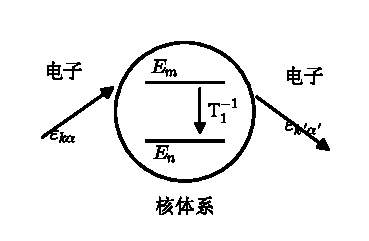
\includegraphics[width=6cm]{fig7-14.pdf}\\{\small 图 7.14\quad 核自旋系统与传导电子的散射过程}
\end{minipage}
\end{center}

其中包括了来自泡利不相容原理的概率因子 $f(\varepsilon)\left[1-f(\varepsilon')\right]$ 和保证散射过程总能量守恒的 $\delta$ 函数因子.由于在磁场中核自旋的能级差 $\left(E_{m}-E_{n}\right)$ 是一个可忽略的小量，它比 $k_{\mathrm{B}}T$ 和化学势 $\mu$ 均要小得多，可以认为散射前后电子态能量近似守恒，即可取近似 $\varepsilon_{k's'}\approx\varepsilon_{ks}\equiv\varepsilon$，这时式(7.7.12)中 $\delta$ 函数简化为 $\delta\left(\varepsilon_{ks}-\varepsilon_{k's'}\right)$.再进而考虑到，在实验温度范围内，总有 $k_{\mathrm{B}}T\ll\mu$，又可将概率因子演化为 $f(\varepsilon)\left[1-f(\varepsilon)\right]=\left(k_{\mathrm{B}}T\right)\left[-\mathrm{d}f(\varepsilon)/\mathrm{d}\varepsilon\right]\approx\left(k_{\mathrm{B}}T\right)\delta\left(\varepsilon-\mu\right)$.运用这两个 $\delta$ 函数，经求和化积分后，即可从式(7.7.12)求得 $T_{1}^{-1}(T)\propto T$ 的简单结果，此即柯林嘎关系 $T_{1}(T)\cdot T=$ 常数.

为使读者明白柯林嘎关系的成立是朗道费密液体行为的表现，可直接从金属的费密球模型（即费密液体模型）出发，对 $T_{1}^{-1}(T)$ 的特征作如下的定性解释：根据泡利原理，只有位于费密面附近 $\left(k_{\mathrm{B}}T\right)$ 范围内的传导电子才可以参与散射，即只占全部传导电子数的一个分数 $\left(k_{\mathrm{B}}T/\mu\right)$.引入费密面上态密度 $N(\mu)$，求得与核自旋发生散射的传导电子数为 $N(\mu)\left(k_{\mathrm{B}}T/\mu\right)$，它与接触势强度的模平方 $\left|V\right|^{2}$ 都应当是正比于核弛豫率的关键参数，由此立刻得到柯林嘎关系式：
\begin{equation}
  T_{1}^{-1}(T)\sim\left|V\right|^{2}\cdot N(\mu)\cdot\left(k_{\mathrm{B}}T/\mu\right)\propto T
  \qquad\text{或}\quad T_{1}(T)\cdot T=\text{常数}
\end{equation}
因此，柯林嘎关系的出现是与金属中存在费密面直接相关联的.在常规BCS超导体中，核自旋-点阵弛豫率的柯林嘎关系在 $T>T_{\mathrm{c}}$ 时普遍成立，表明其正常态具有费密液体行为.

在以 $\mathrm{YBa}_{2}\mathrm{Cu}_{3}\mathrm{O}_{7}$ 为代表的铜氧化合物高温超导体中，人们却观察到其正常态核自旋-点阵弛豫率的异常行为，特别是对于导电层中 $^{63}\mathrm{Cu}$ 的 $T_{1}^{-1}$ 测量，来自各著名研究组的数据基本上是一致的，均表明Y-123最佳化合物在 $T>T_{\mathrm{c}}$ 温区的核弛豫率满足经验公式
\begin{equation}
  T_{1}^{-1}(T)=aT+b
\end{equation}
其中a和b都是与温度无关的常数.在上式右边，随温度线性变化的 $aT$ 项与普通金属的柯林嘎行为定性一致，奇异之处在于出现了不随温度变化的常数b项，导致 $^{63}\mathrm{Cu}$ 的核弛豫明显偏离柯林嘎关系，呈现出不同于朗道费密液体的反常特征.使问题变得复杂的是，测量位于同一导电层中 $^{17}\mathrm{O}$ 的核弛豫，却表明其 $T_{1}^{-1}$ 是满足柯林嘎关系的，对于 $^{17}\mathrm{O}$ 没有异常项b出现.在Y-123最佳化合物中，位于同一个 $\mathrm{CuO}_{2}$ 平面上的 $\left(1/T_{1}\right)_{\mathrm{Cu}}$ 具有明显的非柯林嘎行为，而 $\left(1/T_{1}\right)_{\mathrm{O}}$ 则表现柯林嘎行为，二者有如此显著的定性差别，其理论解释自然应超出朗道费密液体范围.一个新的理论必须同时解释 $\left(1/T_{1}\right)_{\mathrm{Cu}}$ 的非费密液体特征和 $\left(1/T_{1}\right)_{\mathrm{O}}$ 的正常费密液体行为.

\subsection*{4. 反铁磁费密液体模型}

目前，在解释高温超导体核弛豫实验方面，比较成功的理论模型是密立斯（Millis）、莫尼恩（Monien）和派因斯（Pines）\textsuperscript{[33]}（MMP）提出的反铁磁费密液体（AFL）理论.他们假定在 $\mathrm{CuO}_{2}$ 平面内每个元胞只含一个 $S=1/2$ 的电子自旋自由度，其中心在Cu格点上，并且诸Cu格点的电子自旋之间存在着短程的反铁磁关联和相应的自旋涨落效应，这一关联使近邻Cu格点的电子自旋取向基本相反.密立斯等人认为正是Cu格点上的电子自旋与各类核磁矩的相互作用产生铜氧化合物中的核自旋-点阵弛豫.对于Cu的核弛豫，主要是考虑 Cu 核与同格点电子自旋的相互作用，可求出 $\left(1/T_{1}\right)_{\mathrm{Cu}}$ 的非柯林嘎关系，与经验公式(7.7.14)一致，其中不随温度变化的常数项b是反铁磁关联的自旋涨落效应产生的，从而解释了 $\left(1/T_{1}\right)_{\mathrm{Cu}}$ 的异常温度行为.对于O的核弛豫，则需要考虑O核与两个近邻Cu格点上的电子自旋互作用，因为在 $\mathrm{CuO}_{2}$ 平面中O位于两个近邻Cu格点之间，Cu与O的键长只是晶格常数的一半 $\left(a/2\approx0.2\ \mathrm{nm}\right)$，应有较强的互作用.但由于存在反铁磁关联，O的两近邻Cu格点的电子自旋取向相反，它们与O核磁矩的互作用将大部分相互抵消，导致在 $\left(1/T_{1}\right)_{\mathrm{O}}$ 中与温度无关的异常项消失，只剩下与温度成正比的柯林嘎项.这样MMP理论就同时解释了高温超导体中 Cu 与 O 的核弛豫的不同温度行为.

密立斯等人的反铁磁费密液体理论，只是在朗道费密液体理论基础上计入了反铁磁自旋涨落关联的修正.反铁磁费密液体理论，从本质上讲，仍属于费密液体范畴，我们仍可以沿袭前面的定性说法来理解核弛豫率异常的成因.当不计反铁磁关联时，反铁磁费密液体系统自然简化为朗道费密液体，这时费密面上的态密度基本上是与温度无关的常数，而参加散射的电子自旋激发仍然应限制在费密面附近 $k_{\mathrm{B}}T$ 范围内，于是得到弛豫率 $T_{1}^{-1}(T)\sim T$ 的柯林嘎关系，与式(7.7.13)相同.但是，当计入反铁磁自旋关联效应之后，由于关联随温度降低而增强，将对态密度产生重要的影响，使其中出现一个附加项 $\Delta N\left(\mu,T\right)\sim1/T$，表明低频自旋激发的态密度也将随温度降低而升高，正是此项与限制自旋激发范围的T因子相消，给出 Cu 核弛豫率的常数项b，导致 $\left(1/T_{1}\right)_{\mathrm{Cu}}$ 的非柯林嘎行为.在讨论O的核弛豫率时，由于来自两近邻Cu格点的反铁磁关联效应在O位上相互抵消，态密度仍与温度无关，这时 $\left(1/T_{1}\right)_{\mathrm{O}}$ 仍然满足柯林嘎关系，无异常行为.

密立斯等人的反铁磁费密液体理论不仅能正确解释Y-123与 La-214 等铜氧化合物中核自旋-点阵弛豫率的反常特性，还同时解释了核磁共振中的奈特（Knight）位移等磁响应实验.将该理论推广用于导电等电荷响应问题也获得了成功，例如在直流电阻率的讨论中，按照MMP模型应考虑载流子与位于Cu格点上的电子自旋自由度的耦合，文献\textsuperscript{[23]}中具体计算了载流子与反铁磁自旋涨落元激发（这种元激发在文献中称为反铁磁 paramagnons）散射的电阻率，所求得的零频 $\left(\omega=0\right)$ 散射率在 $T_{\mathrm{c}}$ 之上总能够满足 $\left(\hbar/\tau\right)\sim T$ 规律，合理说明了正常态的直流电阻率在相当宽阔的温区内是温度的线性函数.在这里是反铁磁自旋涨落（AFSF）机制产生电阻率反常，究其本源是电子系统内部的库仑关联作用所产生的.值得一提的是，载流子间通过交换反铁磁自旋涨落也可以产生有效吸引互作用，并且有利于形成 $d_{x^{2}-y^{2}}$ 波超导配对\textsuperscript{[23]}.到此为止，建立在反铁磁费密液体理论基础上的自旋涨落机制既能够说明正常态的电阻反常，又可以解释d波配对的形成，应当说对于最佳掺杂的高温超导体是一个有竞争力的理论.但是，最近在弱掺杂区发现的正常态能隙却对此理论提出了新的挑战，为此派因斯等人\textsuperscript{[34]}又提出了新的唯象假定，尚待实验证实.

\section{弱掺杂区正常态赝隙的发现}

根据§7中关于最佳掺杂样品的讨论，已使人们认识到高温超导体正常态的性质是十分反常的，需要用一个不同于朗道费密液体的理论描述.然而，当人们将注意力集中到相图中的弱掺杂区域时（见图7.5，其中最佳掺杂对应于最高的 $T_{\mathrm{c}}$ 点，其左边就是弱掺杂区，而右边称为过掺杂区），却观察到一个更令人吃惊的反常现象——在弱掺杂区的正常态（$T>T_{\mathrm{c}}$）中已经形成了能隙.换句话说，在通常情况下显示系统在 $T=T_{\mathrm{c}}$ 时进入超导态的能隙，现已在远远高于实际形成超导电性的温区内被观察到了.正常态能隙在文献中又称赝隙（pseudogap），所谓赝隙是指部分形成能隙，例如在单电子近似成立的能带论中，部分能隙说的是在费密面的部分区域中形成了能隙，而在其它区域中未成隙，系统仍保持金属性电导特征.尽管早期的观察仅在弱掺杂的YBCO（即弱掺杂的Y-123）样品中看到正常态有赝隙存在的迹象，但自从1996年当人们用ARPES直接测出赝隙存在之后，来自各不同实验组的测量结果均证实了一个共同的现象\textsuperscript{[31]}，即在所有弱掺杂的铜氧化合物高温超导体的正常态中均存在赝隙，这是弱掺杂区正常态的一个基本属性.

\subsection*{1. 弱掺杂区存在赝隙的间接证据}

1989年在测量弱掺杂 Y-123 导电层中铜（$^{63}\mathrm{Cu}$）的自旋-点阵弛豫率时，人们首次观察到赝隙存在的迹象.图7.15同时给出了 $T_{\mathrm{c}}=90$ K 的最佳掺杂样品 $\mathrm{YBa}_{2}\mathrm{Cu}_{3}\mathrm{O}_{7}$（□）和 $T_{\mathrm{c}}=60$ K 的弱掺杂样品 $\mathrm{YBa}_{2}\mathrm{Cu}_{3}\mathrm{O}_{6.7}$（○）中 $^{63}\mathrm{Cu}$ 的 $\left(T_{1}T\right)^{-1}$ 随温度的变化曲线.显然，在 $T_{\mathrm{c}}$ 以上最佳化合物正常态的 $\left(T_{1}T\right)^{-1}$ 随温度降低而增大并一直延伸到 $T_{\mathrm{c}}=90$ K 处，这是反铁磁自旋关联在降温时增强所产生的正常态非柯林嘎行为，可以用式(7.7.14)描述.当温度下降到 $T_{\mathrm{c}}$ 时，$\left(T_{1}T\right)^{-1}$ 曲线的明显转折和进入超导态后（$T<T_{\mathrm{c}}=90$ K 时）曲线的急剧下降则表明：在发生正常-超导相变的同时，载流子因配对形成了能隙，导致态密度的亏损，从而压制了Cu格点上电子自旋的激发，使 $\left(T_{1}T\right)^{-1}$ 曲线急剧下降.对于 $T_{\mathrm{c}}=60$ K 弱掺杂样品，在 $T>150$ K 的高温端的非柯林嘎行为与最佳化合物正常态的反常行为极其相似，这一反常仍来源于温度下降时AF自旋关联的增强效应，但是在 $150\ \mathrm{K}>T>100\ \mathrm{K}$ 的中间温区 $\left(T_{1}T\right)^{-1}$ 随温度缓慢变化并有一个极大值宽峰，表现出与 $T_{\mathrm{c}}=90$ K 最佳化合物明显的不同.然后当 $T<100$ K 时，尽管弱掺杂样品仍处于正常态，其 $\left(T_{1}T\right)^{-1}$ 已开始下降，而且是连续地下降和经过 $T_{\mathrm{c}}$（$T_{\mathrm{c}}=60$ K）进入超导态.在弱掺杂的 $T_{\mathrm{c}}=60$ K 样品中，$\left(T_{1}T\right)^{-1}$ 从正常态的某一温度 $T^{*}$（$T^{*}>T_{\mathrm{c}}$）所开始的连续下降与最佳化合物进入超导态后的下降趋势也是定性一致的.弱掺杂样品的这种不同寻常的中间温区自旋-点阵弛豫行为被认为是载流子在正常态的某一温度 $T^{*}$ 处已开始预配对并形成了能隙，这是显示正常态存在赝隙的第一个间接证据.

\begin{center}
\begin{minipage}{7cm}
\centering
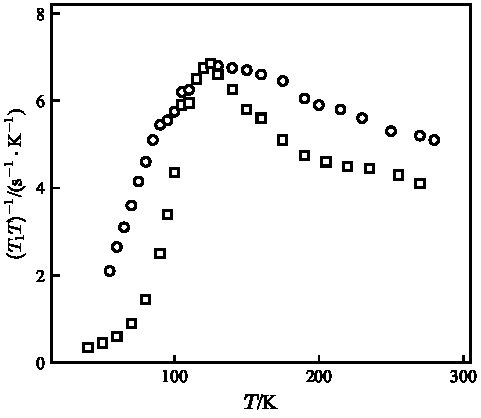
\includegraphics[width=7cm]{fig7-15.pdf}\\{\small 图 7.15\quad $\mathrm{YBa}_{2}\mathrm{Cu}_{3}\mathrm{O}_{6+x}$ 中 $^{63}\mathrm{Cu}$ 的核自旋-点阵弛豫率，其中最佳掺杂（□）为 $x=1$，}\\[0.2em]
{\small 弱掺杂（○）为 $x=0.7$}
\end{minipage}
\end{center}

另一个显示弱掺杂区存在赝隙的间接证据来自对导电层中直流电阻率 $\rho_{\mathrm{ab}}$ 的测量，图7.16是 $\mathrm{La}_{2-x}\mathrm{Sr}_{x}\mathrm{CuO}_{4}$ 在各种掺杂浓度x时的 $\rho_{\mathrm{ab}}$-$T$ 曲线，其中除最佳掺杂 $\left(x=0.15\right)$ 情形外，还包括了弱掺杂 $\left(x<0.15\right)$ 和过掺杂 $\left(x>0.15\right)$ 情形.在图7.16(a)中可以看出，除了 $x=0.15$ 曲线在 $T_{\mathrm{c}}$ 之上具有线性温度行为以外，其它的弱掺杂样品均在某一温度 $T^{*}(x)$ 之下明显偏离线性，并且 $T^{*}(x)$ 随x减小而升高，其中 $x<0.07$ 的那些曲线已不是超导样品，它们的基态为绝缘体.图7.16(b)主要显示过掺杂 La-214 系统 $\left(x>0.15\right)$ 的电阻率温度行为，这时随着x的逐渐增大 $T_{\mathrm{c}}$ 连续降低，最后在 $x=0.3$ 时变为非超导的正常金属，而其低温电阻率则演变为具有 $\rho_{\mathrm{ab}}\sim T^{2}$ 特征的朗道费密液体，与本章§2中所介绍的相图特征一致.

\begin{center}
\begin{minipage}{9cm}
\centering
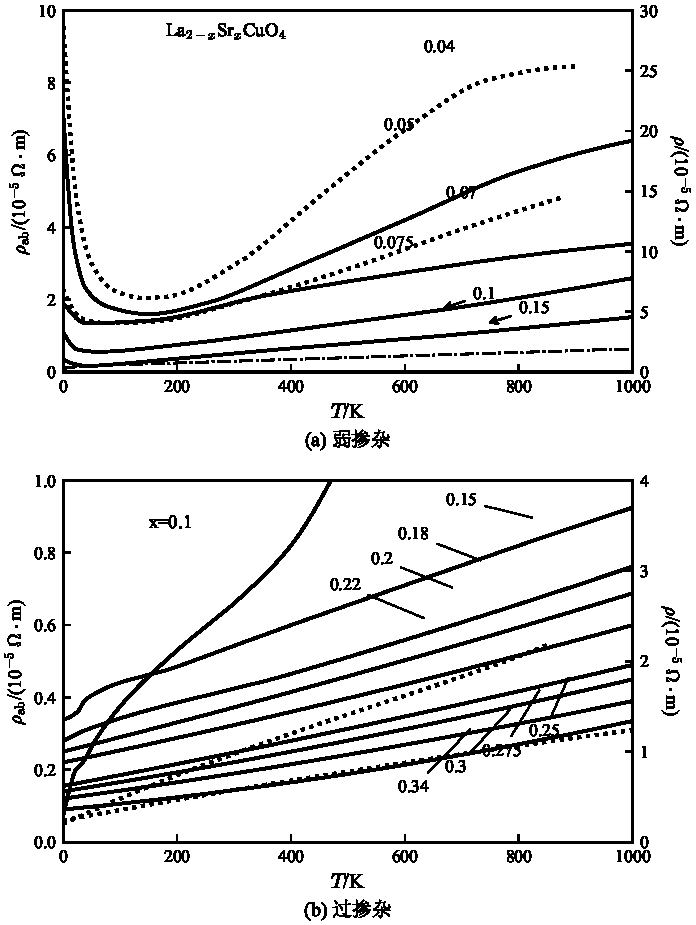
\includegraphics[width=9cm]{fig7-16.pdf}\\[0.3em]
{\small (a) 弱掺杂\qquad\qquad\qquad\qquad (b) 过掺杂}\\[0.2em]
{\small 图 7.16\quad $\mathrm{La}_{2-x}\mathrm{Sr}_{x}\mathrm{CuO}_{4}$ 在各种掺杂浓度 x 时的 $\rho_{\mathrm{ab}}$-$T$ 曲线}\\[0.2em]
{\small 其中点线为单晶（左标），实线代表多晶样品（右标）}
\end{minipage}
\end{center}

弱掺杂的 La-214 中电阻率偏离线性温度规律的特征在弱杂的Y-123化合物中也同样存在，考虑到正常态的线性电阻率可以用载流子被自旋涨落散射机制解释，在弱掺杂时电阻率在 $T<T^{*}$ 温区偏离线性温度律的更快降落也可以认为是由于在正常态形成了能隙，使自旋涨落效应受到压制的缘故，但是根据核弛豫率和电阻率实验来断言赝隙的存在都是间接的，带有一定的人为猜测性，还需要有赝隙存在的直接证据.

\subsection*{2. 弱掺杂区存在赝隙的直接证据}

角分辨光电子发射谱（简称ARPES）是直接测量准粒子态密度随能量和动量变化的有力工具.对于超导体运用APRES技术可以直接确定能隙的大小及其随取向 $\hat{\boldsymbol{k}}$ 的变化.因为当系统进入超导态后，能隙出现在准粒子的态密度中，这时 k 态的态密度将在低于费密能的某个能量［即能隙 $\Delta(\boldsymbol{k})$］范围内下降为零，相当于使态k态的态密度向低能方向移动而离开费密能，实验上表现为ARPES谱线前沿（leading edge）的中点有相应的移动.在§3中，人们正是测量ARPES谱的这一移动，定出了二维BZ中能隙 $\Delta(\boldsymbol{k})$ 随取向的变化，首次观察到铜氧化合物高温超导体的各向异性配对特征.因此，ARPES是直接测量能隙的一个重要手段.如果在欠掺杂铜氧化合物的正常态中确实存在能隙，其最为直接的证据应来自ARPES测量.1996年美国斯坦福大学研究组\textsuperscript{[35]}和阿贡研究组\textsuperscript{[36]}利用ARPES在 Bi-2212 欠掺杂样品中，都清楚地观测到在正常态中打开能隙的直接证据，并且这个正常态赝隙也具有 $d_{x^{2}-y^{2}}$ 波对称性（即沿 $k_{x}$ 与 $k_{y}$ 方向能隙取最大值，沿对角线 $\left|k_{x}\right|=\left|k_{y}\right|$ 方向则为能隙的零点），与§3中所介绍的最佳化合物在 $T_{\mathrm{c}}$ 以下的超导能隙具有相同的各向异性 $\left(d_{x^{2}-y^{2}}\right.$ 波）特征.他们的测量还表明：正常态能隙的起始温度随掺杂增加而减小，当系统成为最佳化合物时 $T^{*}$ 已十分接近 $T_{\mathrm{c}}$，这时在ARPES实验中已观察不到最佳掺杂以及过掺杂区的正常态能隙，可以认为在正常态出现赝隙只是弱掺杂区的特征.图7.17是考虑了弱掺杂区存在正常态赝隙的示意相图，正常态赝隙只出现在弱掺杂区，当系统进入最佳与过掺杂区时赝隙实际上已消失，只剩下 $T<T_{\mathrm{c}}$ 时的超导能隙.这时系统形成能隙与进入超导态几乎是同时发生的，而且在 $T=T_{\mathrm{c}}$ 时超导能隙消失，与常规BCS超导体的正常-超导转变特征相似.此外，在过掺杂区内BCS的普适关系 $\left[2\Delta(0)/k_{\mathrm{B}}T_{\mathrm{c}}\right]=$ 常数仍然成立.

\begin{center}
\begin{minipage}{7.5cm}
\centering
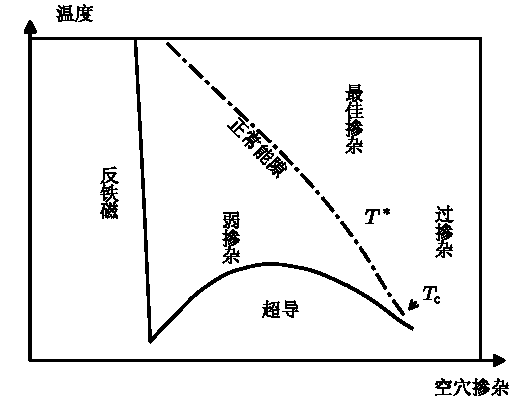
\includegraphics[width=7.5cm]{fig7-17.pdf}\\{\small 图 7.17\quad 计入赝隙的示意相图}
\end{minipage}
\end{center}

在弱掺杂样品中的ARPES测量直接证实了正常态能隙的存在当然是一个重要的新发现，但却是不出人们所料的结果.令人感到十分惊奇的是，还发现了下列完全不同于BCS超导相变的特征：其一是正常态赝隙（PG）仅在超过起始温度 $T^{*}$ 时（对于弱掺杂的 Bi-2212，$T^{*}$ 在170～300 K之间）才迅速下降为零，在 $T<T^{*}$ 的大部分正常区域中PG几乎不随温度变化，而且正常态PG的数值与 $T\ll T_{\mathrm{c}}$ 时的超导能隙值相近.包括ARPES在内的多种实验均已证实\textsuperscript{[31]}，随着温度降低正常态的PG平坦连续地演变为超导能隙，特别当温度经过 $T_{\mathrm{c}}$ 时能隙的数值并无显著的变化.换句话说，没有任何实验证据表明弱掺杂区中超导能隙在 $T=T_{\mathrm{c}}$ 处降为零，从根本上不同于BCS超导体的序参数特征.在BCS超导体中，表征序参数的超导能隙在 $T_{\mathrm{c}}$ 处应消失，即有 $\Delta_{\mathrm{BCS}}\left(T_{\mathrm{c}}\right)=0$ 关系.其二是ARPES的测量还表明：在弱掺杂区域中在掺杂增加（即 $T_{\mathrm{c}}$ 升高）的同时，正常态的PG与零温的超导能隙均不按比例增大，反而呈现微弱的下降趋势，这种异常的变化趋势完全与BCS理论的预言相反，在BCS超导体中，零温超导能隙值应与 $T_{\mathrm{c}}$ 值成正比，并存在 $\left[2\Delta_{\mathrm{BCS}}(0)/k_{\mathrm{B}}T_{\mathrm{c}}\right]=$ 常数的普适关系，但是对于弱掺杂的铜氧化合物高温超导体，这一BCS的普适关系已不成立.正如安德逊所指出：“在这里的情形已不再是BCS理论所能解释的，尽管仍然存在库柏对，但其相变的物理内涵已与常规超导体的行为相去甚远，已经不能再称为BCS超导相变了.”\textsuperscript{[37]}

\subsection*{3. 小结与讨论}

尽管以上所介绍的赝隙测量主要是在含有两个 $\mathrm{CuO}_{2}$ 层的 Y-123 及 Bi-2212 欠掺杂化合物中作出的，但随后的实验表明，无论是在含单 $\mathrm{CuO}_{2}$ 层的 Hg-1201 及 La-214 中，或者是在含有三个 $\mathrm{CuO}_{2}$ 层的 Hg-1223 等弱掺杂化合物中都观察到与双层弱掺杂化合物中相似的赝隙特征.我们可以说，存在正常态赝隙是所有铜氧化合物高温超导体在弱掺杂区的普遍特征.无论是关于自旋响应，还是关于电荷响应的测量均已证实存在一个特征温度 $T^{*}$，它远比 $T_{\mathrm{c}}$ 高得多，在这个温度处出现正常态的配对，形成赝隙.赝隙存在于正常态的 $T^{*}<T<T_{\mathrm{c}}$ 温区之内.在弱掺杂区，当掺杂浓度增加时，$T_{\mathrm{c}}$ 升高，赝隙的起始温度 $T^{*}$ 则随之下降，在最佳掺杂时两者已十分接近，一旦进入过掺杂区，$T^{*}$ 即并入 $T_{\mathrm{c}}$ 曲线，这时已观察不到正常态的赝隙.因此，图7.17中的 $T^{*}$ 与 $T_{\mathrm{c}}$ 曲线构成了赝隙区的边界，它主要出现在弱掺杂区.实验还证实正常态赝隙与超导能隙具有相同的d波对称性，而且没有任何证据说明超导能隙在转变温度 $T_{\mathrm{c}}$ 处可能降为零.因此在铜氧化合物高温超导体的弱掺杂区域中，在正常态的 $T^{*}$ 温度以下已经形成了配对，并显示出赝隙的存在，但还没有发展成为一个长程相干的库柏对系统，只有在更低的温度 $T_{\mathrm{c}}$ 之下才能形成库柏对间的相位相干，并发生超导凝聚.在这里对的形成与超导凝聚不是同时发生的，它们将分成两步在不同的温度上发生.这是与BCS完全不同的图像，在BCS理论中，对的形成与相位相干是同时发生的.但是，在欠掺杂的铜氧化合物中，实验已证明当尚未发生超导凝聚时，在正常态已有能隙打开，这表明在正常态首先形成了电子间的“预配对”，而后才发生相干凝聚进入超导态.更确切地说，在正常态的“预配对”观点是人们根据弱掺杂区普遍存在赝隙现象所达成的共识.

最早提出的“预配对”模型是安德逊的共振价键（resonating valence bond 以下简称RVB）模型\textsuperscript{[38]}.首先说明，所谓价键态是指两个自旋间配对所形成的单重态，在价键（VB）态基础上将所有可能的自旋单重态配对波函数按照量子力学的叠加原理作线性组合就构成共振价键态.安德逊认为在掺杂的铜氧化合物中RVB态比反铁磁奈耳（Neel）态更稳定和更接近系统的基态，因此他建议从RVB态出发讨论高温超导电性.在未掺杂的RVB态中，每个格点上有一个电子，这个电子的自旋自由度与另一格点上电子的自旋配对，组成总自旋为零的自旋单态，而RVB的基态波函数就是点阵中的不同格点间的自旋单重配对态的线性组合，这时系统中的每一个自旋都被冻结在单重配对态之中，从而构成RVB理论中电中性的“真空”.现在若从此“真空”中某格点上取出一个电子（即进行空穴掺杂），则相对于RVB“真空”讲，在此格点上将出现一个无自旋但带有 $\left(+e\right)$ 电荷的准粒子（即空穴子），与此同时还有另一个格点上的自旋由于失配而不能形成自旋单态，相对于RVB“真空”在失配的格点上将出现一个带有 $S=1/2$ 自旋但无电荷的准粒子（即自旋子）.安德逊认为空穴子（holons）与自旋子（spinons）是RVB背景上的两种相对独立运动的准粒子，它们分别反映电荷自由度与自旋自由度的运动特征，此即文献中经常提到的电荷与自旋分离假说.在这个意义上人们常说RVB图像是一个基于自旋与电荷分离假定的模型.由于在RVB图像中自旋自由度的单重态配对已经在远高于 $T_{\mathrm{c}}$ 时形成，必然导致在自旋激发谱中出现正常态的能隙，对应于实验上观察到的赝隙或自旋能隙（spin gap），而超导电性的出现还取决于空穴子之间的相干性，仅当空穴子在 $T_{\mathrm{c}}$ 时成为相位相干时，系统才能凝聚为超导态.在强关联电子系统中，常采用费密子描述有自旋但无电荷的自旋子，而将带有电荷却无自旋的空穴子当作带电玻色子，因此人们认为在RVB态上的超导就是荷电玻色子的玻色凝聚.但应明白，这是在已经形成自旋单重态配对基础上的空穴子凝聚.在第十一章中我们将介绍基于RVB态的一个高温超导平均场理论（§10），用于定量解释在弱掺杂区形成赝隙（即预配对）与超导凝聚（即玻色凝聚）发生在不同的温度.目前RVB理论已超出平均场近似，其中受到人们普遍关注的是李雅达等人提出的规范场理论\textsuperscript{[39]}.RVB理论中最基本的假定是认为在二维强关联电子体系中存在电荷与自旋分离的两种元激发.但是这个基本假定还有待于实验的证实，而理论上则涉及二维拉亭格液体的研究\textsuperscript{[40]}.人们寄希望于二维拉亭格理论能够支持 $\mathrm{CuO}_{2}$ 平面上的自旋与电荷分离假定.

\begin{canKao}
\begin{enumerate}[label={[\arabic*]}, leftmargin=2.2em, itemsep=0pt]
\item 章立源等. 超导物理. 北京: 电子工业出版社，1987
\item Bednorz J D, Müller K A. Z Phys, 1986, B64: 189
\item Wu M K, Chu C W et al. Phys Rev Lett, 1987, 58: 908
\item 赵忠贤等. 科学通报，1987，32：412
\item Chu C W et al. Phys Rev Lett, 1988, 60: 941
\item Sheng Z Z et al. Phys Rev Lett, 1988, 60: 937
\item Tokura Y et al. Nature, 1989, 337: 345
\item Ginsberg D M. Physical Properties of High Temperature Superconductors (Vol IV). Singapore: World Scientific, 1994. 3
\item Levi B G. Phys Today, 1994, 47: 17
\item Gunnarsson O. Nature, 2000, 408: 528
\item Schön J H, Kloc Ch, Batlogg B. Nature, 2000, 408: 549; Science, 2001, 23: 2432
\item Bud'ko S L et al. Phys Rev Lett, 2001, 86: 1877
\item 韩汝珊. 高温超导物理. 北京: 北京大学出版社，1998
\item Zhang S C. Science, 1997, 275: 1089
\item Batlogg B. Phys Today, 1991, 44: 44
\item Shen Z X et al. Phys Rev Lett, 1993, 70: 1553
\item Wollman D A, van Harlingen D J et al. Phys Rev Lett, 1993, 71: 2134; 1995, 74: 797
\item Mathai A, Wellstood F C et al. Phys Rev Lett, 1995, 74: 4523
\item Tsuei C C, Kirtley F C et al. Phys Rev Lett, 1995, 73: 593
\item Kouznetsov K A et al. Phys Rev Lett, 1997, 79: 3050
\item Meservey R, Schwartz B B. Superconductivity (Vol 1). New York: Marcel Dekker Inc, 1969. 126
\item Frank J P et al. Ginsberg D M, ed. Physical Properties of High Temperature Superconductivity (Vol IV). Singapore: World Scientific, 1994. 189
\item Scalapino D J. Physics Reports, 1995, 250: 329
\item Tsuei C C et al. Phys Rev Lett, 1990, 65: 2724
\item Anderson P W, Morel P. Phys Rev, 1961, 123: 1911
\item Varma C M. Comments Solid State Phys, 1985, 11: 221
\item Stewart G R. Rev Mod Phys, 1984, 56: 755
\item Grewe N, Steglich F. Handbook on the Physics and Chemistry of Rare Earths, 1991, 14: 343
\item 邢定钰. 张其瑞主编. 高温超导电性. 杭州: 浙江大学出版社，1992. 第四章
\item Ziman J M. Electrons and Phonons. London: Oxford Univ Press, 1960. 364
\item Timusk T et al. Rep Prog Phys, 1999, 62: 61
\item Burns G. Solid State Physics. Orlando: Academic Press, 1985
\item Millis A J, Monien H, Pines D. Phys Rev, 1990, B44: 167
\item Pines D. Z Phys, 1997, B103: 129
\item Loeser A G et al. Science, 1996, 273: 325
\item Ding H et al. Nature, 1996, 382: 51
\item Levi B G. Phys Today, 1996, 49: 17
\item Anderson P W. Science, 1987, 235: 1196
\item Lee P A et al. Phys Rev Lett, 1997, 78: 4111
\item Anderson P W. Phys Rev Lett, 1991, 67: 2092
\end{enumerate}
\end{canKao}
